\documentclass[a4paper]{article}
\usepackage{fontspec}
\usepackage[russian]{babel}
\usepackage{amsmath}
\usepackage{amssymb}

\usepackage[a4paper]{geometry}
\usepackage{indentfirst}
\usepackage{color}
\usepackage{graphicx}
\usepackage{caption}
\usepackage{subcaption}

\setmainfont{CMU Serif}
\setsansfont{CMU Sans Serif}

\usepackage[backend=biber]{biblatex}
\addbibresource{refs.bib}

\newcommand{\tbd}[1]{
    \textcolor{red}{#1}
}
\newcommand{\tworowcell}[2]{
    \begin{tabular}{@{}c@{}}#1 \\ #2\end{tabular}
}
\renewcommand{\setminus}{\mathbin{\backslash}}

\begin{document}

\title{Рассмотрение методов отбора признаков и эталонов на примере задачи распознавания телевизионной рекламы в видеопотоке}
\author{Антон Ларин\\ М0813-2 \and Сергей Ларин\\ М0816-2 \and Владислав Соврасов\\ М0813-2}
\date{\today}
\maketitle

\begin{abstract}
В данной работе производится обзор методов отбора признаков (feature selection) и отбора эталонов (instance selection), служащих для сокращения размера задачи машинного обучения. Приводятся описания методов PCA, отбора признаков на основе случайного леса и методов CNN, FCNN, CCIS отбора эталонов. Также обсуждаются результаты их применения к модельной задаче распознавания телевизионной рекламы в видеопотоке.
\end{abstract}

\section{Введение}
Задача распознавания рекламы в видео с развитием вычислительных средств становится всё более доступной. Она является актуальной как для компаний, занимающихся кабельным вещанием или его мониторингом, так и для простых пользователей, желающих записывать и хранить передачи без рекламы.
Одним из имеющихся на рынке средств, позволяющих решать задачу, является редактор Nero Vision, входящий в состав известного пакета Nero Suite. Неизвестно, какой алгоритм при этом используется, но для его работы достаточно обычного домашнего компьютера.
\par
С точки зрения машинного обучения эта задача является задачей бинарной классификации: необходимо пометить каждый кадр видеопотока как содержащий рекламу или нет. В данной работе будет рассмотрена модельная задача распознавания. На её примере планируется рассмотреть работу некоторых методов машинного обучения и техник сокращения объёма данных, требуемых для обучения.
\section{Описание задачи и методологии работы}


\section{Отбор признаков}

\begin{Отбор признаков}
Основныя цели отбора признаков - уменьшение размерности задачи, а также выявление и отбрасывание признаков,
 не несущих полезной для решения задачи информации. Снижение размерности также ведёт к уменьшению времени обучения алгоритмов и уменьшению размера, занимаемого тренировочной выборкой.
 \par
Для рассматриваемого набора данных большая часть переменных не меняет значений на всех объектах выборки,
 поэтому все признаки с нулевой дисперсией были отброшены. В результате размерность задачи была сокращена
 с 4125 до около 230 переменных (227-229 в зависимости от канала). Такая ситуация произошла из-за использования схемы Bag of Words при создании датасета. 
 \subsection{PCA}
 \begin{PCA}
 Для дальнейшего уменьшения количества признаков использовался метод главных компонент
 (principal component analysis или PCA). Этот метод позволяет снизить размерность оптимальным с точки зрения некоторого критерия образом. Рассмотрим его подробнее.
 \par
 Постановка задачи, решаемой в методе PCA звучит следующим образом: найти линейное многообразие заданной 
 размерности, сумма квадратов расстояний до которого от данной системы точек минимальна. Стоит обратить внимание на то, что информация о принадлежности точек к какому-либо классу здесь не учитывается.
 Пусть \( X_i \subseteq \mathbb{R}^n, i=\overline{1,m} \) - набор произвольных векторов. Требуется найти векторы \(v_0\ldots v_d\subseteq \mathbb{R}^d, \Vert v_j \Vert = 1, v_i \bot v_j, j \neq  i, d \leq n\), задающие линейное многообразие L так, чтобы \(
 \sum_{i=1}^{m} dist^2(X_i, L) = \sum_{i=1}^{m}\Vert X_i - v_0 - \sum_{j=1}^k\langle X_i - v_0; v_j\rangle\ v_j \Vert\rightarrow min\)
 \subsection*{Результаты применения PCA}
 \begin{Результаты применения PCA}
 Лучшие результаты при уменьшении размерности с помошью PCA показал алгоритм random forest.
 \begin{figure} \centering 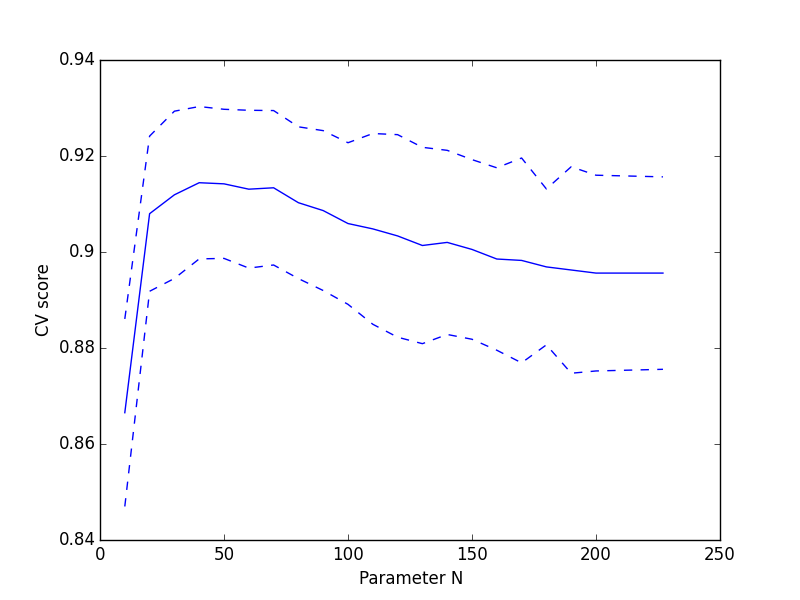
\includegraphics{images/randforest_NDTV_PCA.png} \caption{Random forest on NDTV } \label{fig:image} \end{figure}
 При одновременном улучшении результата кроссвалидации практически линейно уменьшается время обучения алгоритма.
  \begin{figure} \centering 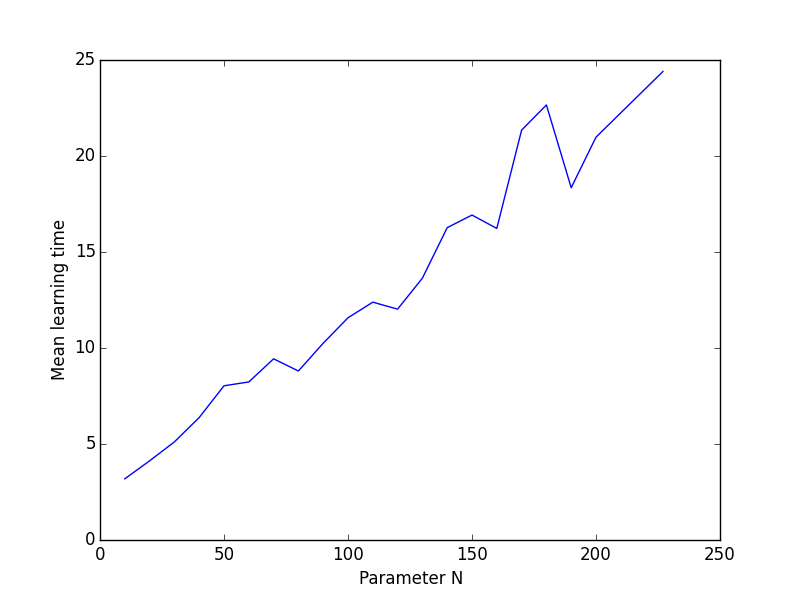
\includegraphics{images/randforest_NDTV_PCA_time.png} \caption{Random forest on NDTV train time} \label{fig:image} \end{figure}

\section{Отбор объектов обучающей выборки}
Как правило, работа с выборками большого объёма сопряжена с большими затратами временина обучение модели. Кроме этого, в достаточно популярном методе \(k\) ближайших соседей обучающая выборка хранится полностью, что в случае выборки большого объёма является ограничиващим для него фактором. Таким образом, привлекательными кажутся техники, которые позволяют уменьшить объём обучающей выборки, почти не теряя обобщающей способности. Данная тематика в литературе на английском языке называется instance selection (prototype selection).

В \cite{ps-taxonomy} было проведено крупномасштабное исследование, а также классификация методов отбора объектов обучающей выборки. Авторы также классифицировали их на следующие группы по механизму работы:
\begin{itemize}
    \item методы сгущения (condensation) --- стремятся сократить число точек, далёких от границ классов, в предположении, что они слабо влияют на геометрию границы. Они стремятся сохранить качество классификации на обучающей выборке, при этом качество классификации на тестовой выборке может пострадать. Тем не менее, они, как правило, достигают высокой степени сокращения объёма обучающей выборки;
    \item методы редактирования (edition) --- стремятся сократить число точек, близких к границам классов, несогласованных с соседними, шумовых точек. Данные методы создают более гладкие границы между классами, и приводят к повышению обобщающей способности классификатора, но они в меньшей степени сокращают объём выборки, чем методы предыдущей группы;
    \item гибридные методы (hybrid) --- стремятся найти подмножество выборки как можно меньшей мощности, которое улучшает обобщающую способность на тестовых данных.
\end{itemize}

Столкнувшись со значительными затратами вычислительных ресурсов при тестировании различных методов машинного обучения в нашей задаче, мы решили опробовать несколько методов отбора объектов и оценить, насколько большую пользу они могут принести в данной задаче. В пакете scikit-learn данный класс методов не представлен, а существующие реализации на Python \cite{scikit-protopy} показали себя неудовлетворительно с точки зрения производительности. Поэтому для проведения данной работы некоторые методы, реализованные авторами \cite{ps-taxonomy}, были портированы на язык C. В следующих подразделах выбранные методы отбора объектов описаны и приведены результаты, показанные ими на нашей задаче.

\subsection{Condensed nearest neighbor}
Данный метод хронологически является одним из первых методов отбора эталонов. Он был описан в 1966 году в \cite{hart} вместе с понятием согласованного подмножества (consistent subset) обучающей выборки \(T\) --- такого подмножества \(S\subseteq T\), что метод ближайшего соседа, обученный на \(S\) правильно классифицирует \(T\setminus S\). Он представляет из себя простейший метод сгущения и оперирует с двумя множествами: \(S\) и \(R\). Изначально \(S\) содержит лишь первый элемент обучающей выборки, а \(R=\varnothing\). Второй элемент классифицируется методом ближайшего соседа на основе множества \(S\), и, если ему присвоен верный класс, то он добавляется в \(R\), иначе он добавляется в \(S\). Каждый следующий элемент \(T\) обрабатывается аналогичным образом. После первого прохода через \(T\) процедура начинает совершать проходы через множество \(R\), до тех пор, пока за весь проход через \(R\) ни один элемент не будёт перенесён в \(S\), после чего в \(S\) находится согласованное подмножество \(T\).

Метод CNN был сформулирован для метода одного ближайшего соседа, однако расширение на \(k\) ближайших соседей производится очевидным образом: при классификации очередного элемента \(T\) (а впоследствии \(R\)) используется метод \(k\)NN с обучающей выборкой \(S\). Стоит отметить, что данный метод строит согласованное подмножество только по отношению к методу \(k\) ближайших соседей (для конкретного \(k\)), результирующее подмножество \(S\) не обязано быть согласованным для произвольного алгоритма классификации.

Были проведены эксперименты с методом CNN для \(k\in\{1, 5, 10\}\). На рис.~\ref{fig:cnn-stats} указаны результаты, показанные непосредственно CNN: время работы и доля отобранных объектов. 

\begin{figure}[h!]
    \centering
	\begin{subfigure}{0.45\textwidth}
		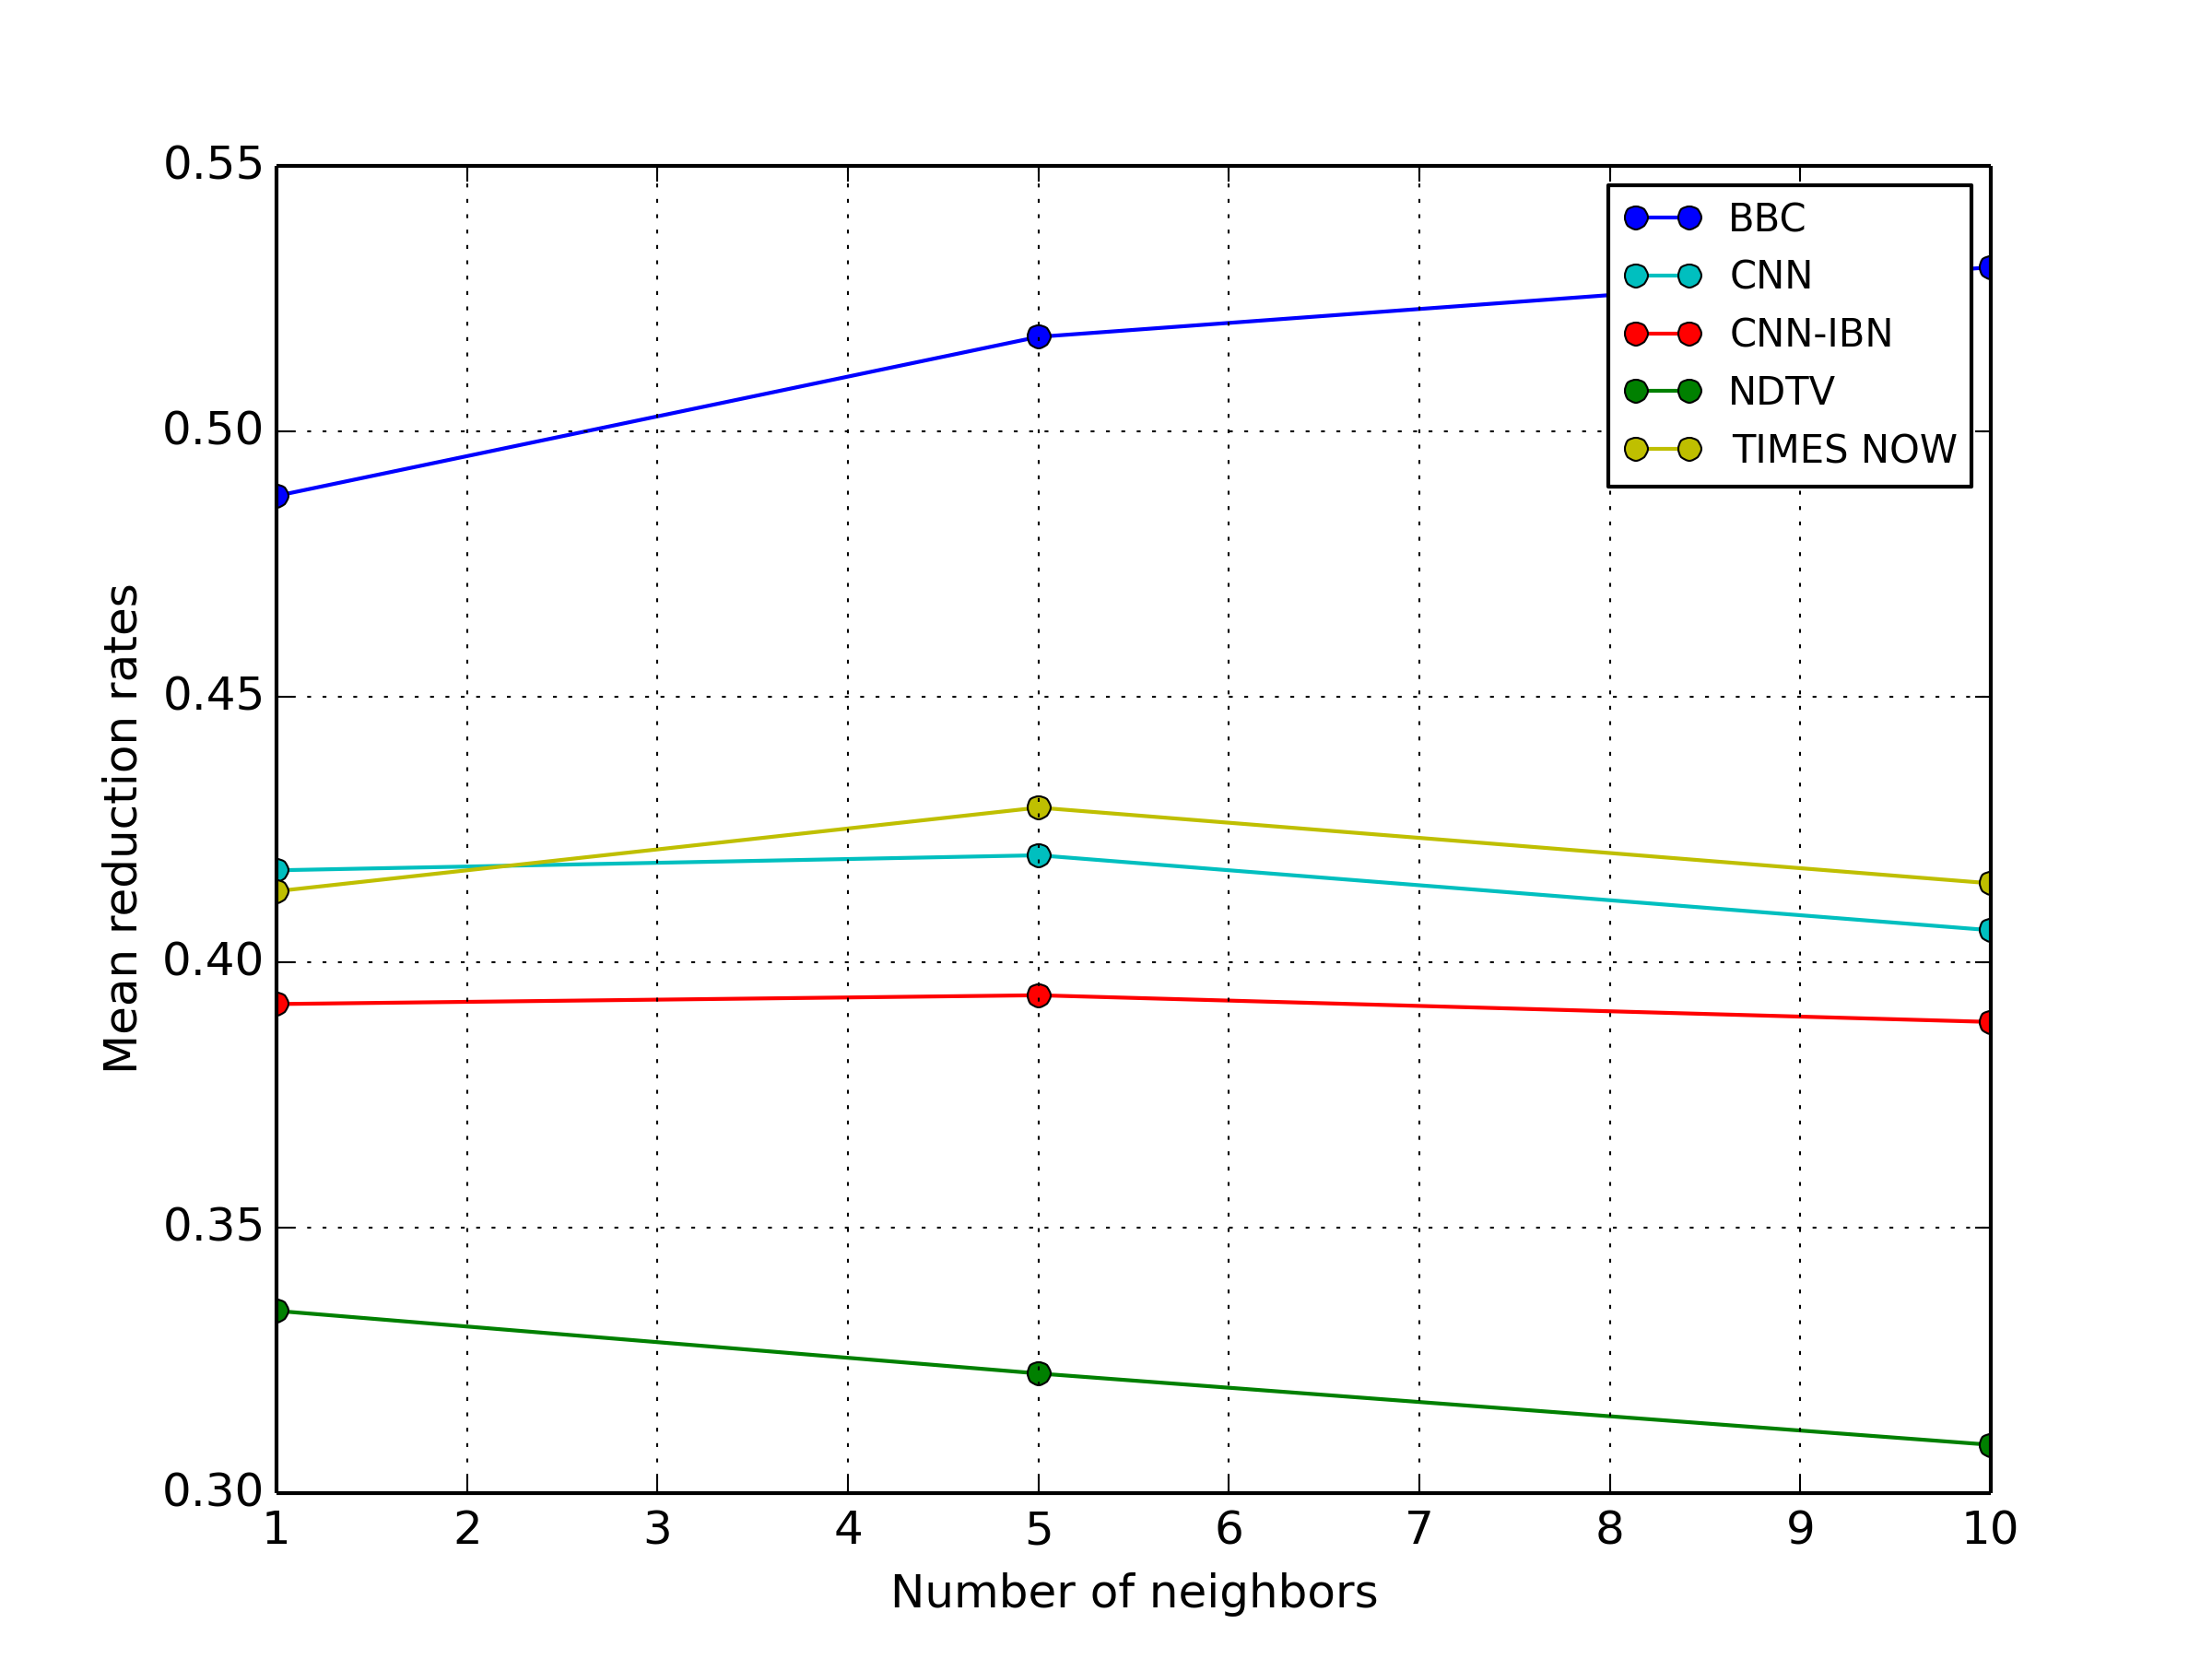
\includegraphics[width=\textwidth]{images/cnn-stats.png}
		\caption{Доля отобранных объектов.}
	\end{subfigure}
	\begin{subfigure}{0.45\textwidth}
		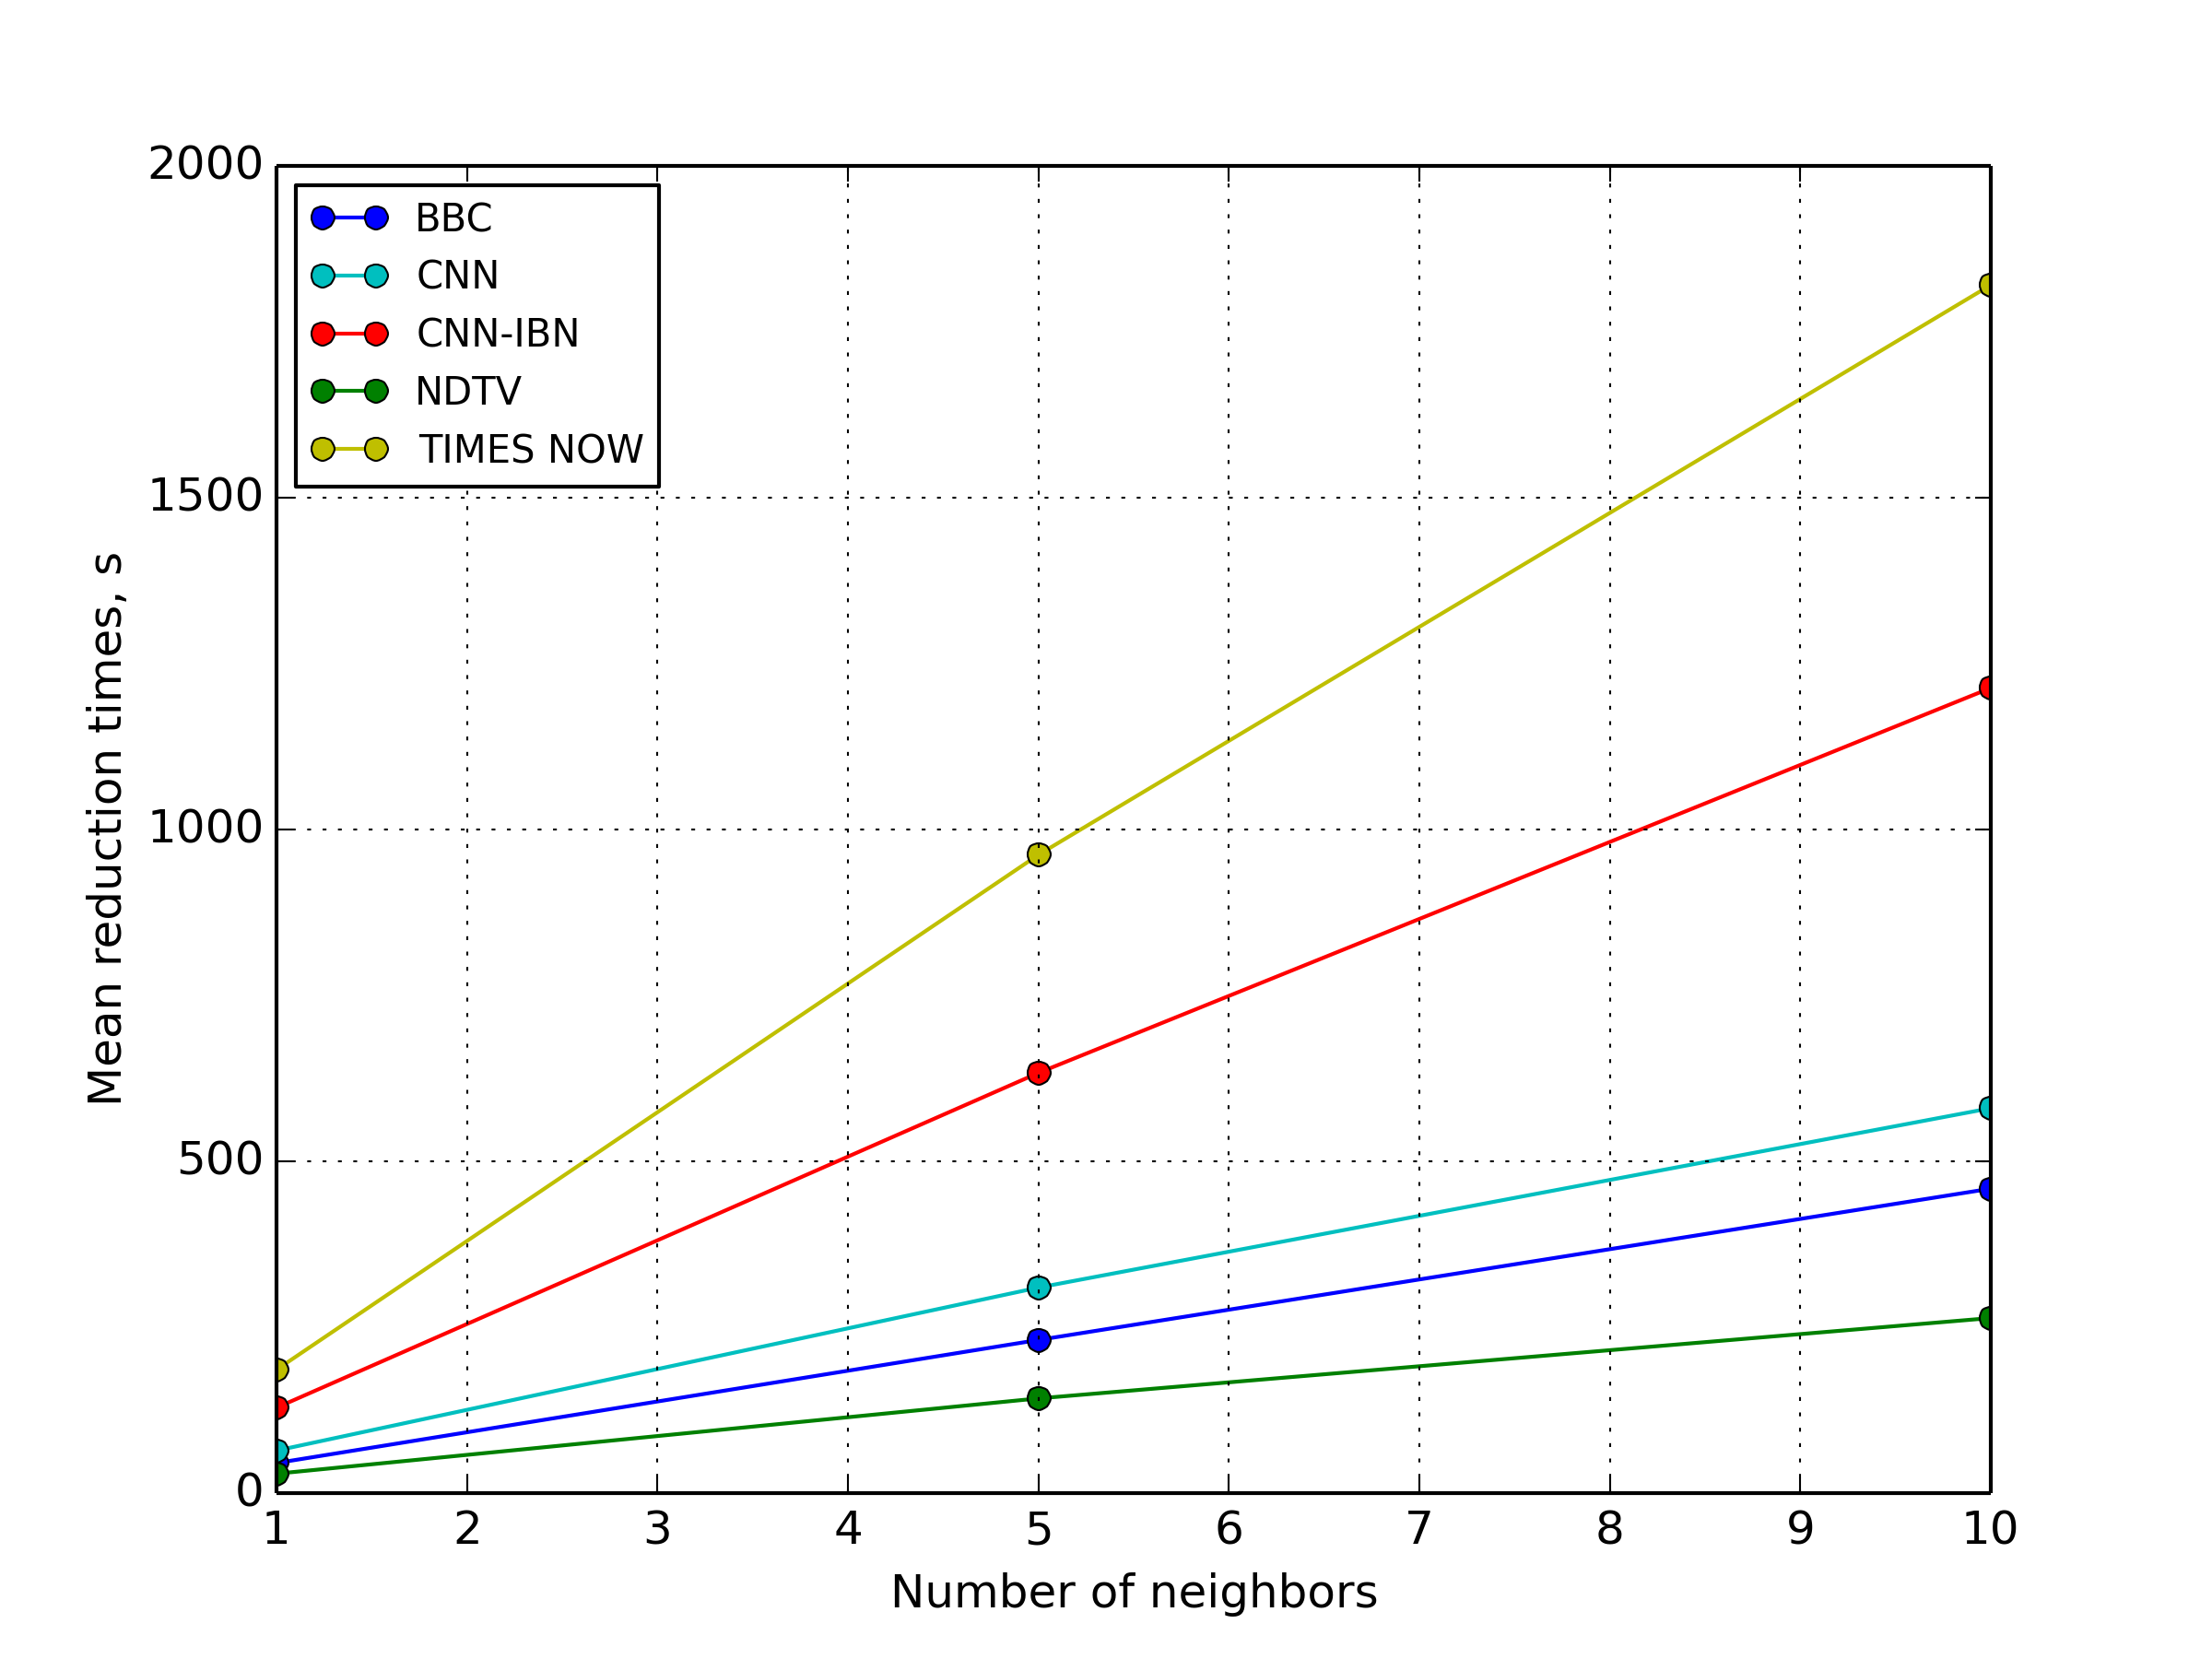
\includegraphics[width=\textwidth]{images/cnn-TimeStats.png}
		\caption{Время, потраченное на отбор эталонов.}
	\end{subfigure}
	\caption{Результаты работы CNN.}\label{fig:cnn-stats}
\end{figure}

На рис.~\ref{fig:cnn-knn-results}--\ref{fig:cnn-gtb-results} приведены результаты работы базовых методах на обучающих выборках, редуцированных с помощью CNN. \tbd{analysis}

\begin{figure}[h!]
    \centering
	\begin{subfigure}{0.45\textwidth}
		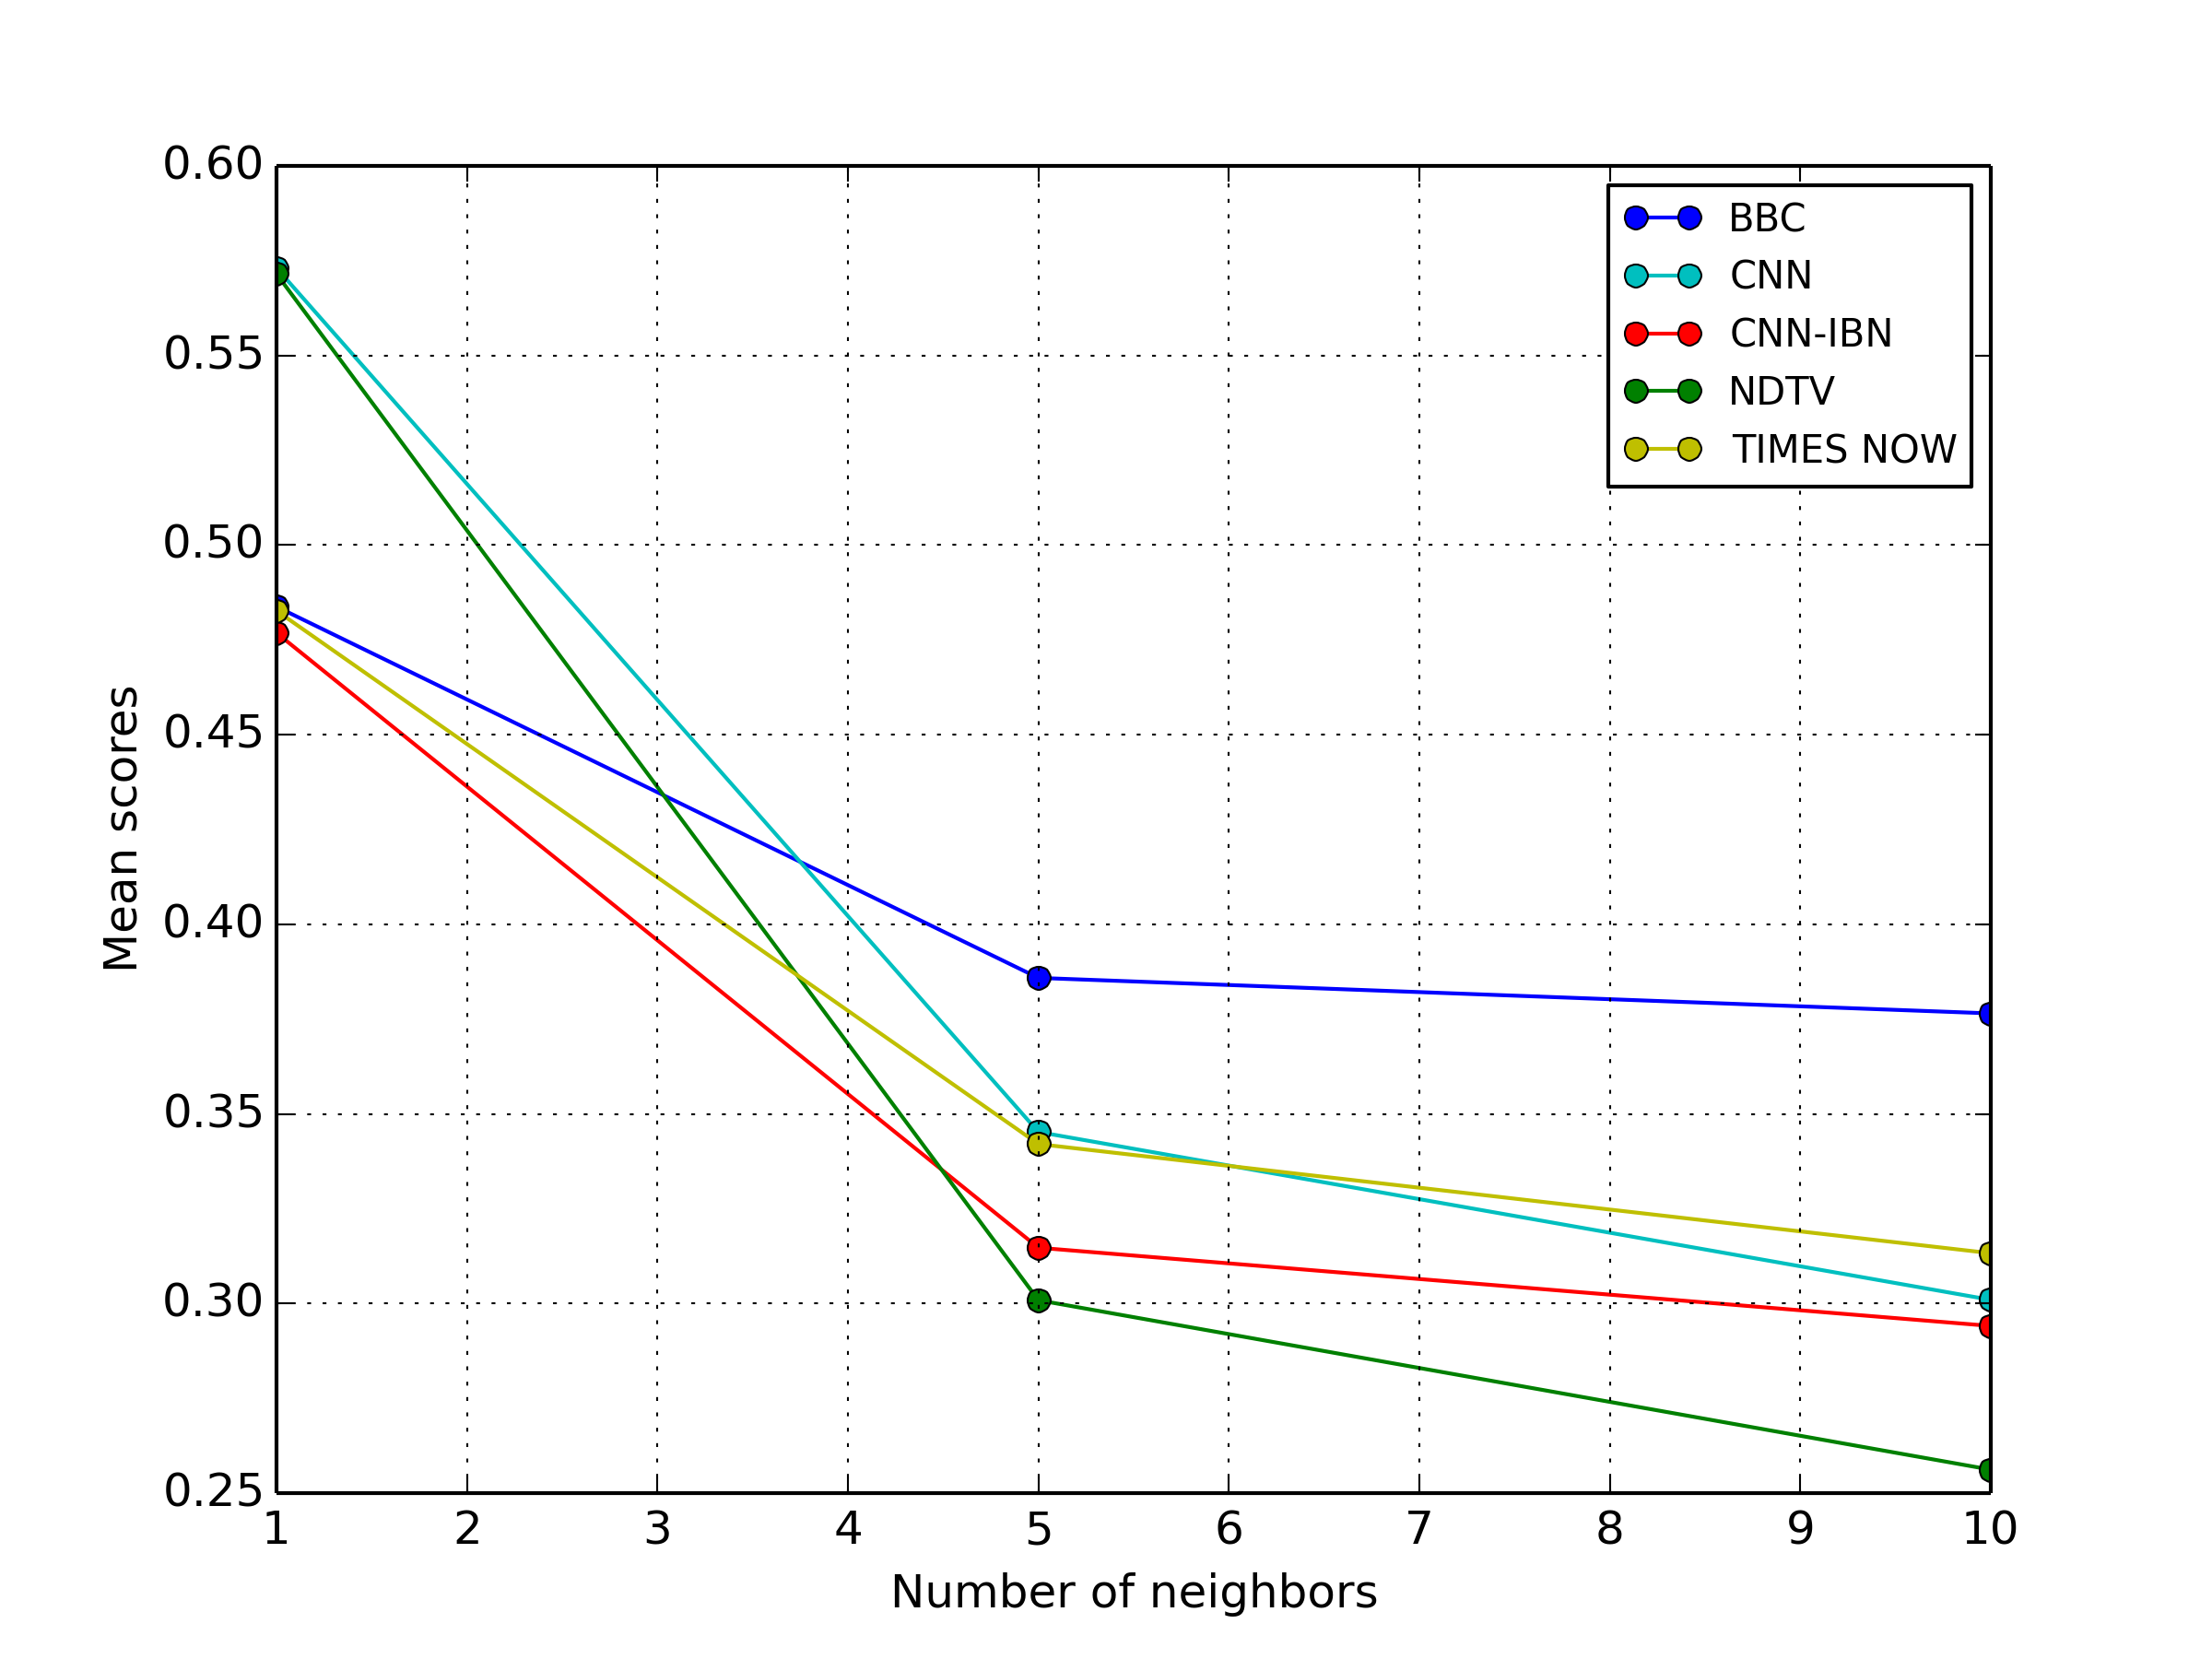
\includegraphics[width=\textwidth]{images/cnn-KNN.png}
		\caption{Качество классификации.}
	\end{subfigure}
	\begin{subfigure}{0.45\textwidth}
		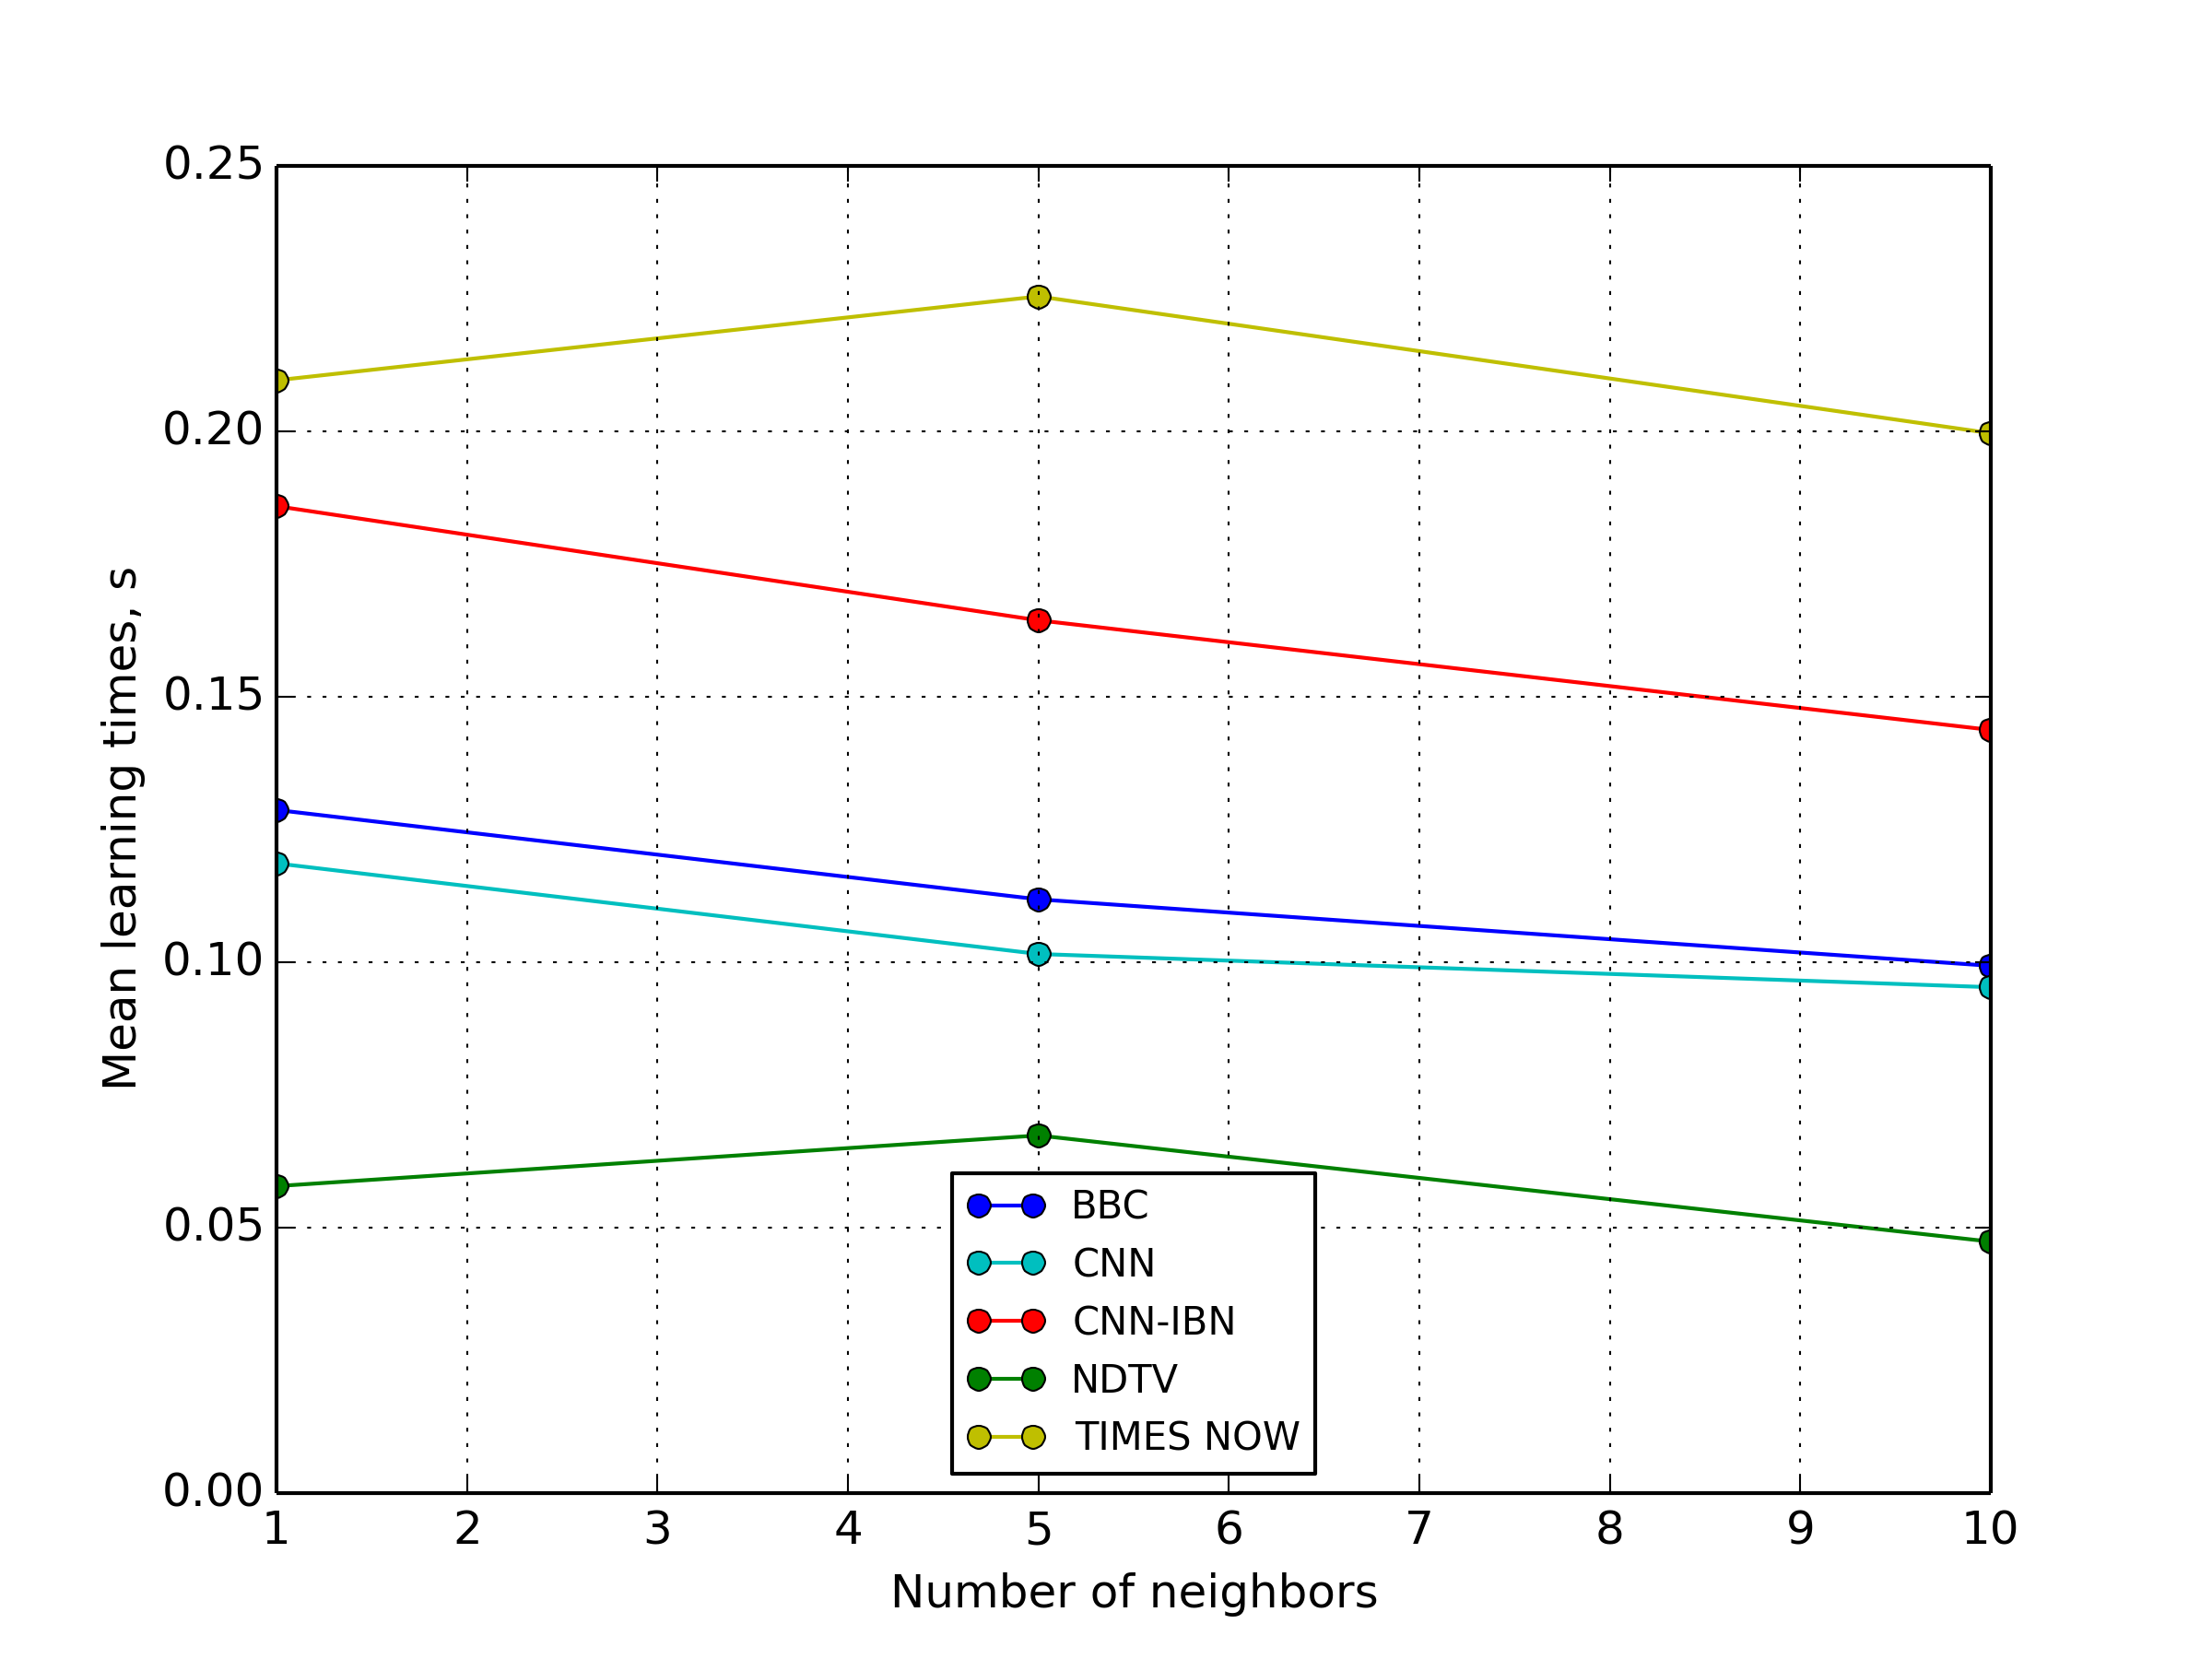
\includegraphics[width=\textwidth]{images/cnn-KNNTime.png}
		\caption{Время обучения.}
	\end{subfigure}
	\caption{Результаты применения CNN для 15-NN.}\label{fig:cnn-knn-results}
\end{figure}

\begin{figure}[h!]
	\centering
	\begin{subfigure}{0.45\textwidth}
		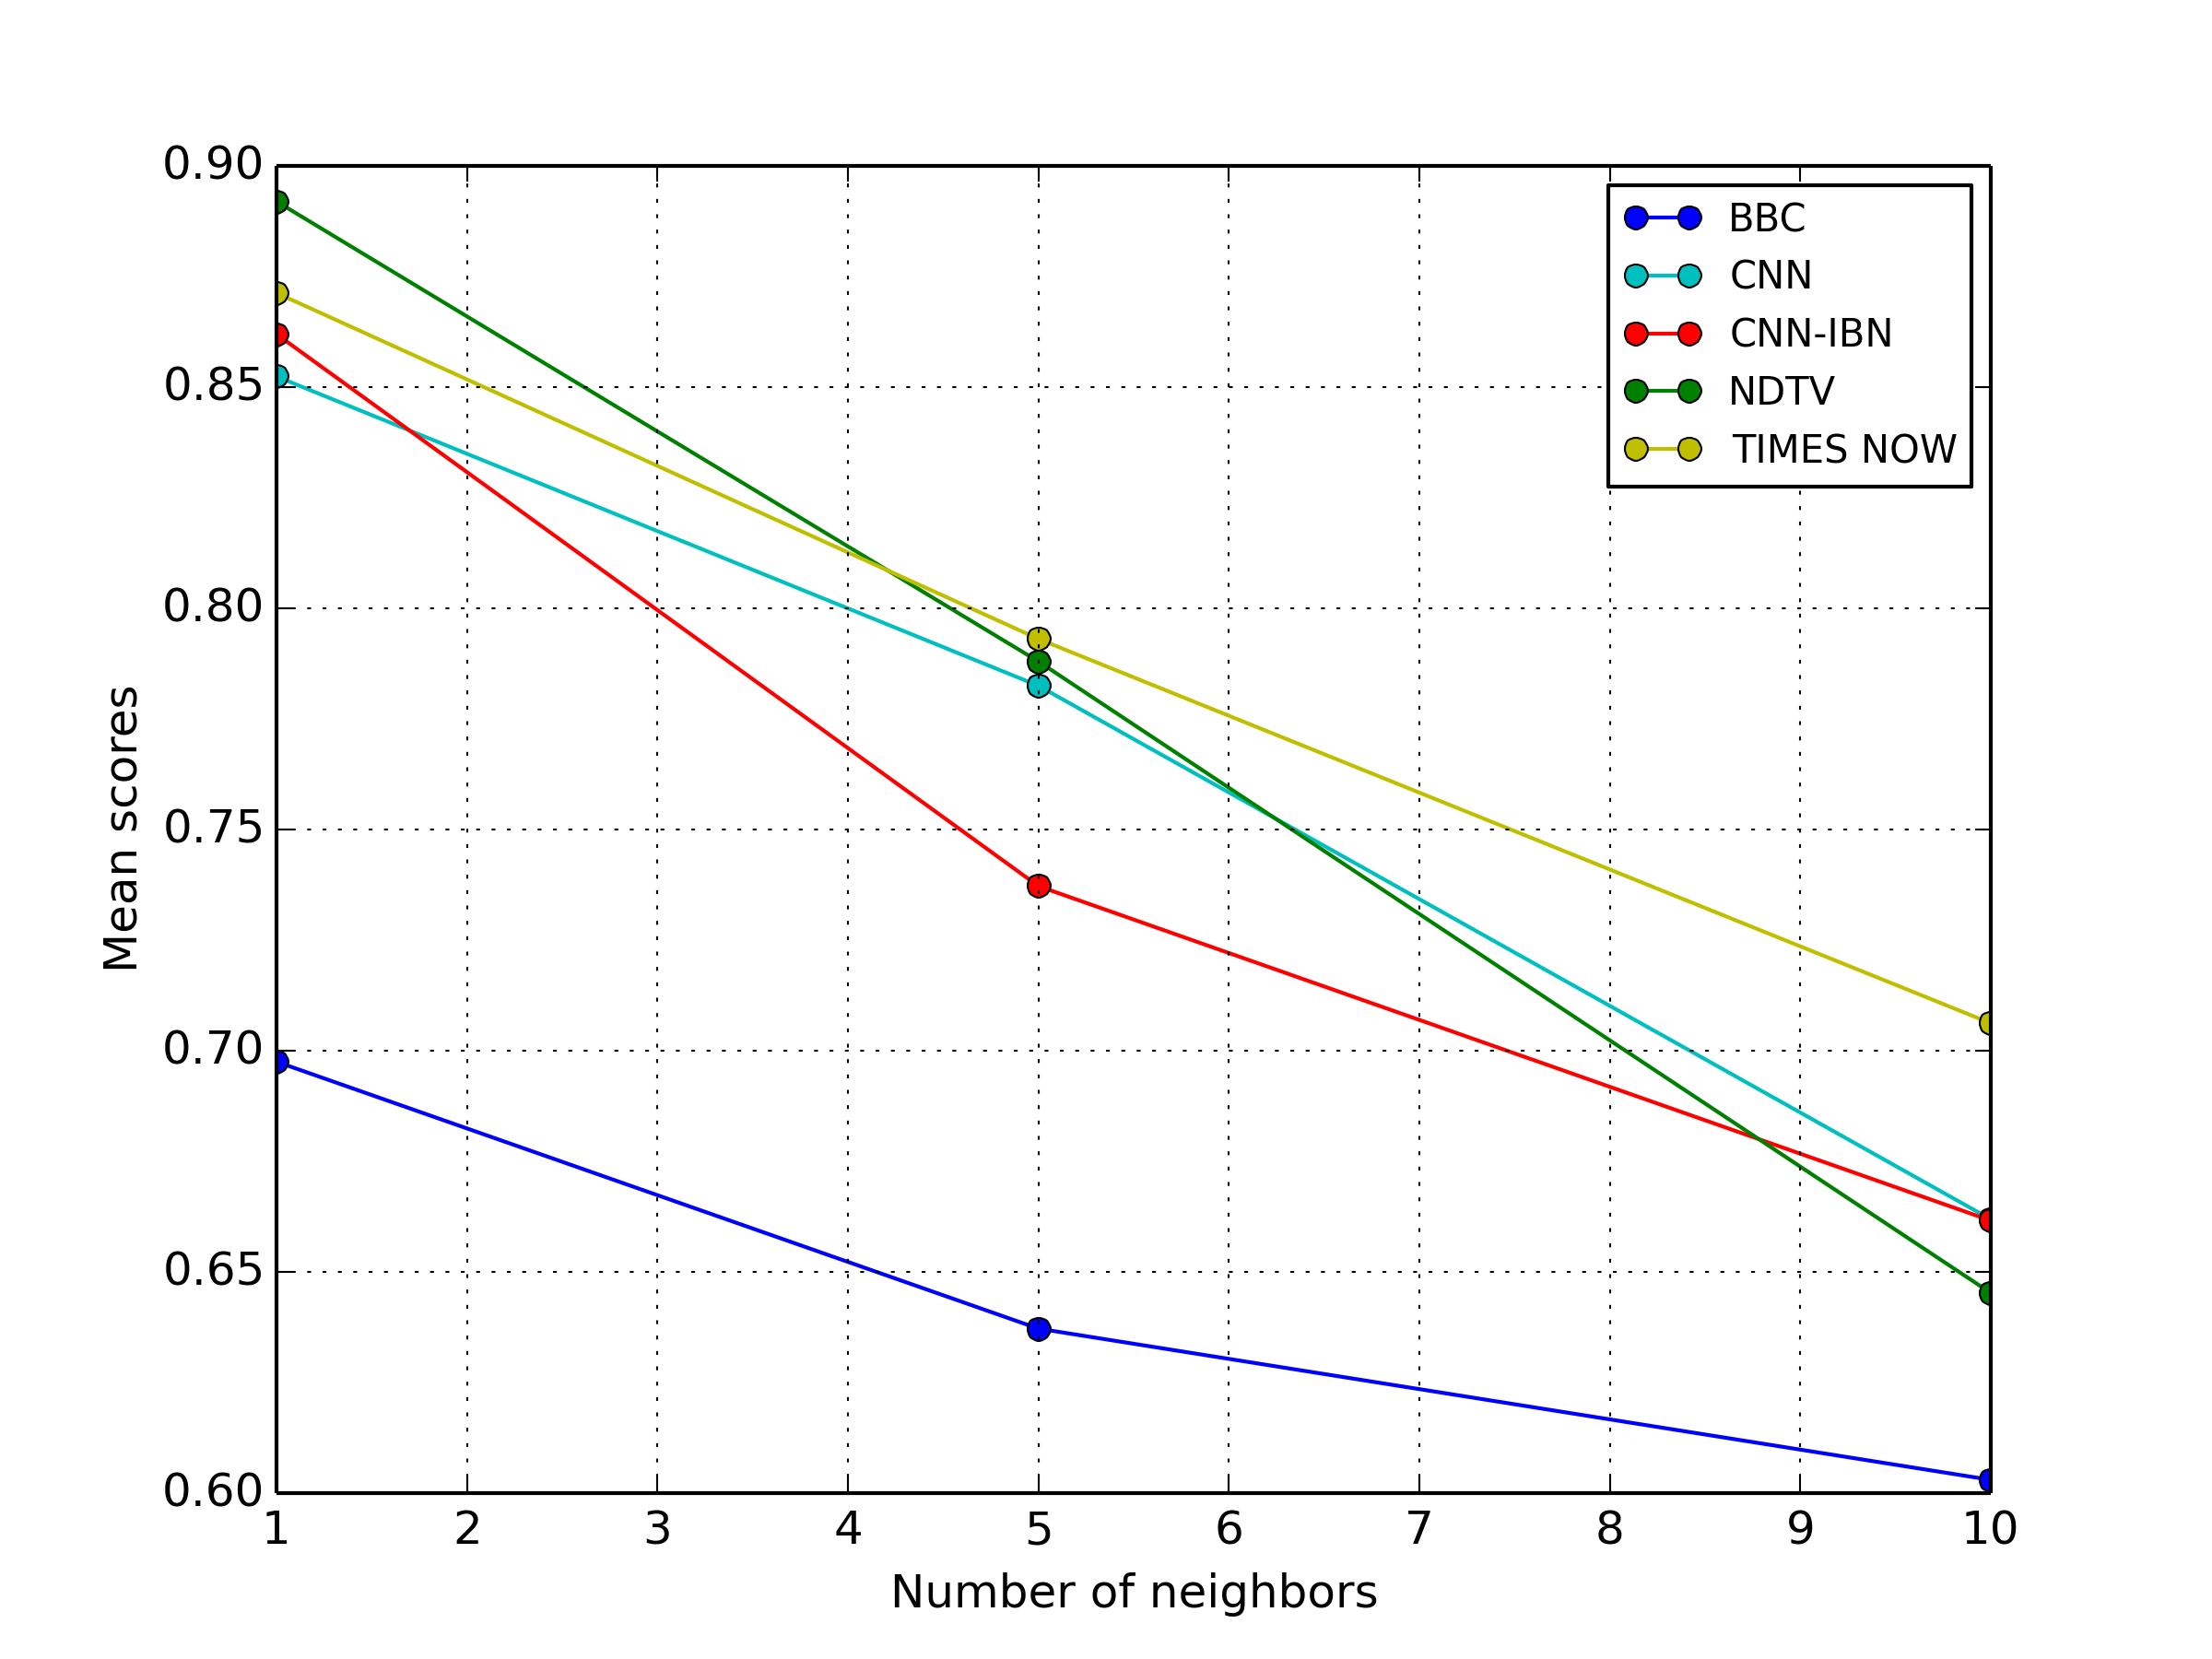
\includegraphics[width=\textwidth]{images/cnn-LDA.png}
		\caption{Качество классификации.}
	\end{subfigure}
	\begin{subfigure}{0.45\textwidth}
		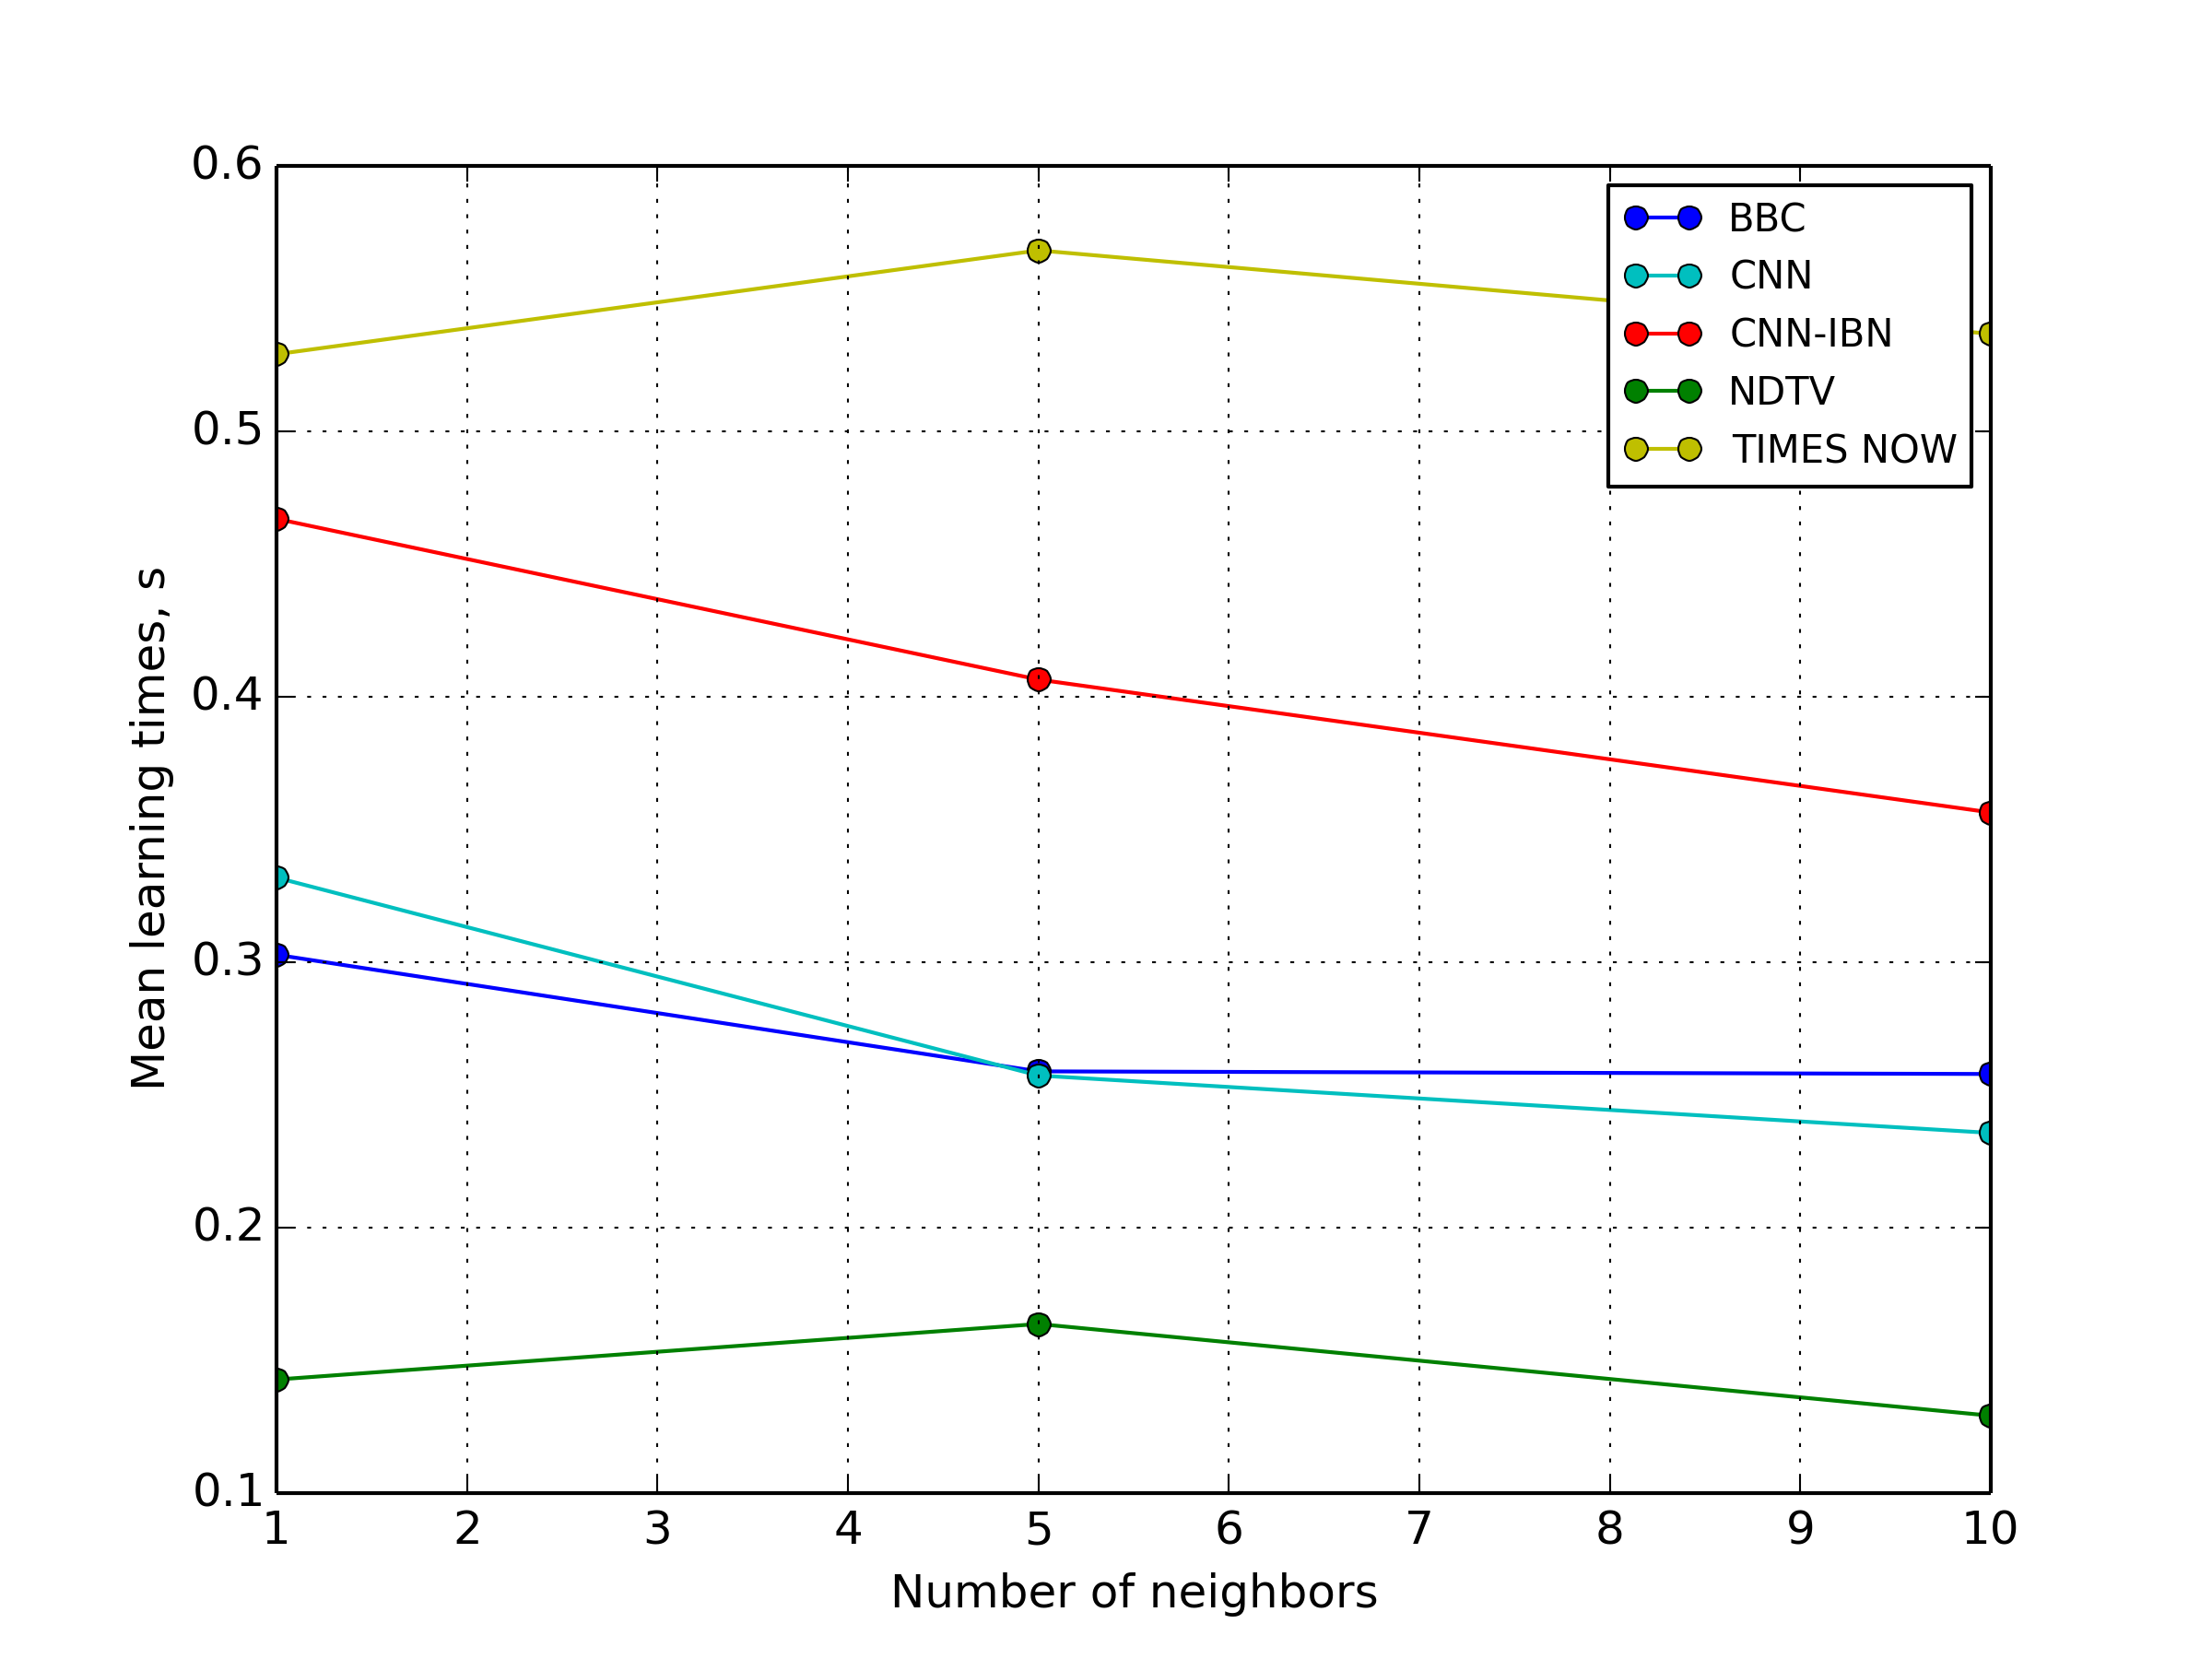
\includegraphics[width=\textwidth]{images/cnn-LDATime.png}
		\caption{Время обучения.}
	\end{subfigure}
	\caption{Результаты применения CNN для LDA.}\label{fig:cnn-lda-results}
\end{figure}

\begin{figure}[h!]
	\centering
	\begin{subfigure}{0.45\textwidth}
		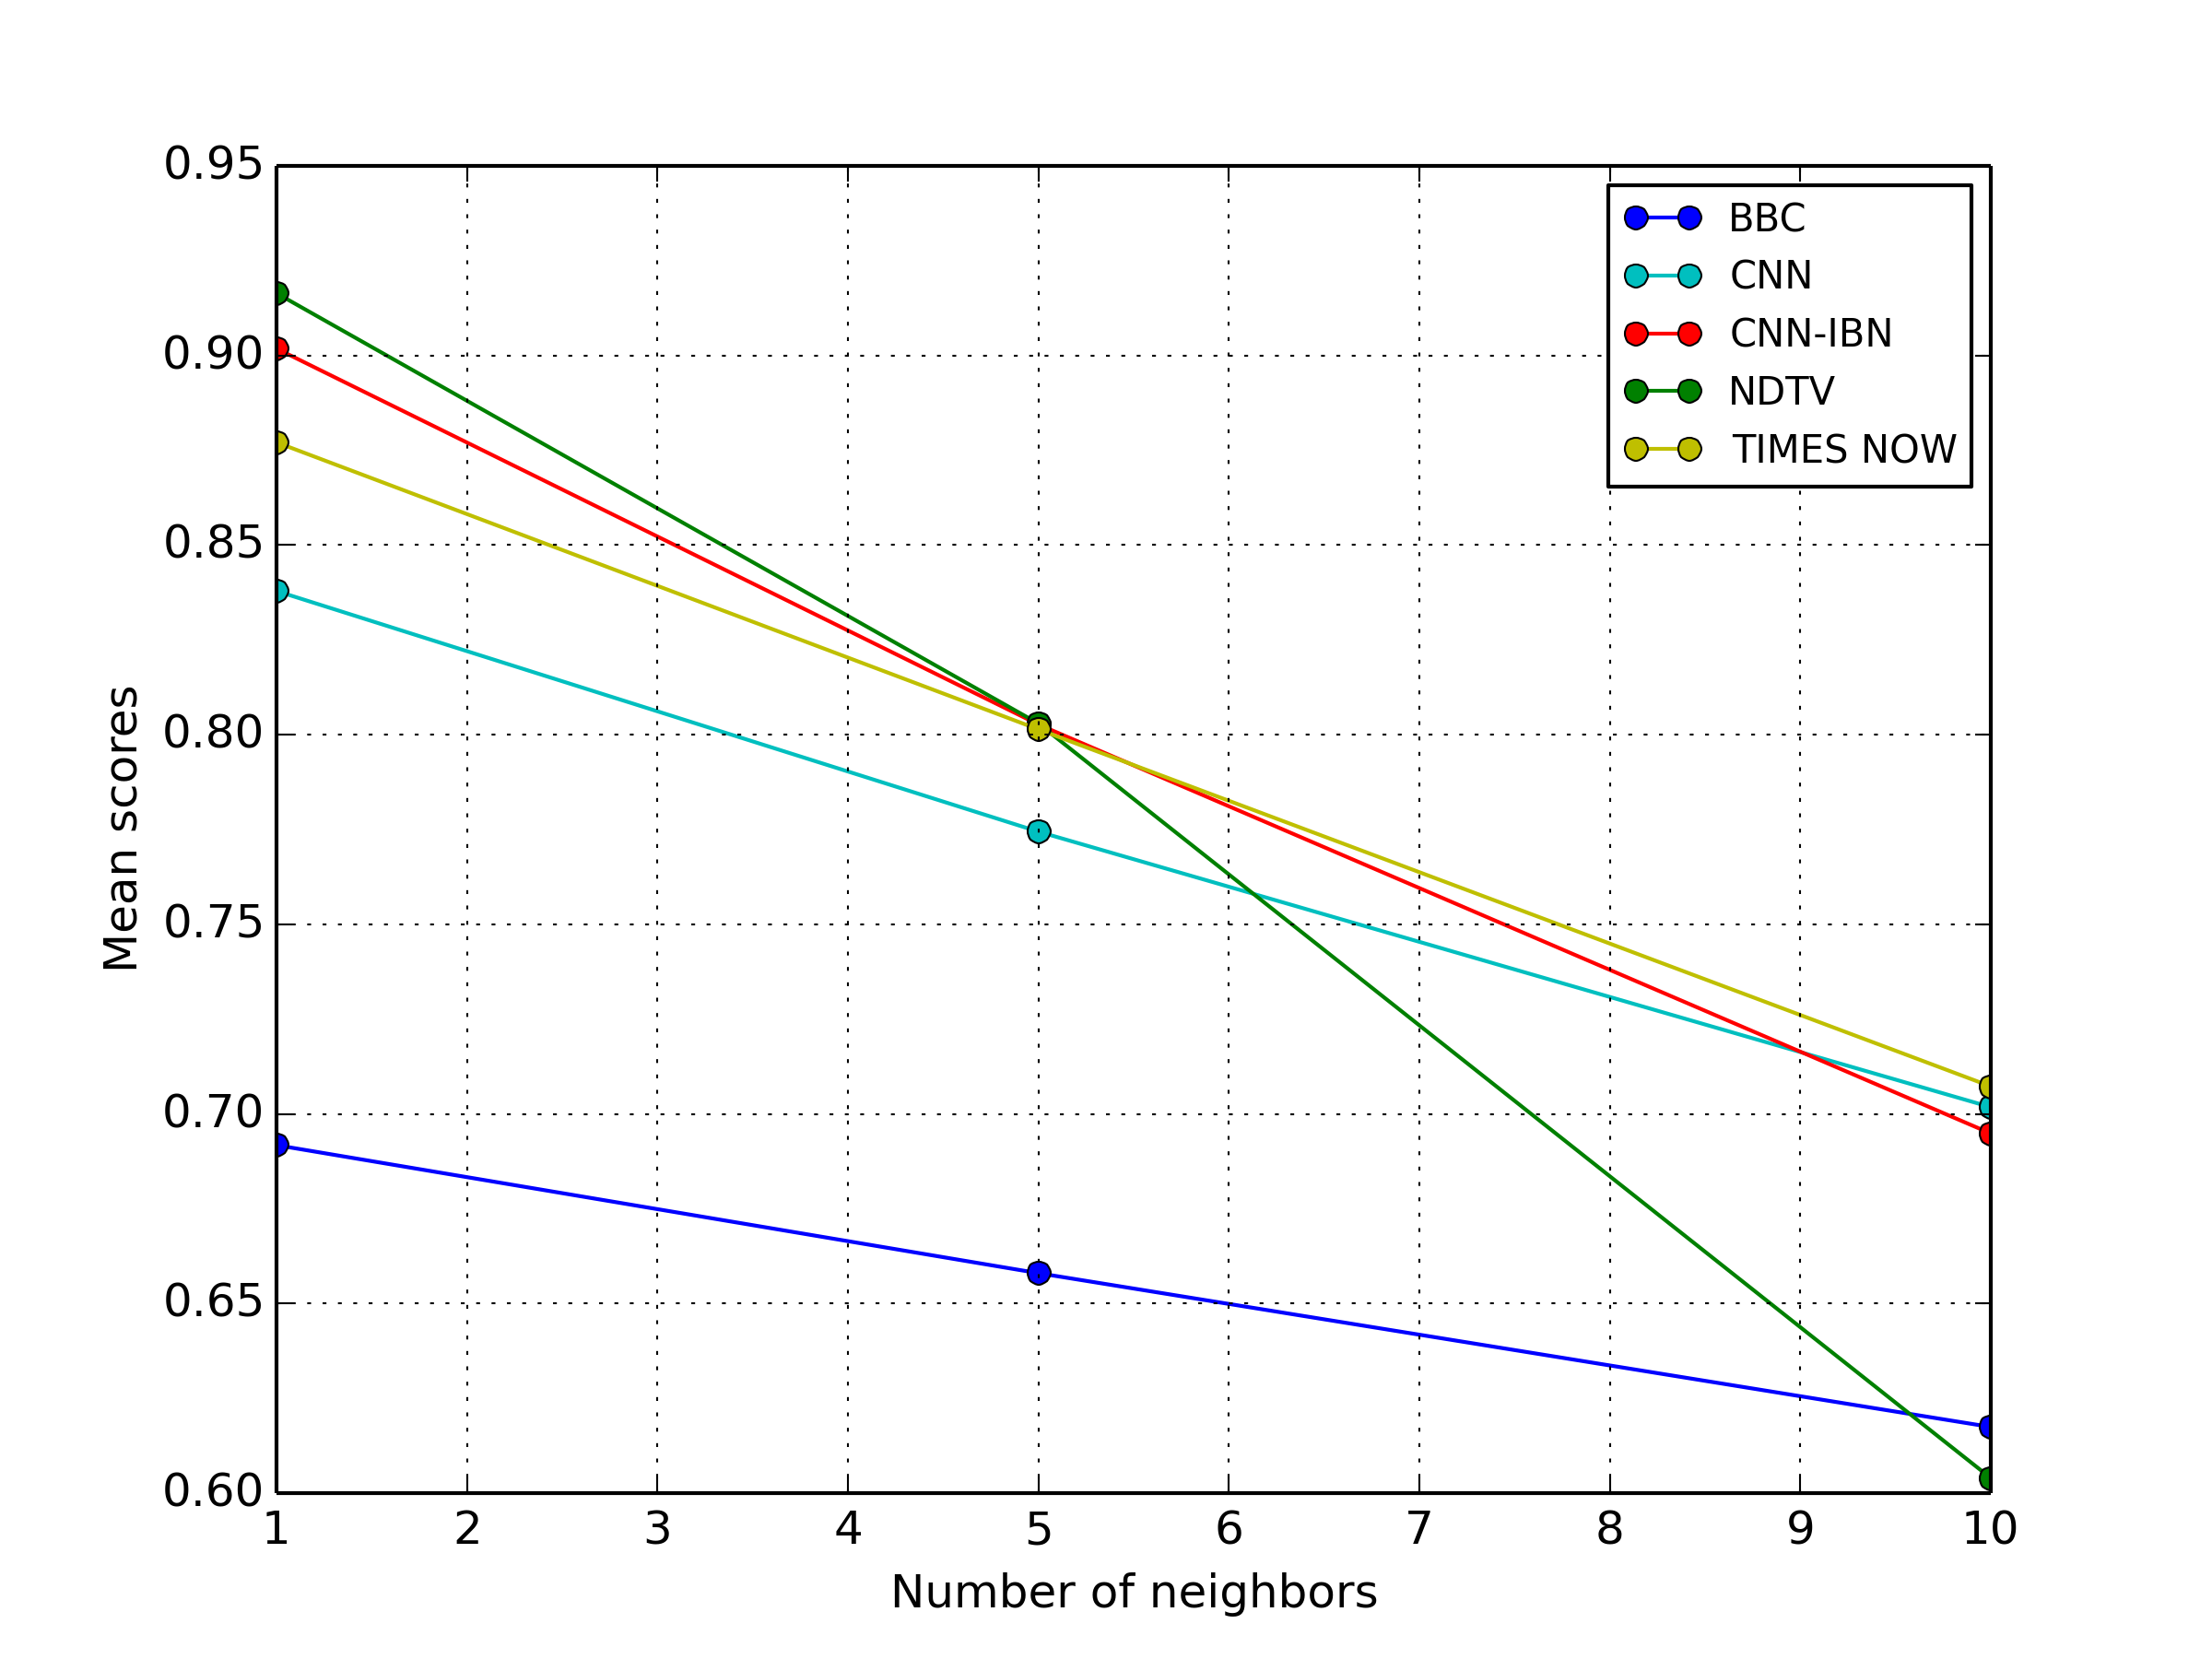
\includegraphics[width=\textwidth]{images/cnn-SVM.png}
		\caption{Качество классификации.}
	\end{subfigure}
	\begin{subfigure}{0.45\textwidth}
		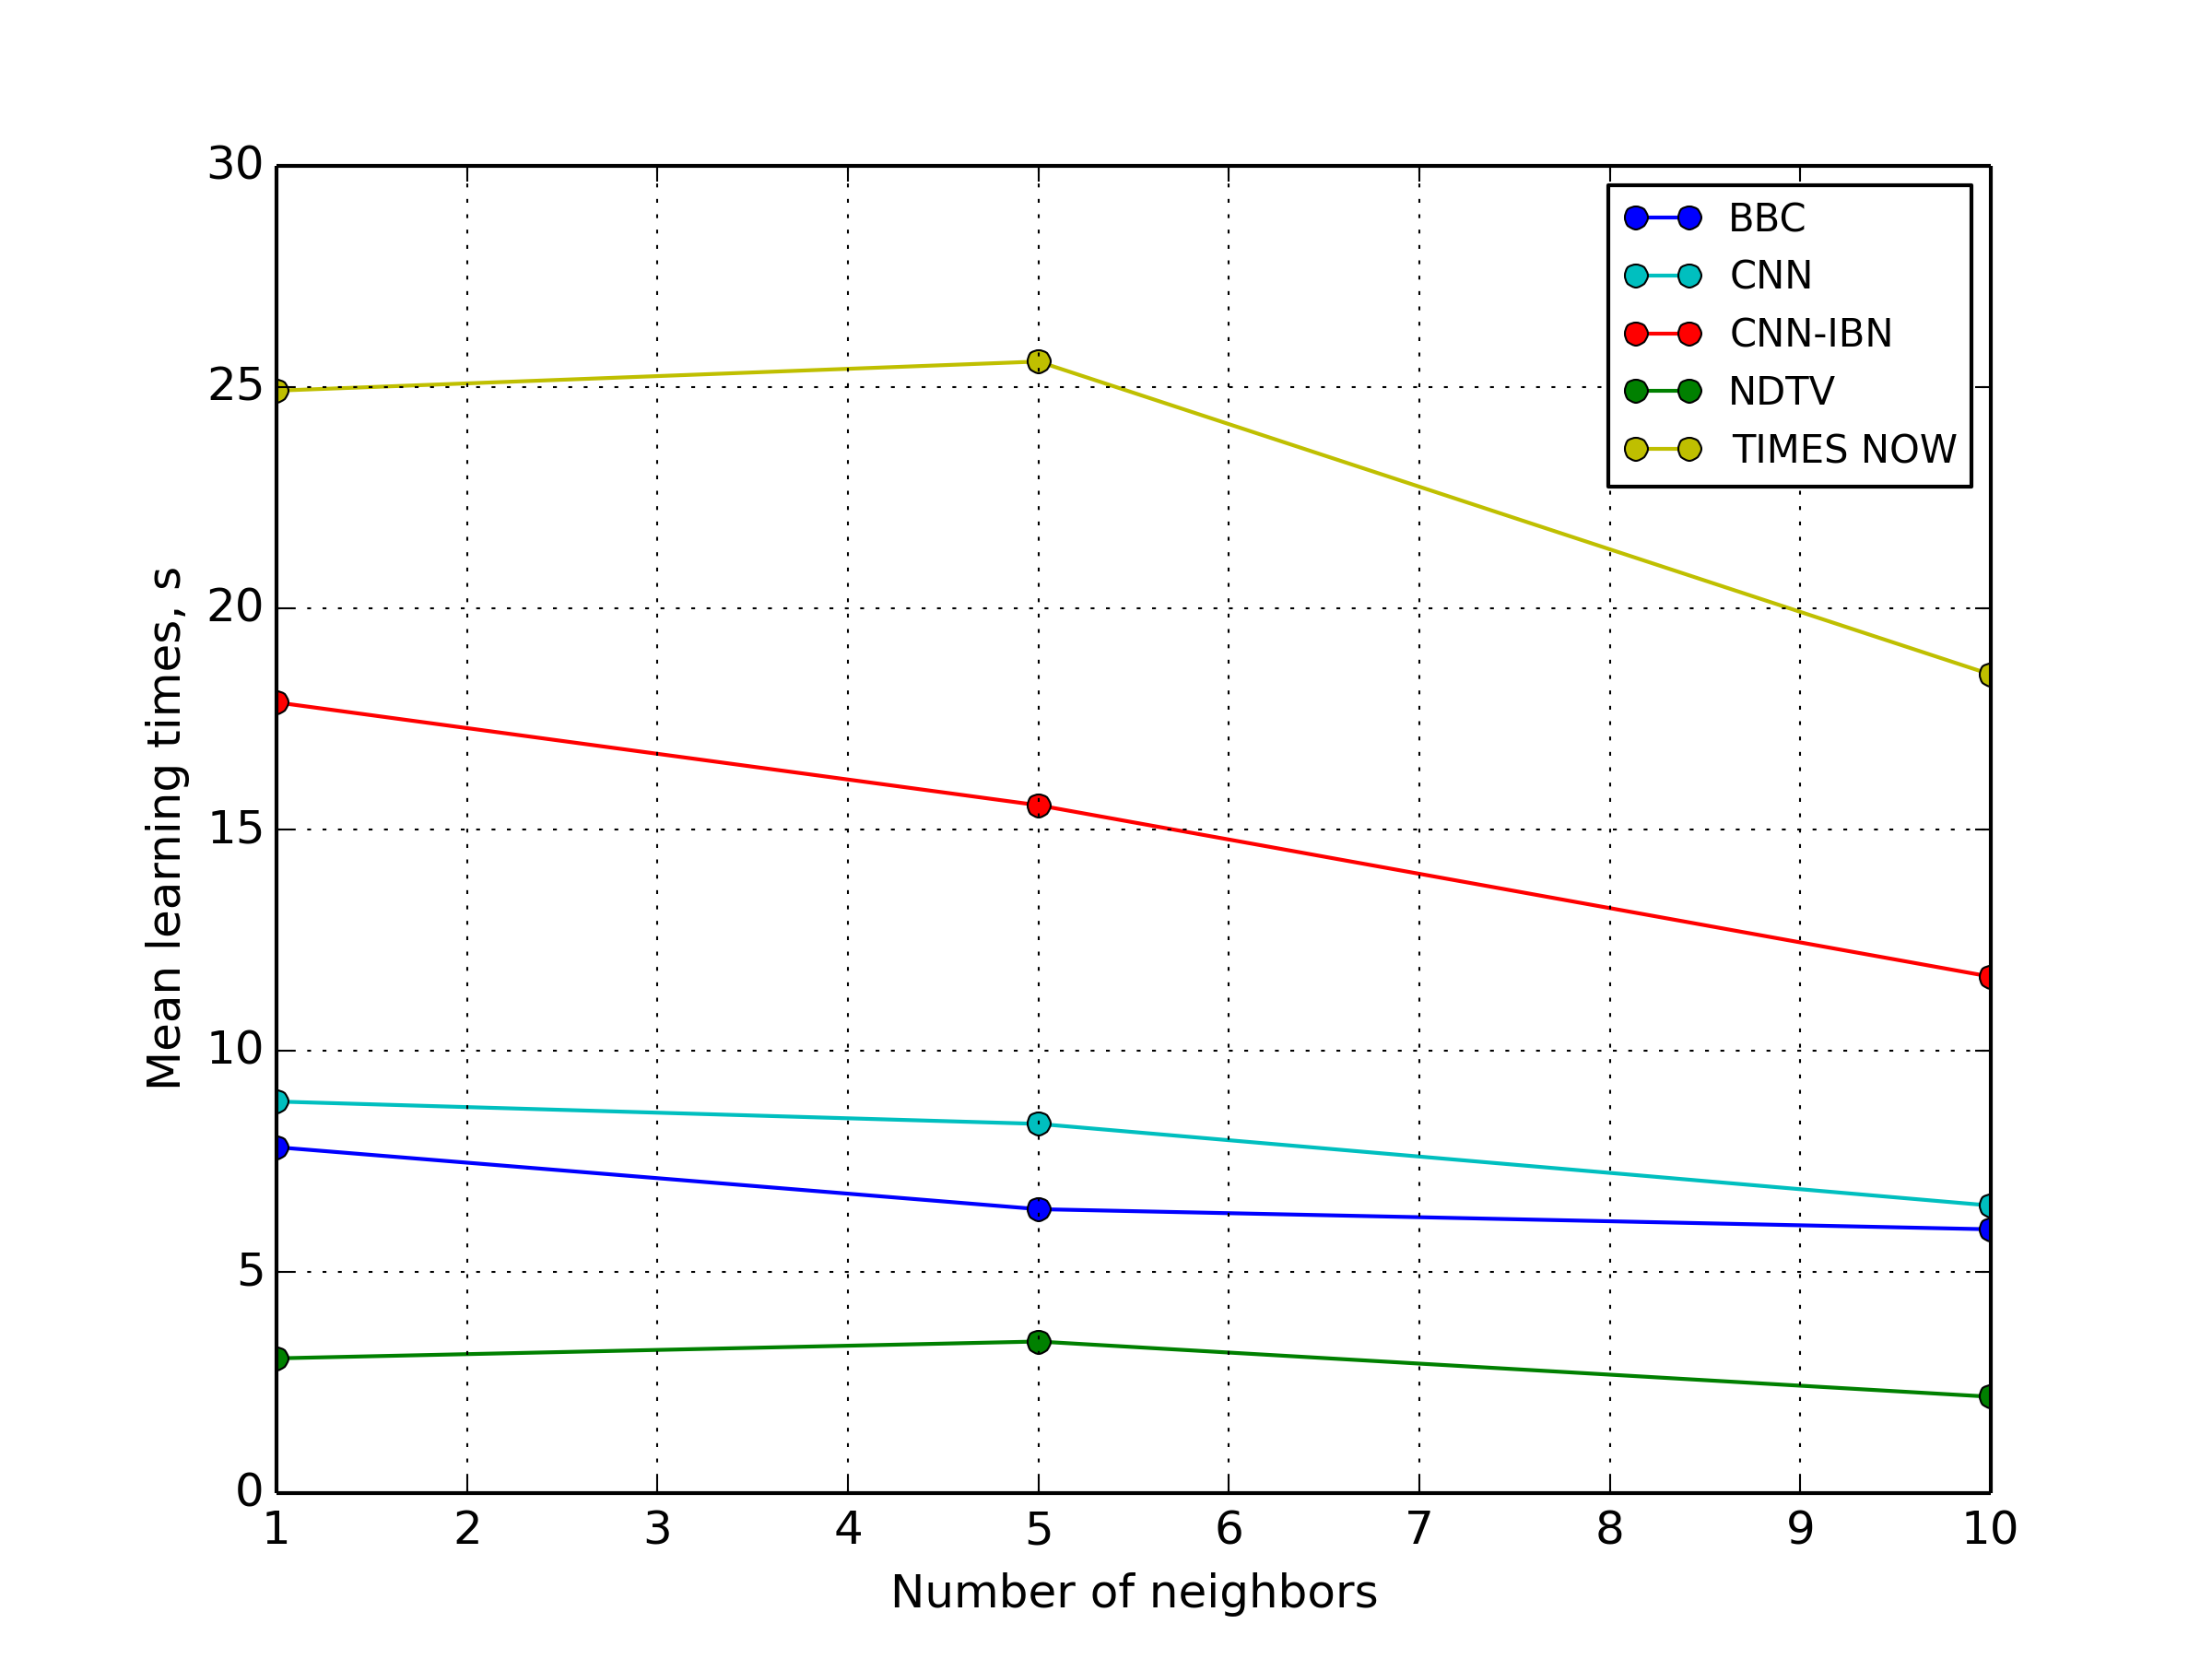
\includegraphics[width=\textwidth]{images/cnn-SVMTime.png}
		\caption{Время обучения.}
	\end{subfigure}
	\caption{Результаты применения CNN для SVM.}\label{fig:cnn-svm-results}
\end{figure}

\begin{figure}[h!]
	\centering
	\begin{subfigure}{0.45\textwidth}
		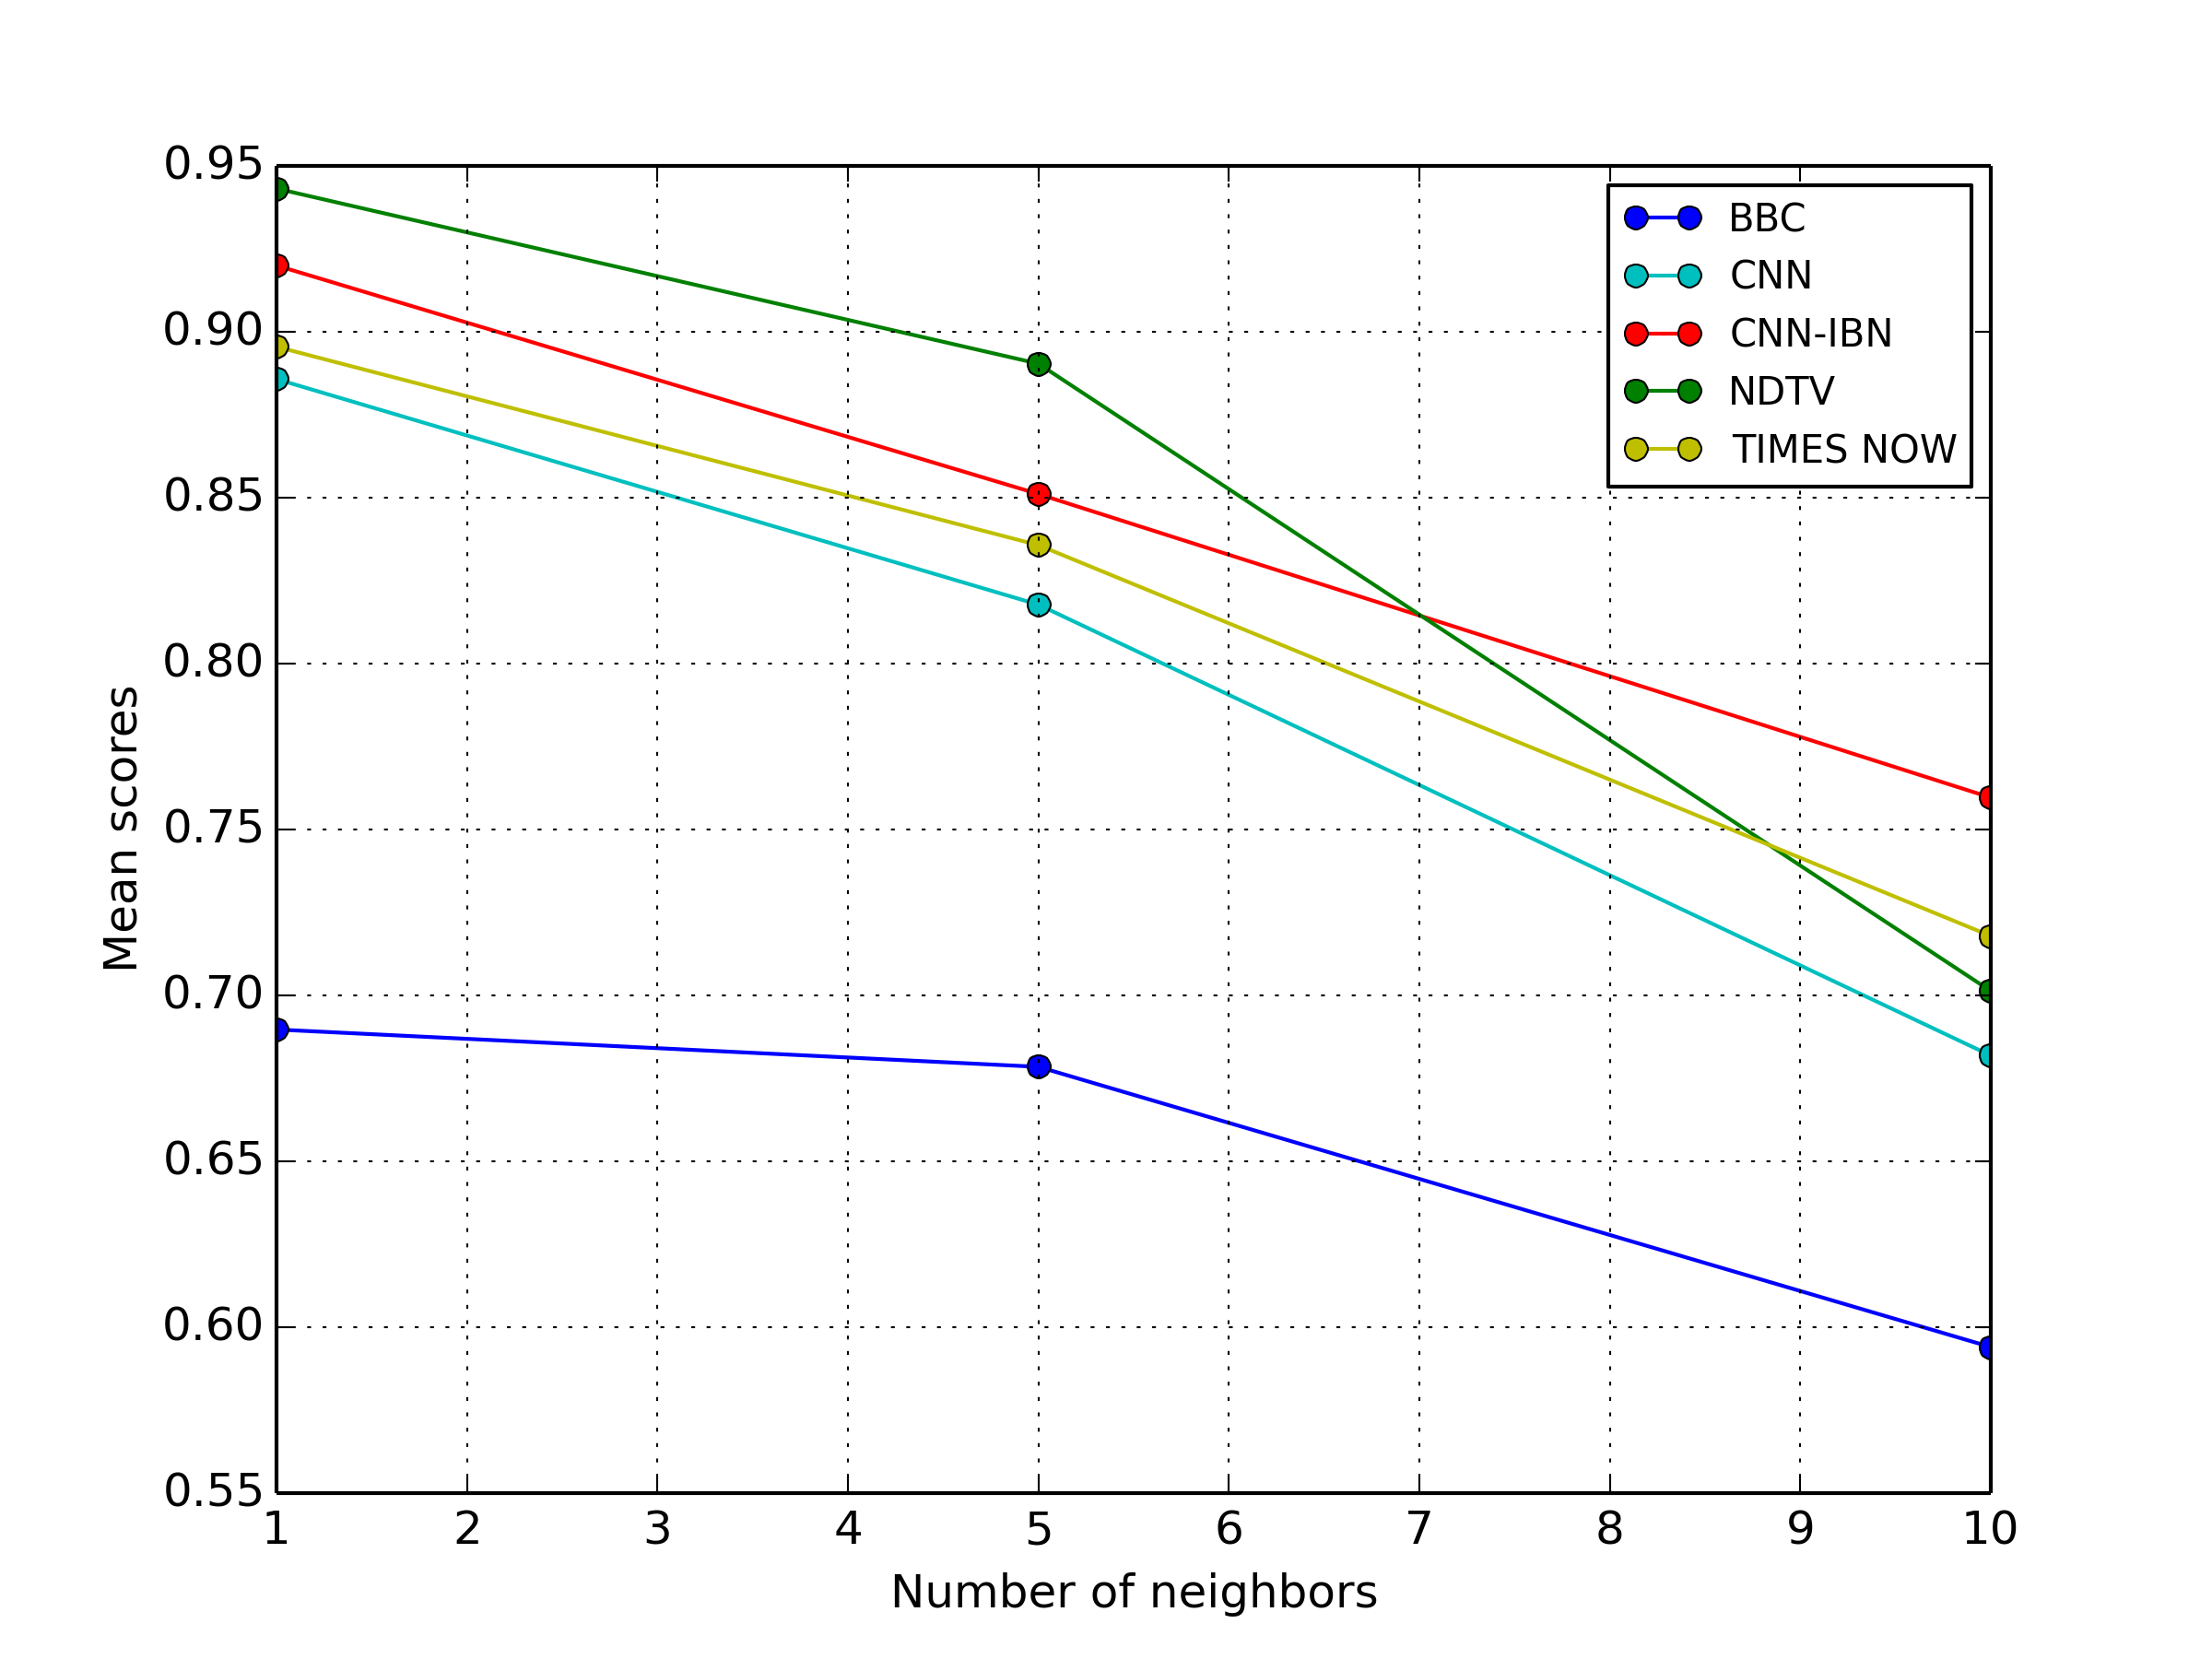
\includegraphics[width=\textwidth]{images/cnn-randforest.png}
		\caption{Качество классификации.}
	\end{subfigure}
	\begin{subfigure}{0.45\textwidth}
		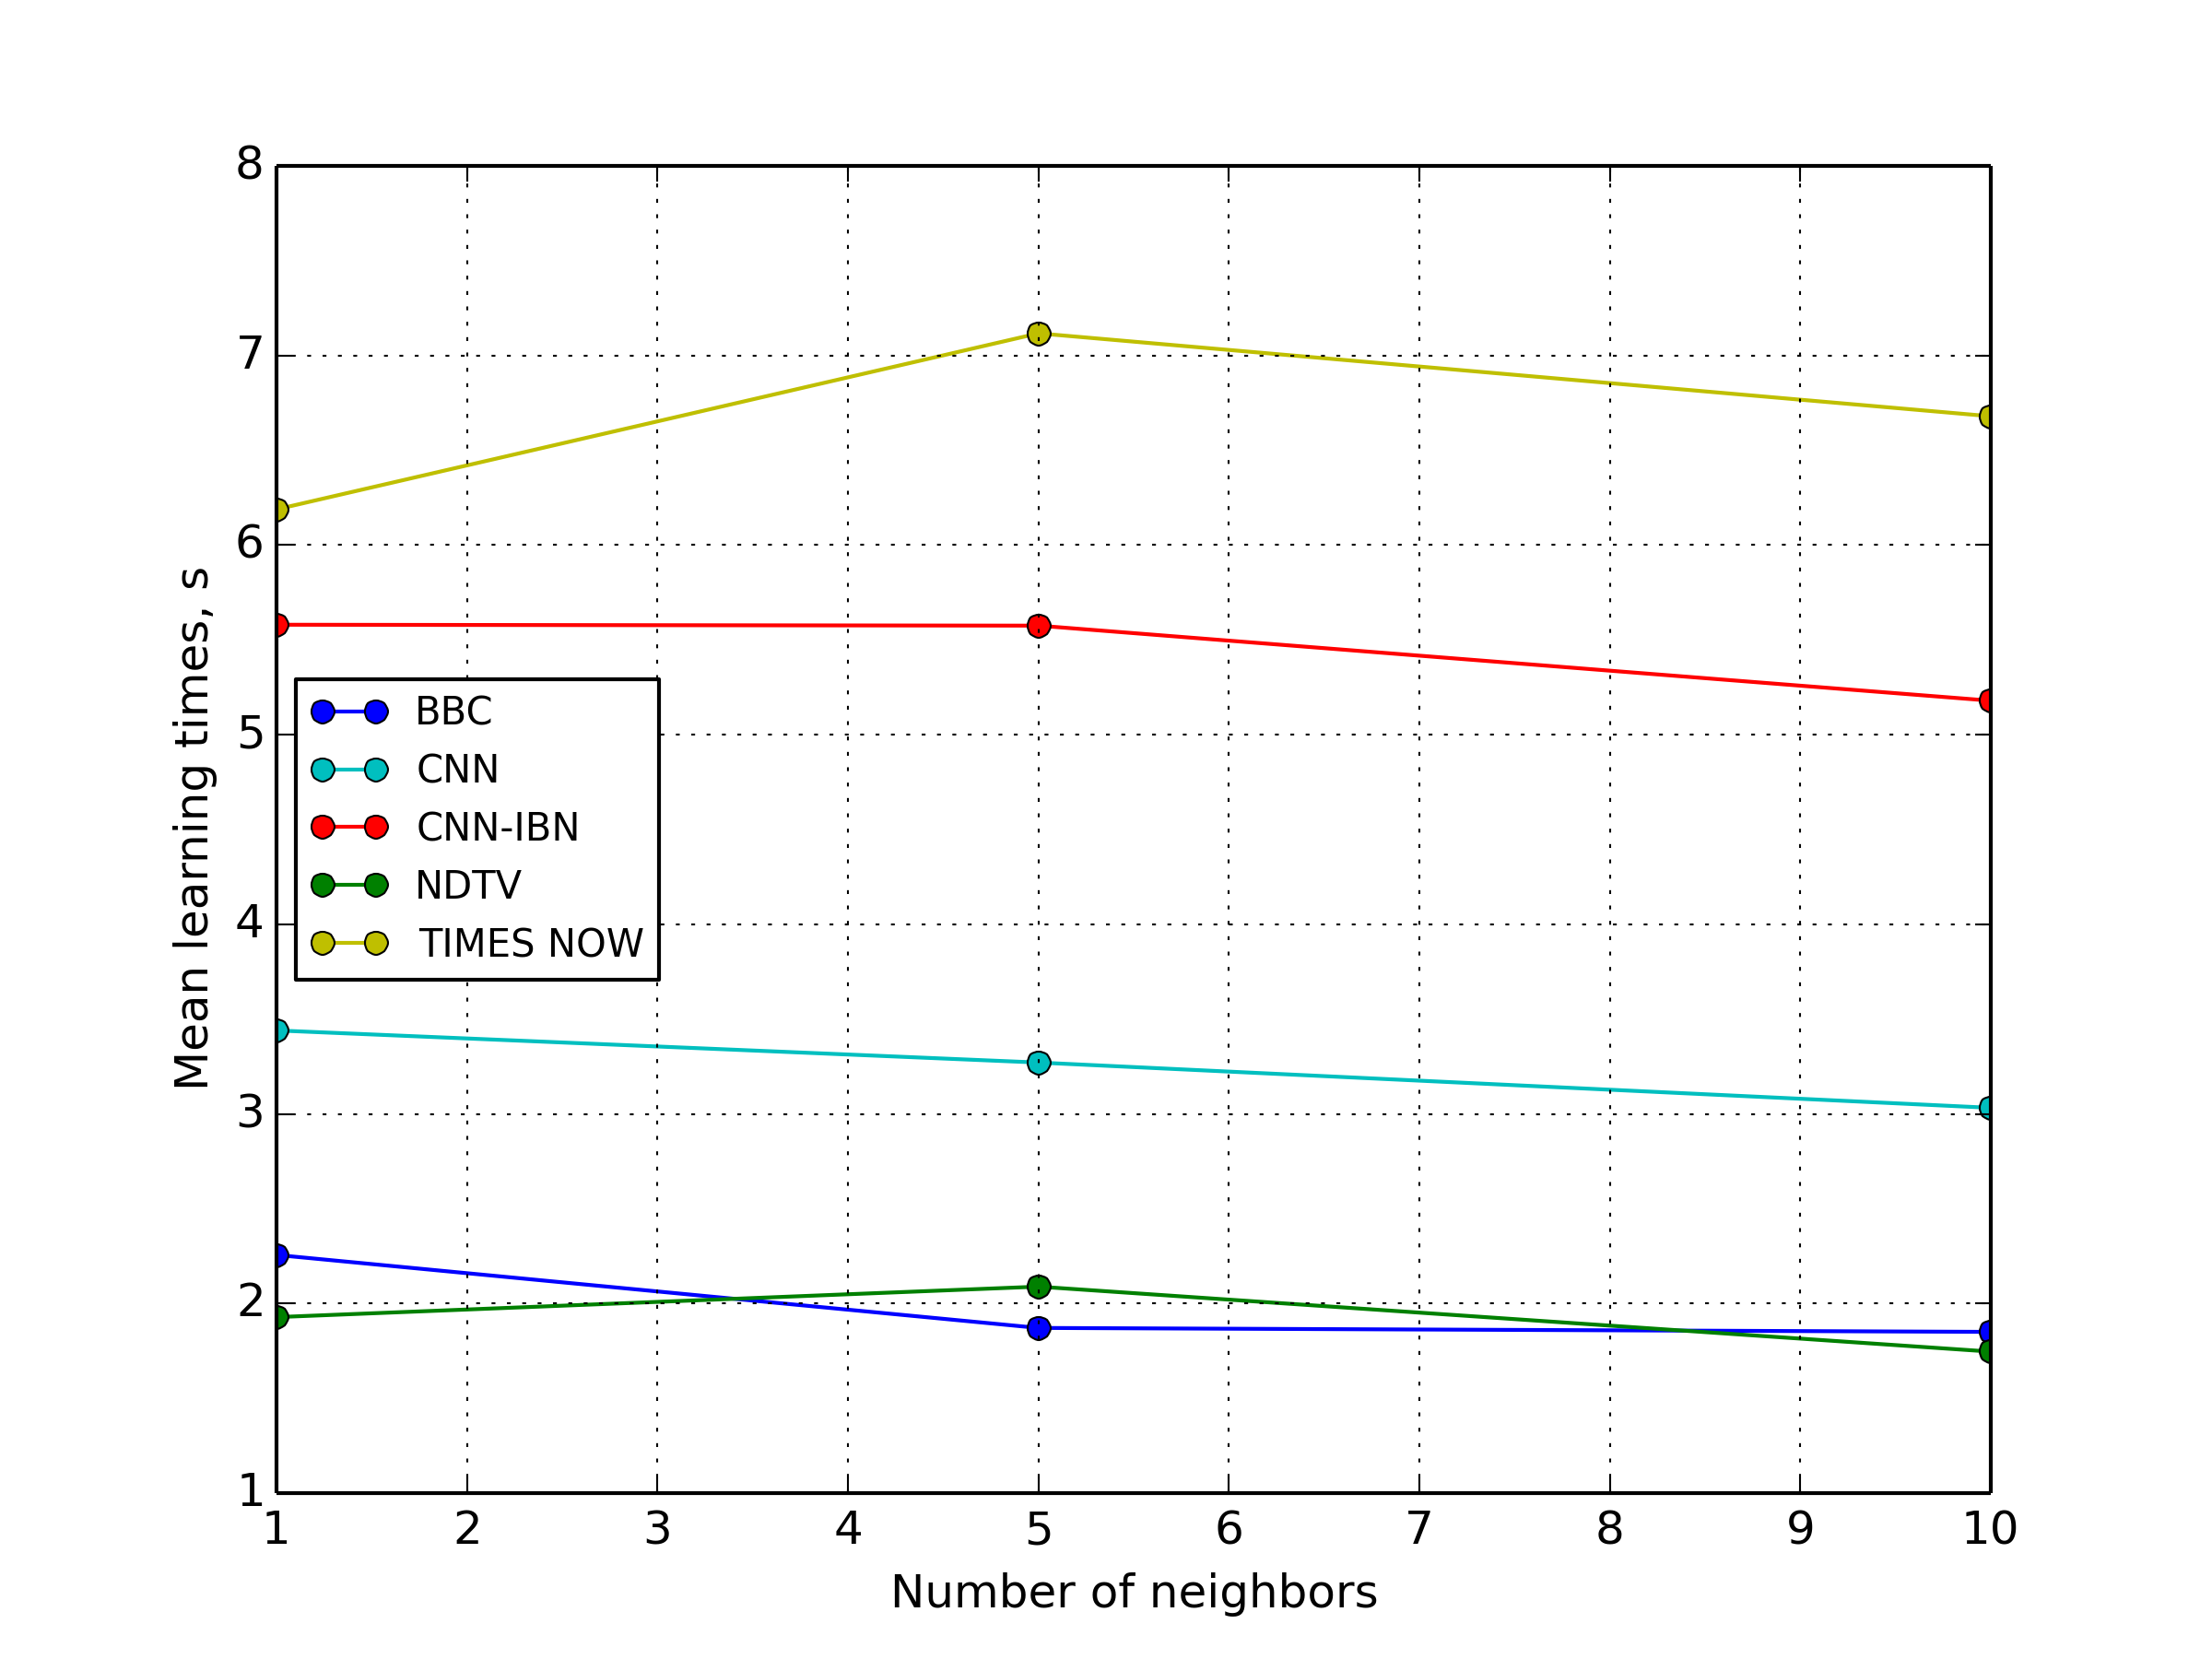
\includegraphics[width=\textwidth]{images/cnn-randforestTime.png}
		\caption{Время обучения.}
	\end{subfigure}
	\caption{Результаты применения CNN для Random forest.}\label{fig:cnn-rf-results}
\end{figure}

\begin{figure}
	\centering
	\begin{subfigure}{0.45\textwidth}
		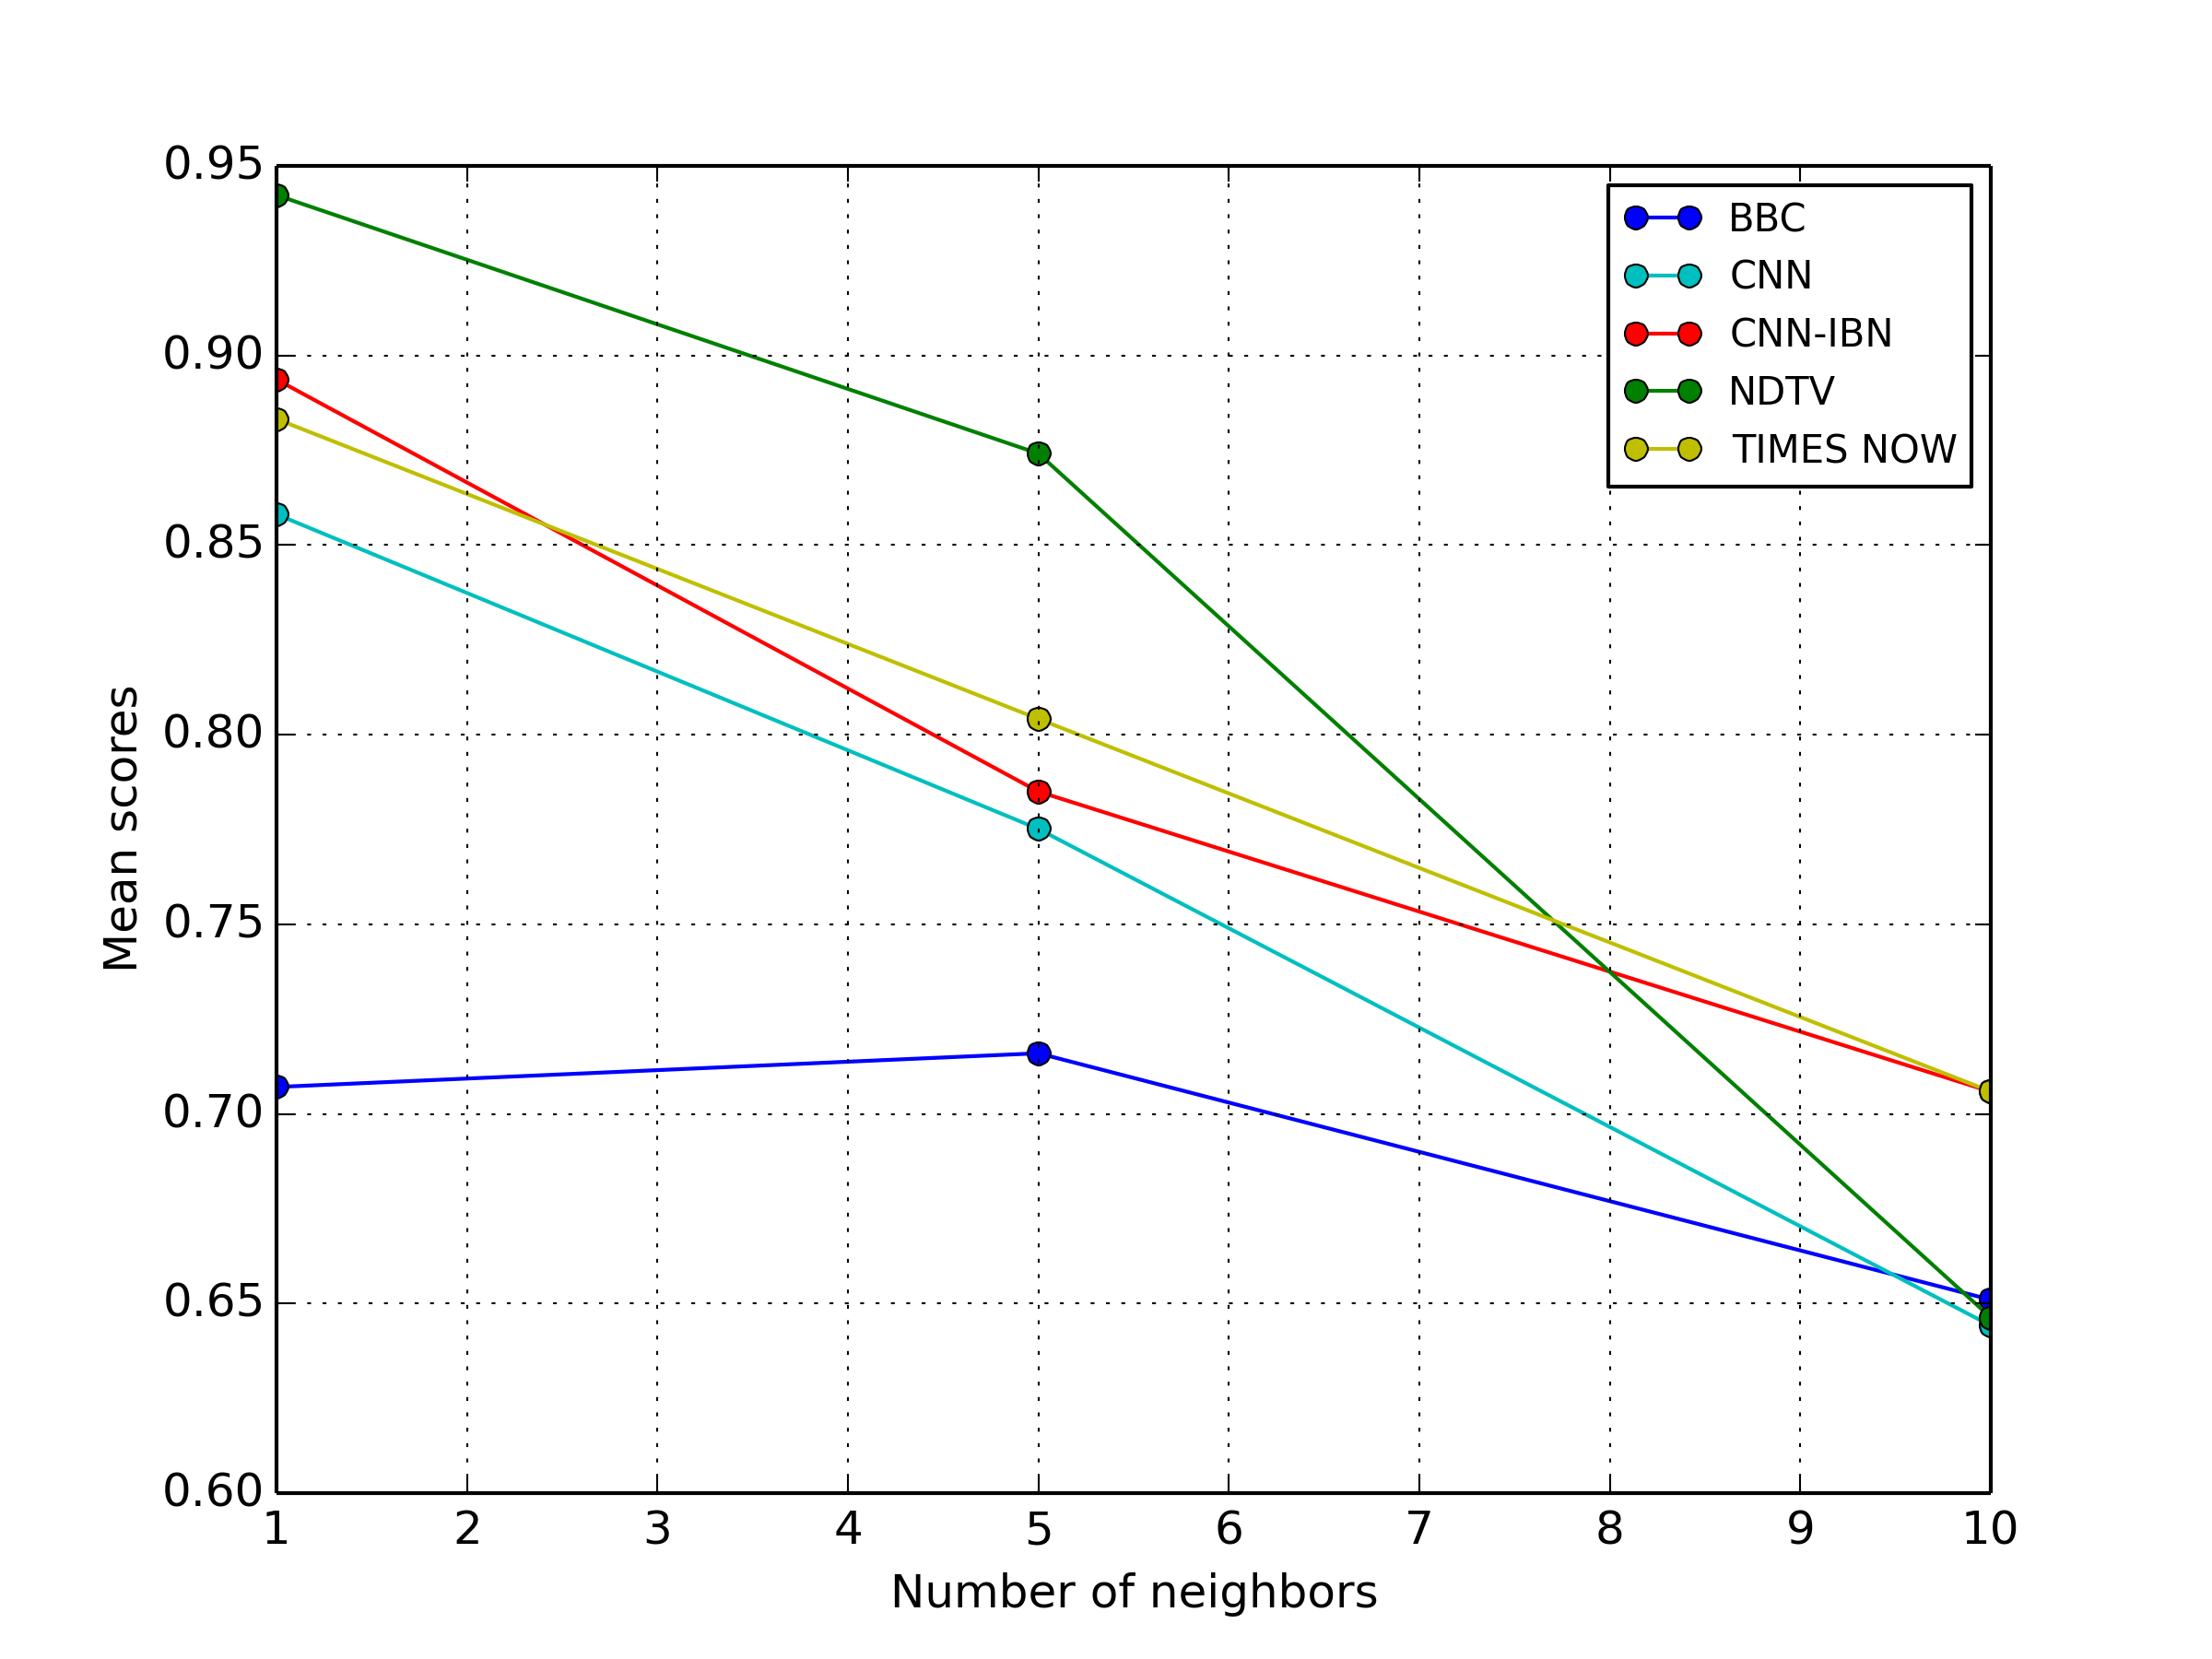
\includegraphics[width=\textwidth]{images/cnn-gradboosting.png}
		\caption{Качество классификации.}
	\end{subfigure}
	\begin{subfigure}{0.45\textwidth}
		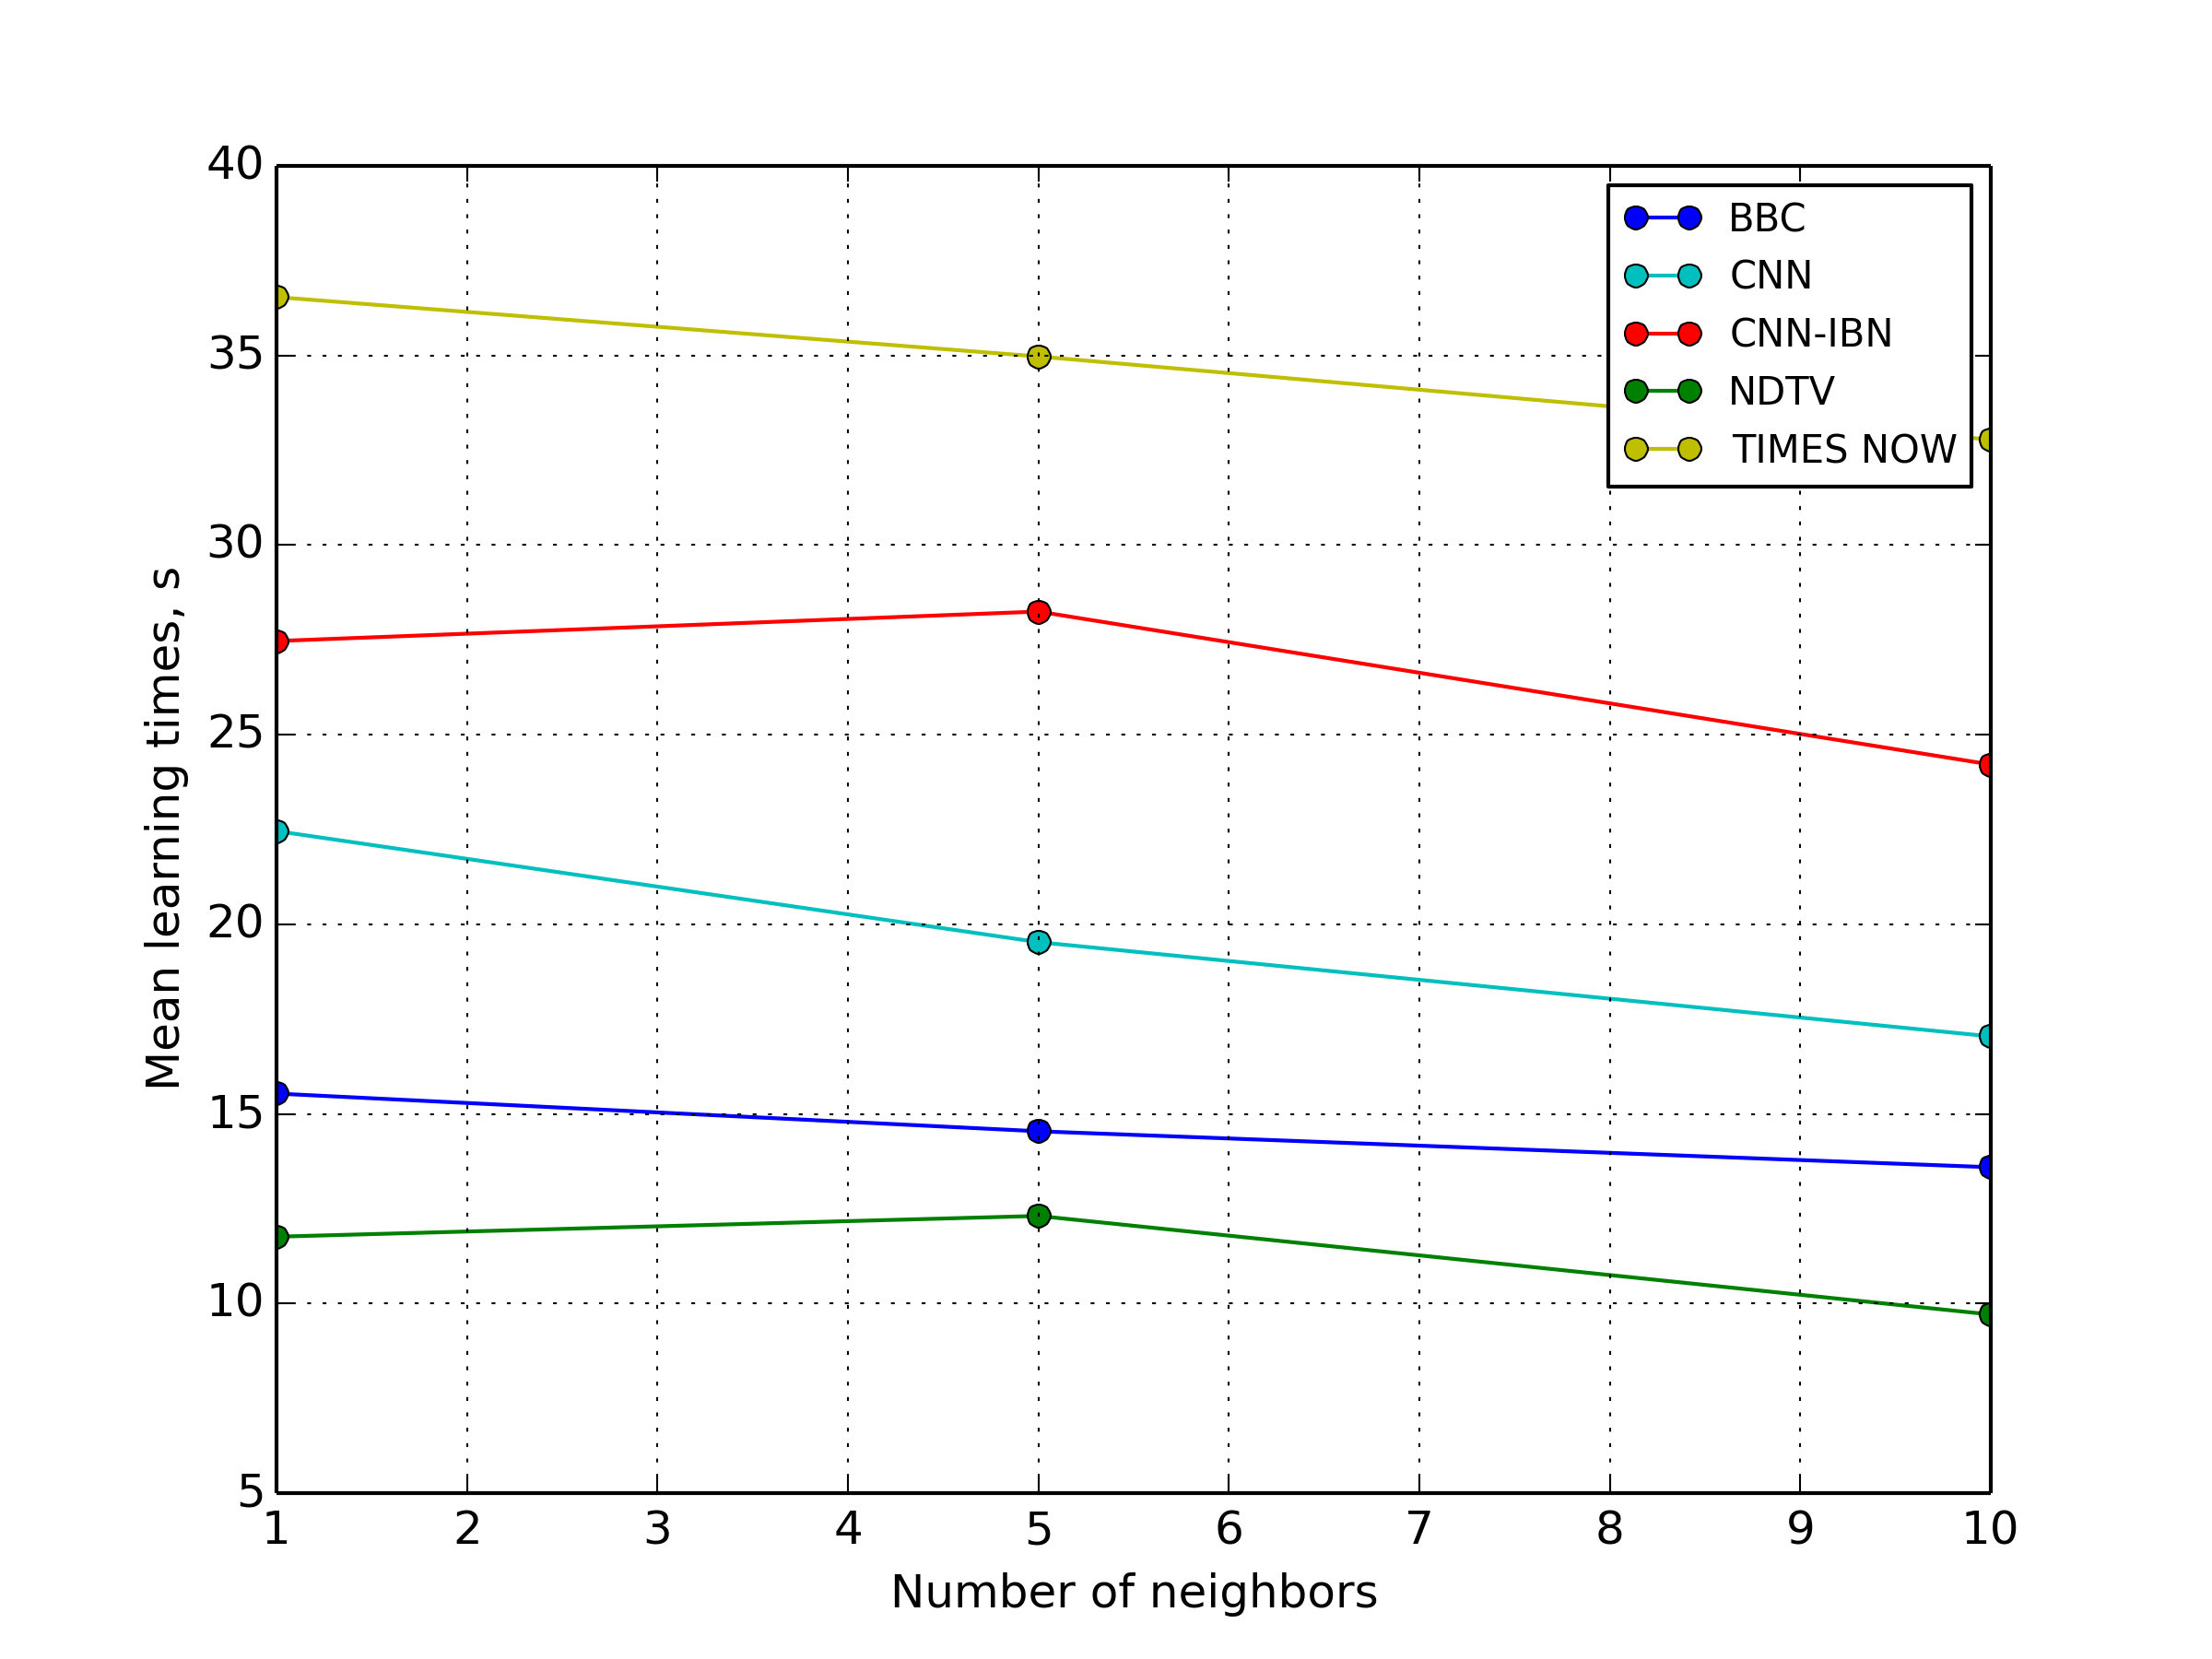
\includegraphics[width=\textwidth]{images/cnn-gradboostingTime.png}
		\caption{Время обучения.}
	\end{subfigure}
	\caption{Результаты применения CNN для GTB}\label{fig:cnn-gtb-results}
\end{figure}

В таблице~\ref{table:cnn-results} приведены результаты применения метода CNN при \(k=1\), как наиболее эффективного варианта. \(R\) и \(T_{PS}\) обозначены процент объектов выборки, оставленный методом CNN, и время работы CNN, соответственно. Как и в таблице~\ref{table:base-all}, \(Q\) означает качество классификации (в скобках указано абсолютное значение, на которое \(Q\) изменилось по сравнению с соответствующим значением в таблице~\ref{table:base-all}), и \(T_{tr}\) означает время обучения (в скобках указано во сколько раз время обучения после редукции больше времени обучения на всей выборке).
\begin{table}[h!]
    \centering
    \begin{tabular}{|c||c||c|c|}
    \cline{2-4}
    \multicolumn{1}{c||}{} & Сжатие \(T\) & \(k\)NN & LDA \\
    \hline \hline
	\input{cnn-table1.txt}
\end{tabular}
\newline \vspace*{0.5cm} \newline
\begin{tabular}{|c||c|c|c|}
    \cline{2-4}
    \multicolumn{1}{c||}{} & SVM & Random forest & GTB \\
    \hline \hline
	\input{cnn-table2.txt}
    \end{tabular}
    \caption{Сводная таблица результатов метода CNN и базовых методов после применения CNN}
    \label{table:cnn-results}
\end{table}

\tbd{Обновить} Из таблицы~\ref{table:cnn-results} видно, что метод CNN на всех каналах добился значительного сокращения обучающей выборки (от \(\frac23\) до \(\frac34\)). На редуцированной выборке метод 13 ближайших соседей стал работать намного быстрее (хотя на представленных наборах данных он и без редукции работал быстро), но его точность сильно пострадала. Линейный дискриминантный анализ также не получил большой пользы от выбора эталонов. С другой стороны, случайный лес сохранил свою точность (на каналах CNN-IBN, TIMESNOW, NDTV) и при этом отработал намного быстрее, чем на полных обучающих выборках.

\subsection{Fast condensed nearest neighbor}
Метод FCNN \cite{angiulli} был предложен с целью исправить некоторые недостатки CNN и других методов, основанных на \(k\)NN: зависимость результирующего подмножества \(S\) от порядка элементов в обучающей выборке и низкая производительность и масштабируемость. Сначала \(S\) содержит точки, ближайшие к барицентрам классов (барицентр класса --- \(\mathbf{x}_C=|C|^{-1}\sum_{c\in C}\mathbf{x}_c\), где \(C\) --- множество индексов обектов, принадлежащих одному классу). Затем, множество \(T\setminus S\) разбивается на \(|S|\) непересекающихся классов \(Vor(p, S, T)\) (так называмые Voronoi cells), в каждом из которых находятся объекты, для которых ближайшим соседом является один и тот же объект \(p\in S\). Затем все объекты из \(T\setminus S\) классифицируются методом ближайшего соседа с обучающей выборкой \(S\) и в каждом \(Vor(p, S, T)\) выбираются неверно классифицированные объекты, которые составляют множества \(Voren(p, S, T)\) (Voronoi enemies). После этого для каждого такого \(p\in S\), что \(Voren(p, S, T)\neq\varnothing\) выбирается ближайший к \(p\) объект из \(Voren(p, S, T)\) и они одновременно добавляются в \(S\). На каждой следующей итерации процедура повторяется для нового \(S\). Алгоритм останавливается, когда на последней итерации в \(S\) не было добавлено ни одного элемента.

FCNN может быть расширен на число ближайших соседей, отличных от 1, аналогично CNN: при классификации объектов в \(T\setminus S\) нужно использовать метод \(k\)NN. В \cite{angiulli} приведено доказательство того, что он строит согласованное подмножество \(S\), одинаковое для любого упорядочивания обучающей выборки.

Аналогично CNN, с FCNN были проведены эксперименты для \(k\in\{1,5,10\}\). Доли отобранных объектов и времена работы для каждого из каналов приведены на рис.~\ref{fig:fcnn-stats}.
\begin{figure}[h!]
    \centering
	\begin{subfigure}{0.45\textwidth}
		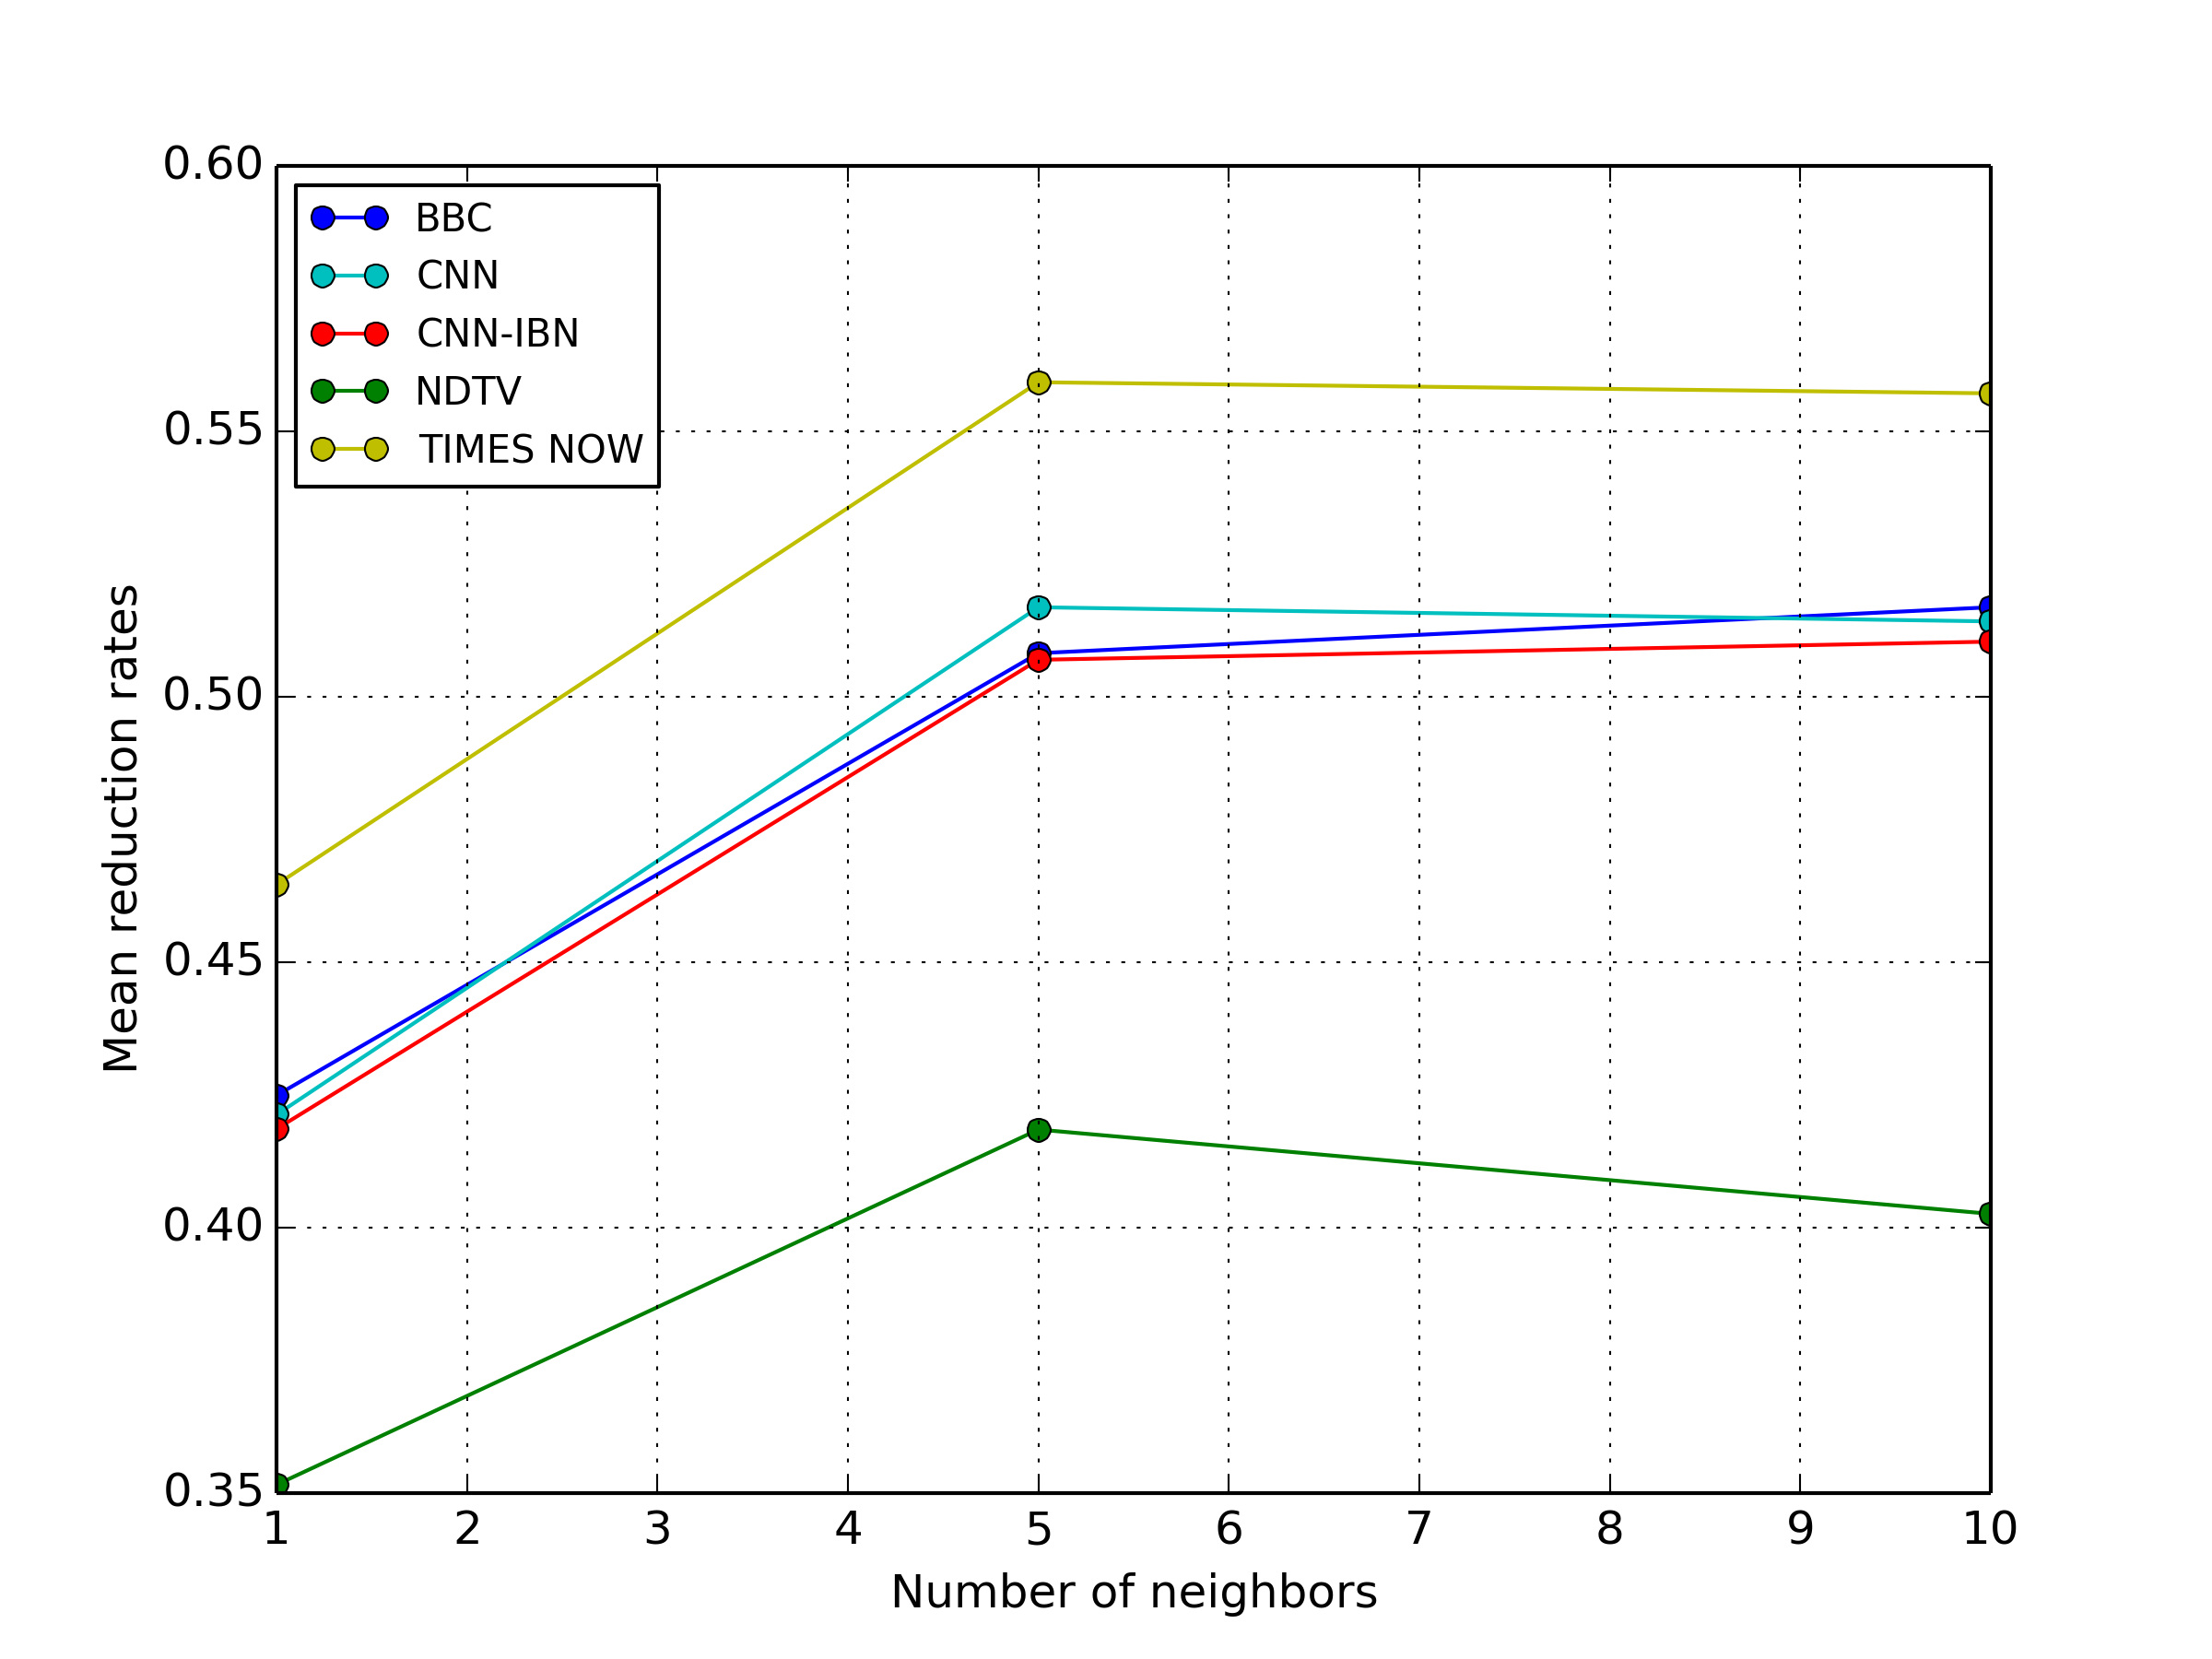
\includegraphics[width=\textwidth]{images/fcnn-stats.png}
		\caption{Доля отобранных объектов.}
	\end{subfigure}
	\begin{subfigure}{0.45\textwidth}
		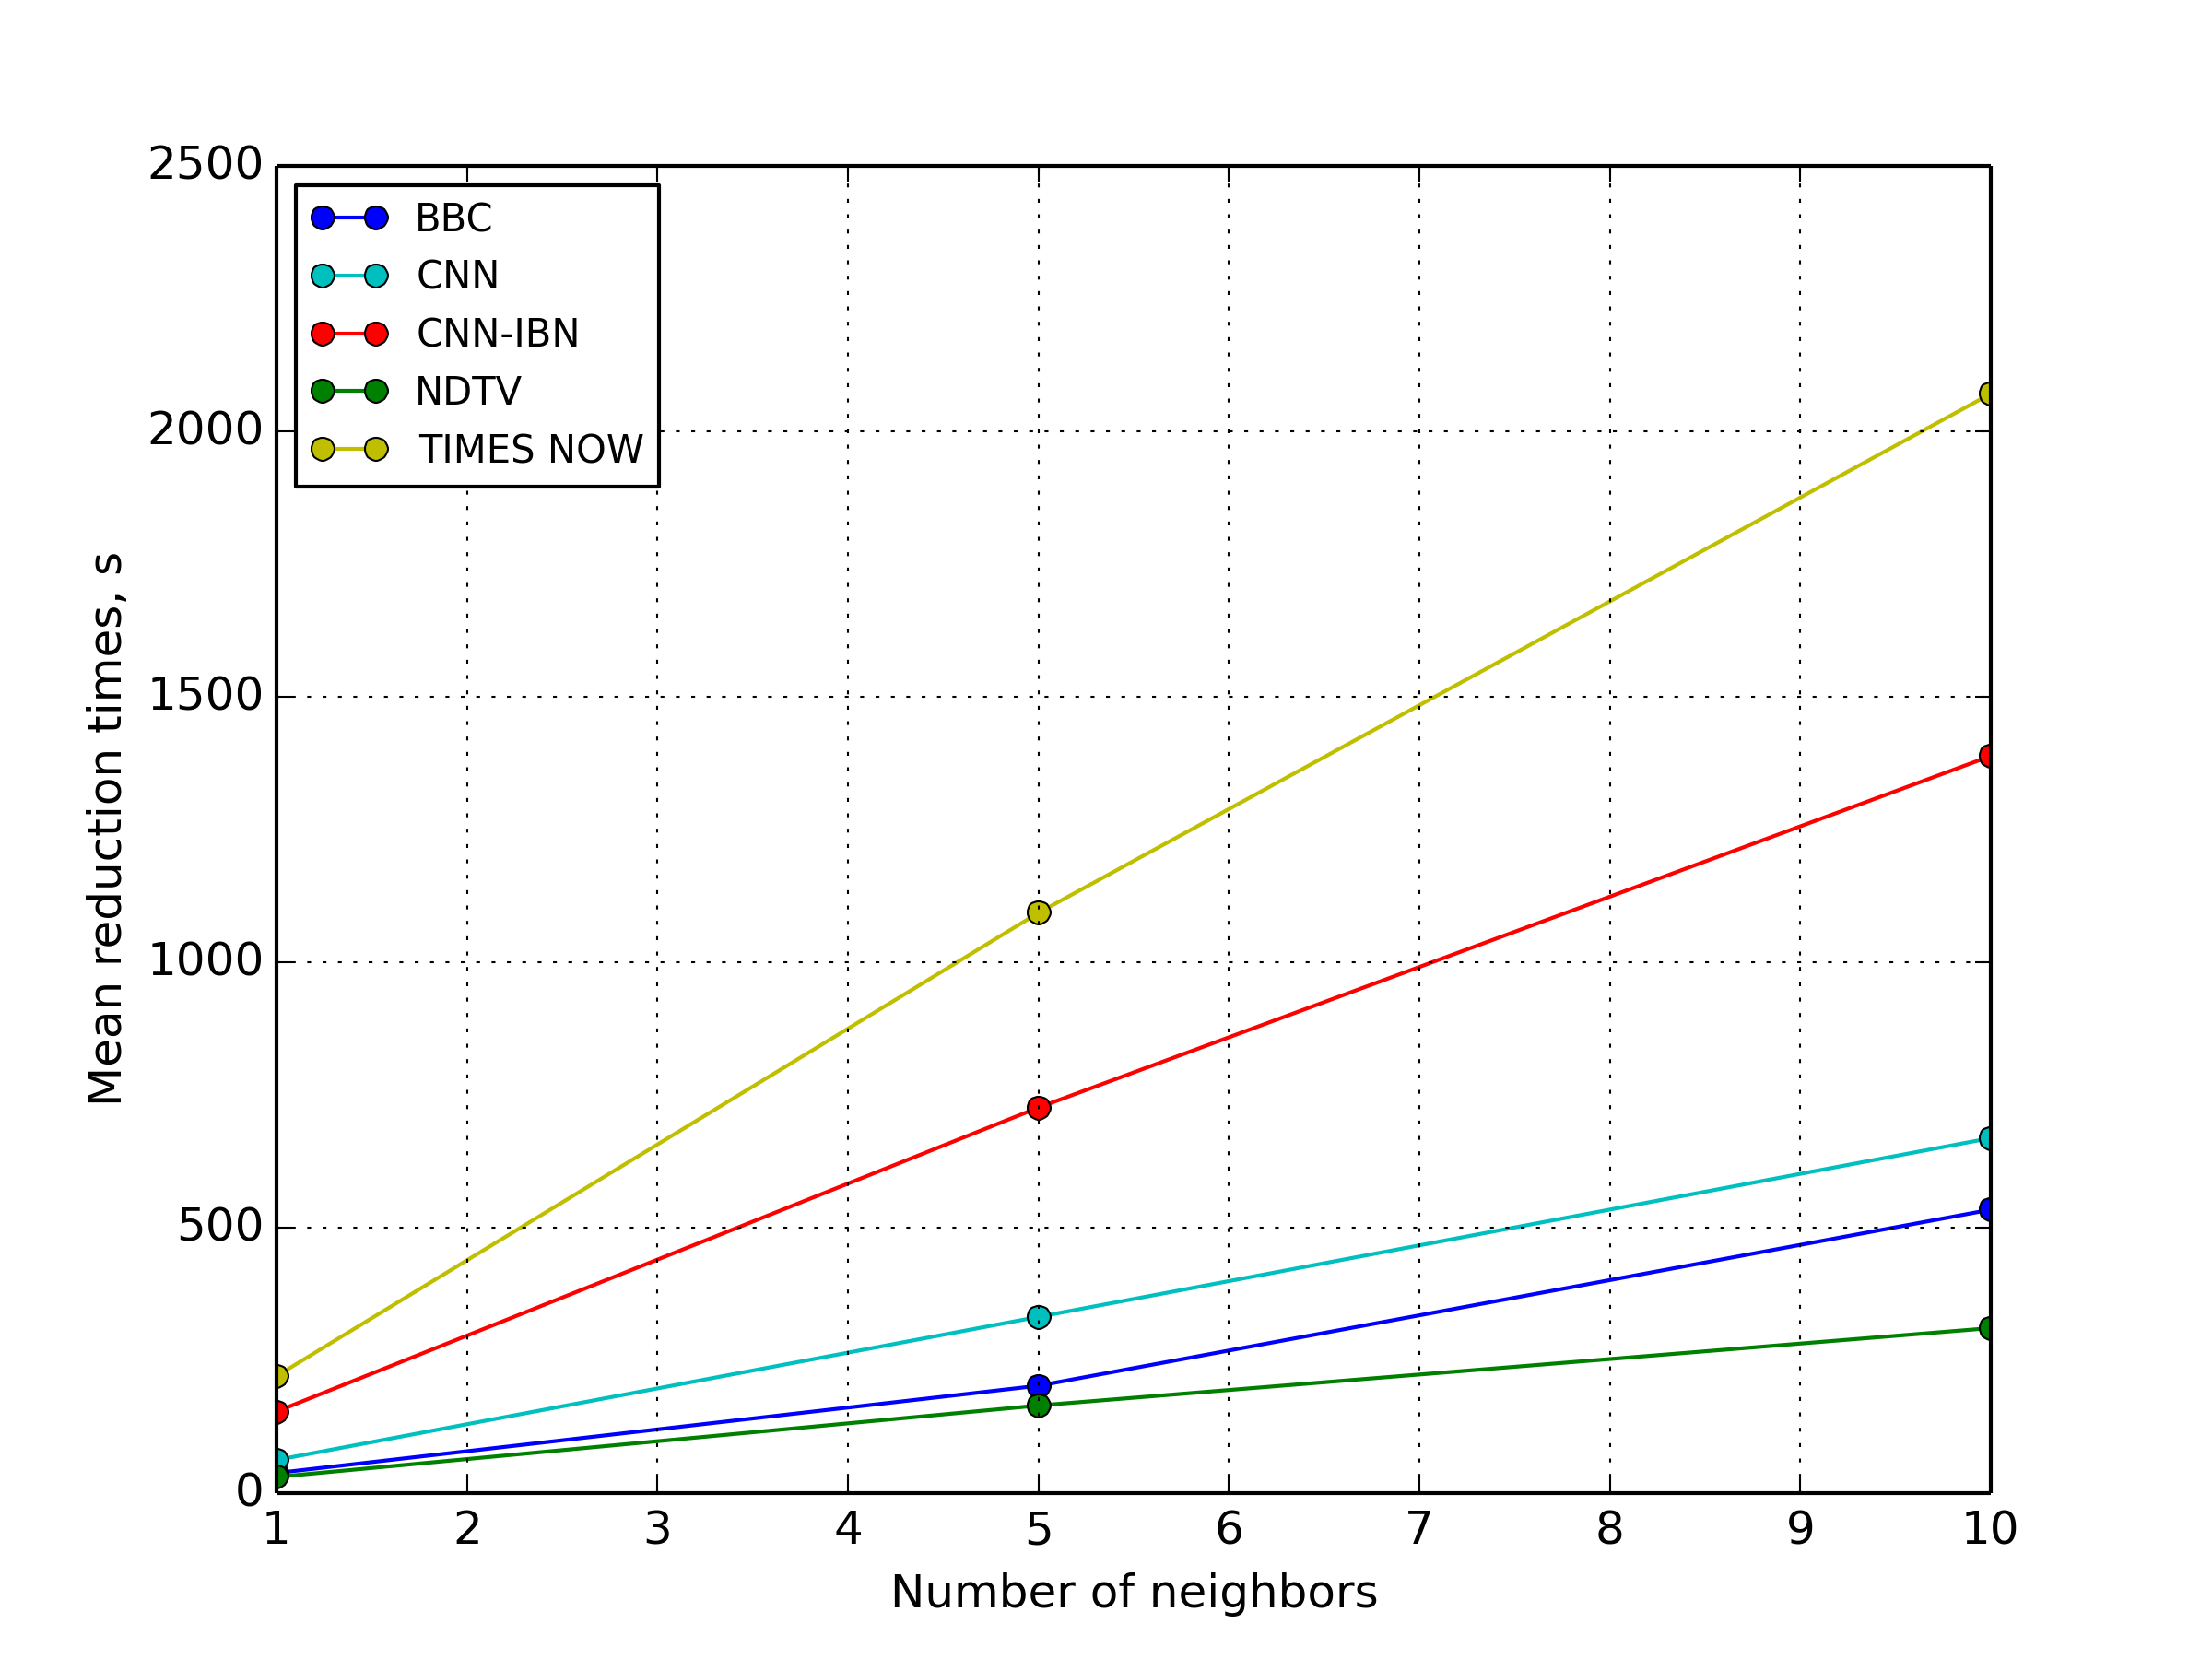
\includegraphics[width=\textwidth]{images/fcnn-TimeStats.png}
		\caption{Время, потраченное на отбор эталонов.}
	\end{subfigure}
	\caption{Результаты работы FCNN.}\label{fig:fcnn-stats}
\end{figure}

На рис.~\ref{fig:fcnn-knn-results}--\ref{fig:fcnn-gtb-results} приведены результаты работы базовых методах на обучающих выборках, редуцированных с помощью FCNN. \tbd{analysis}

\begin{figure}[h!]
    \centering
	\begin{subfigure}{0.45\textwidth}
		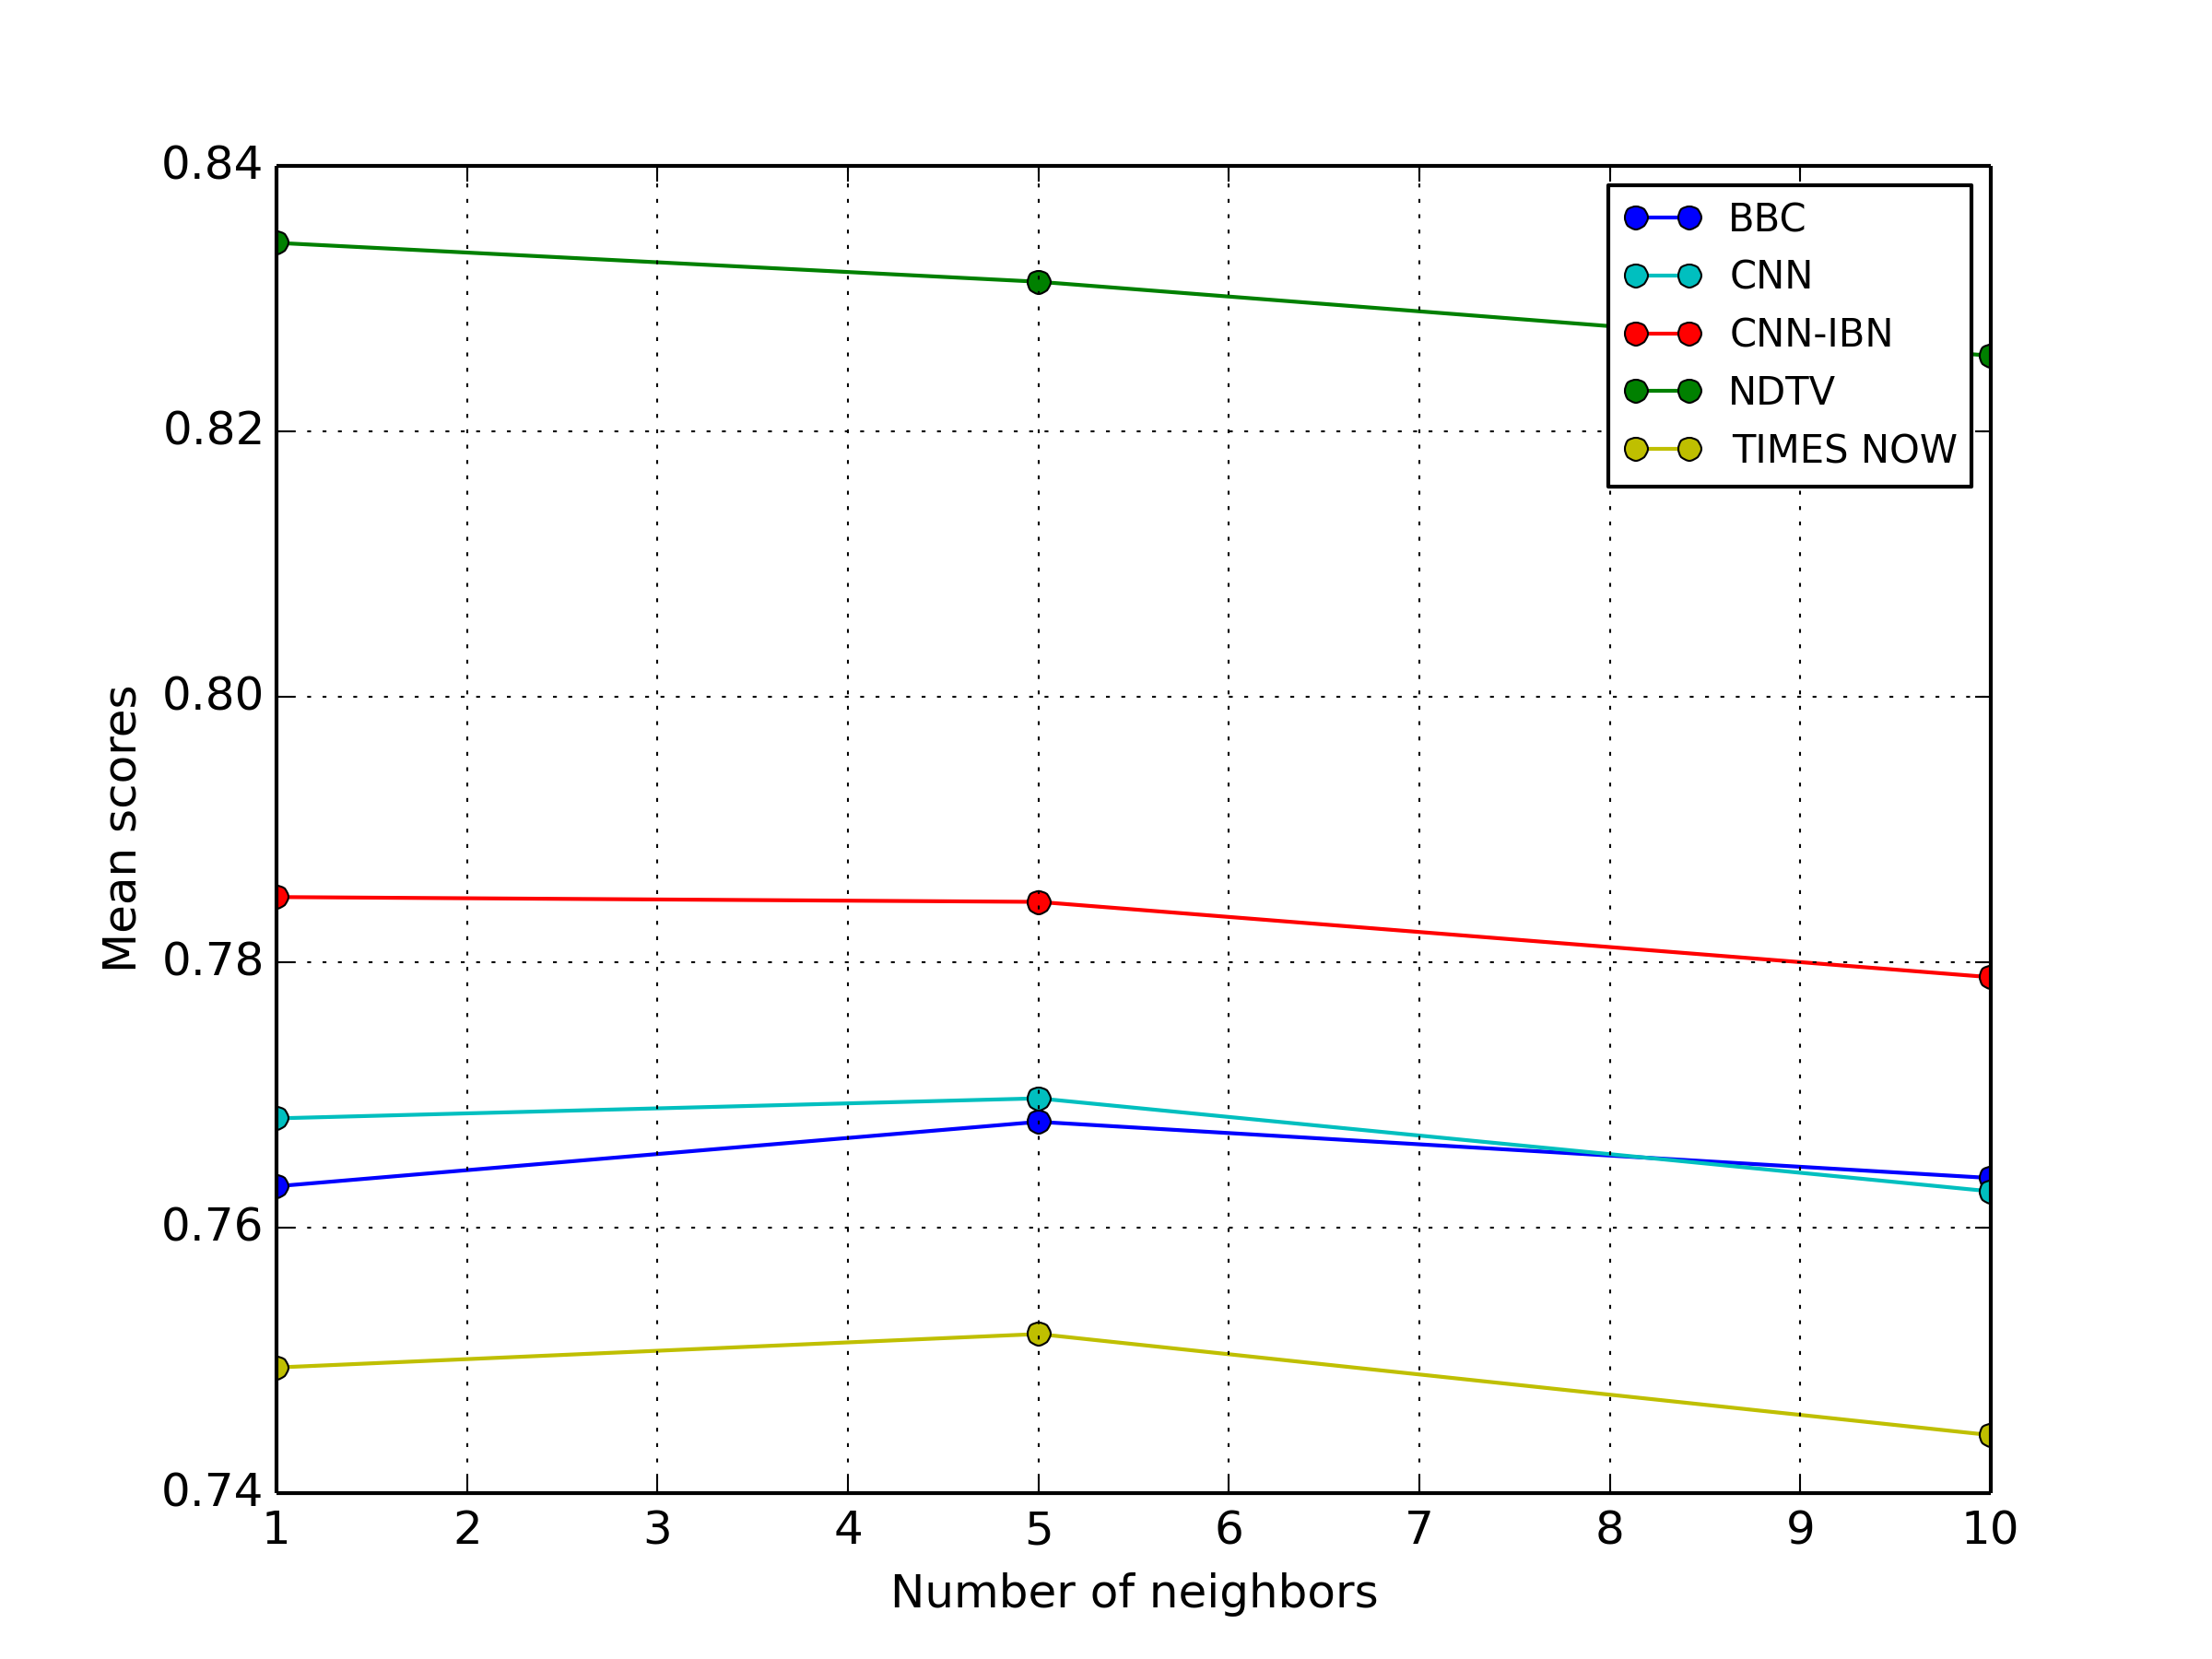
\includegraphics[width=\textwidth]{images/fcnn-KNN.png}
		\caption{Качество классификации.}
	\end{subfigure}
	\begin{subfigure}{0.45\textwidth}
		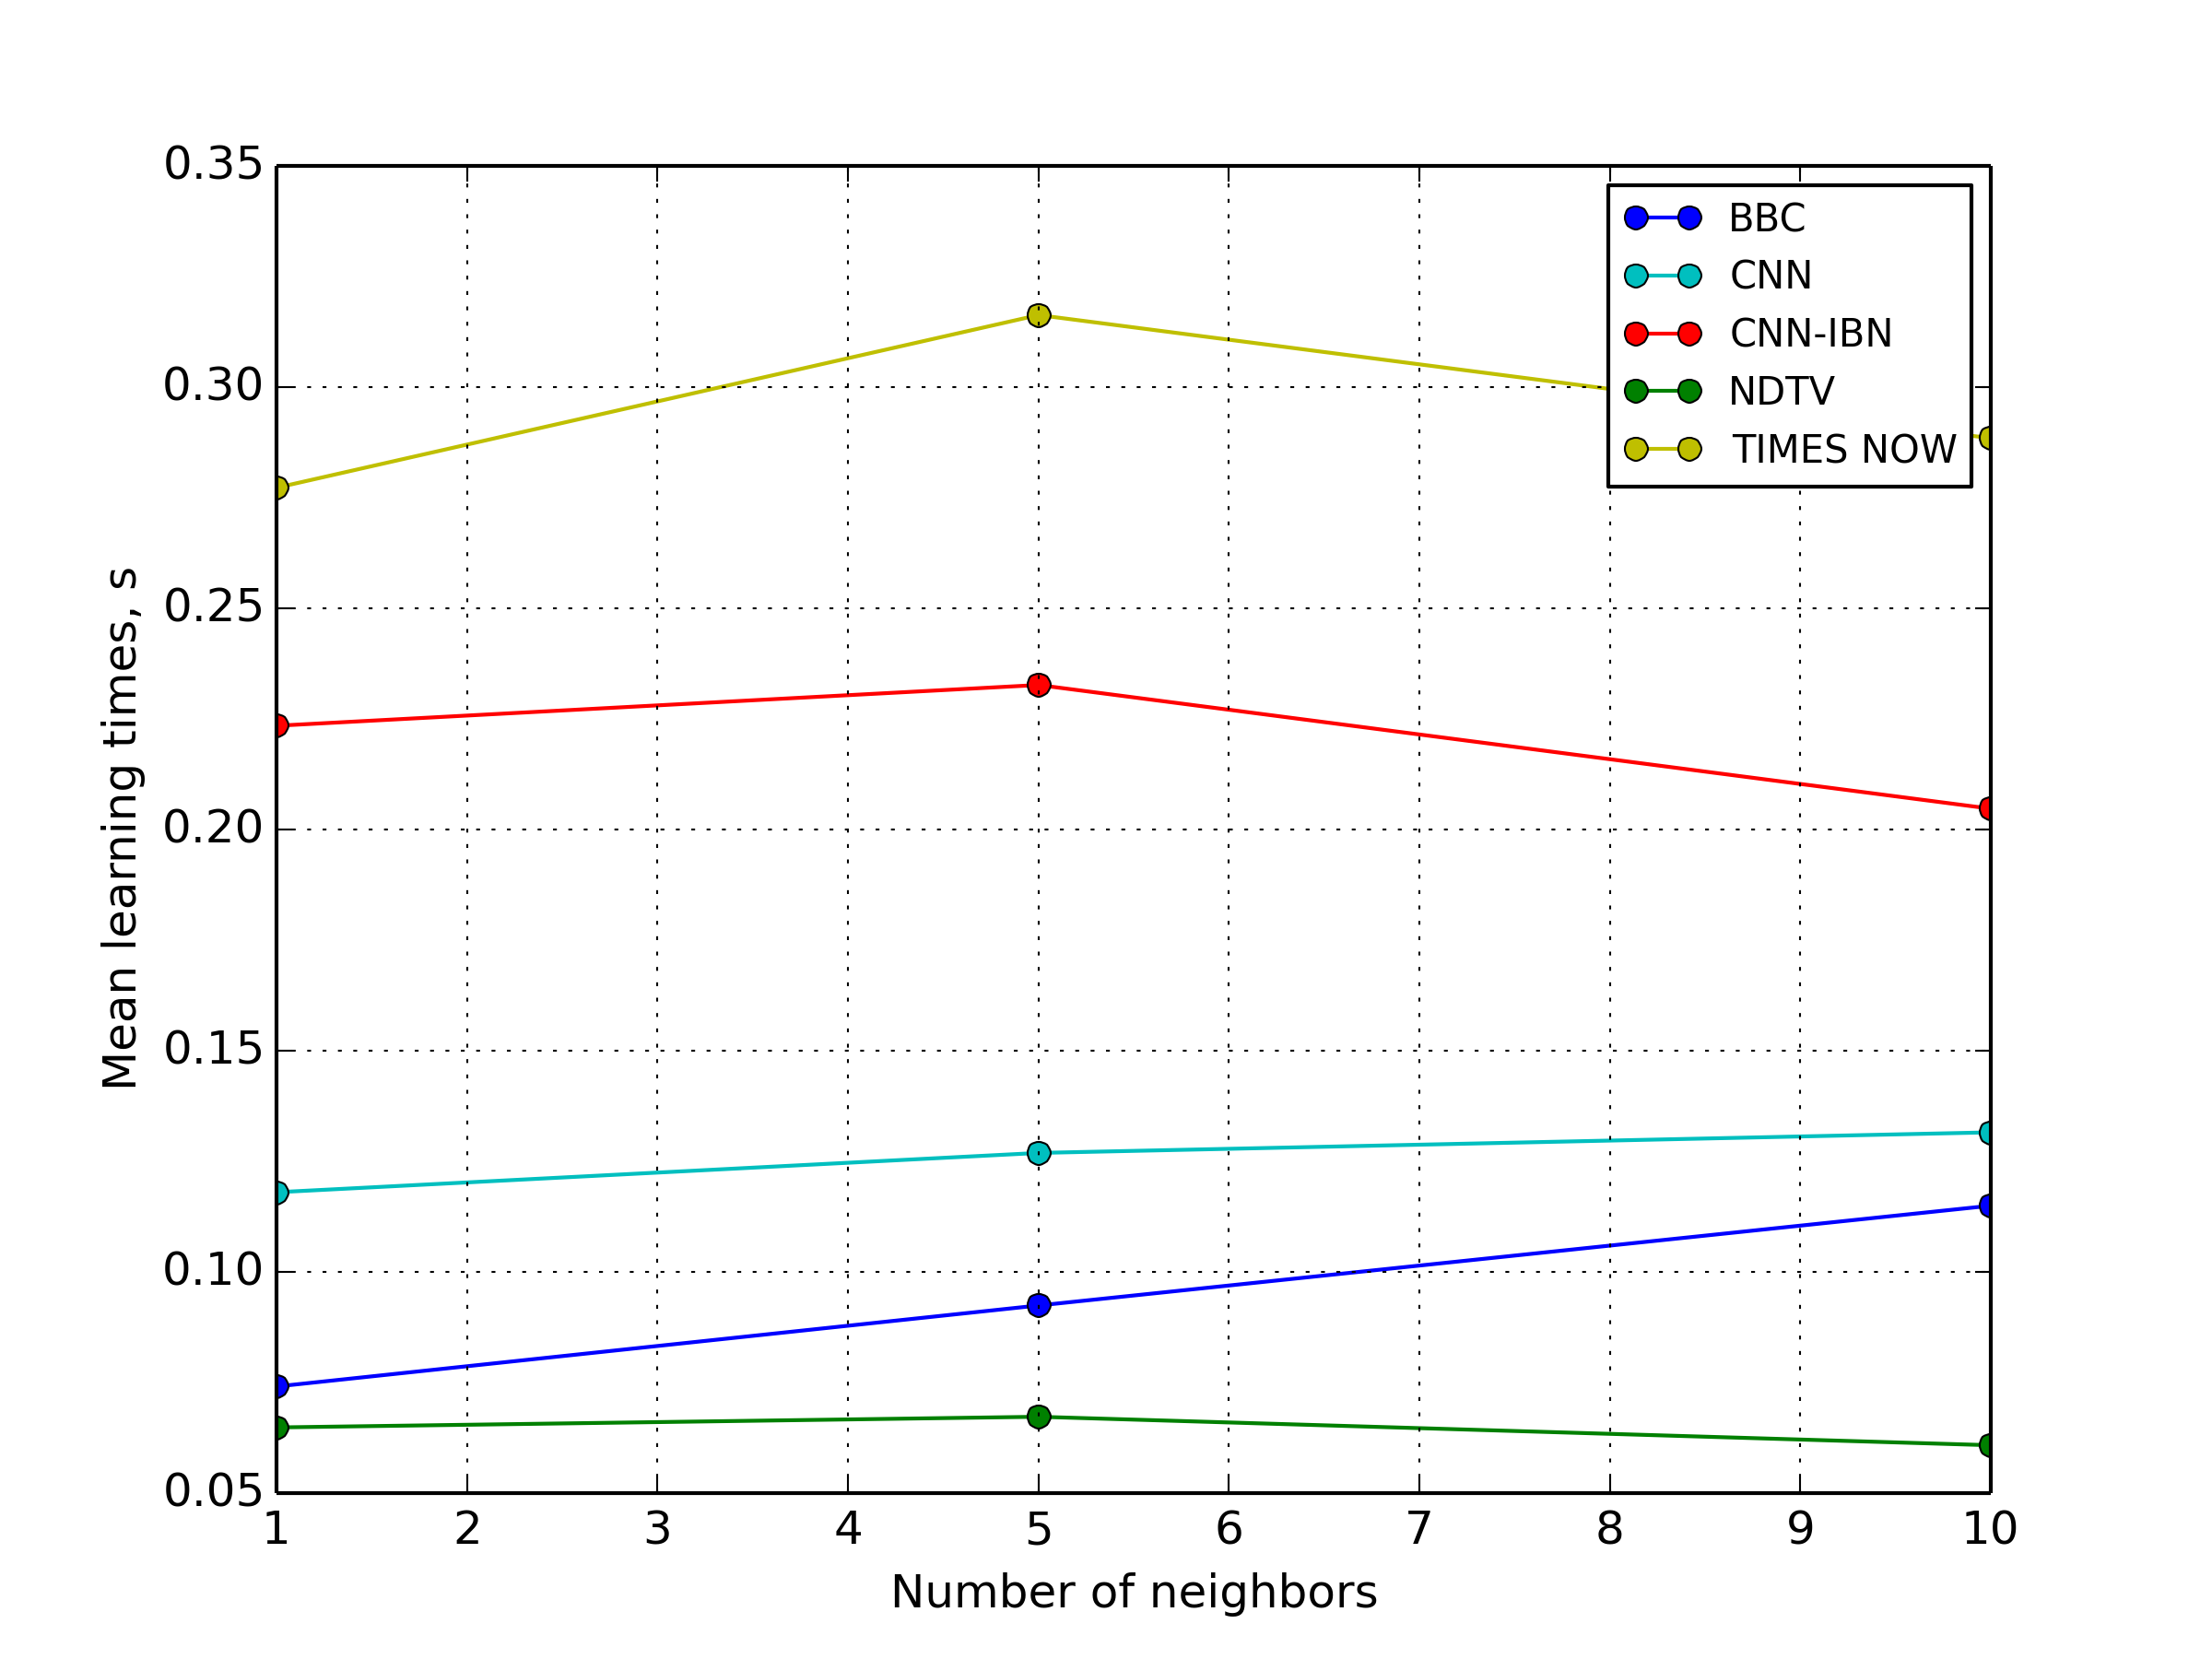
\includegraphics[width=\textwidth]{images/fcnn-KNNTime.png}
		\caption{Время обучения.}
	\end{subfigure}
	\caption{Результаты применения FCNN для 15-NN.}\label{fig:fcnn-knn-results}
\end{figure}

\begin{figure}[h!]
	\centering
	\begin{subfigure}{0.45\textwidth}
		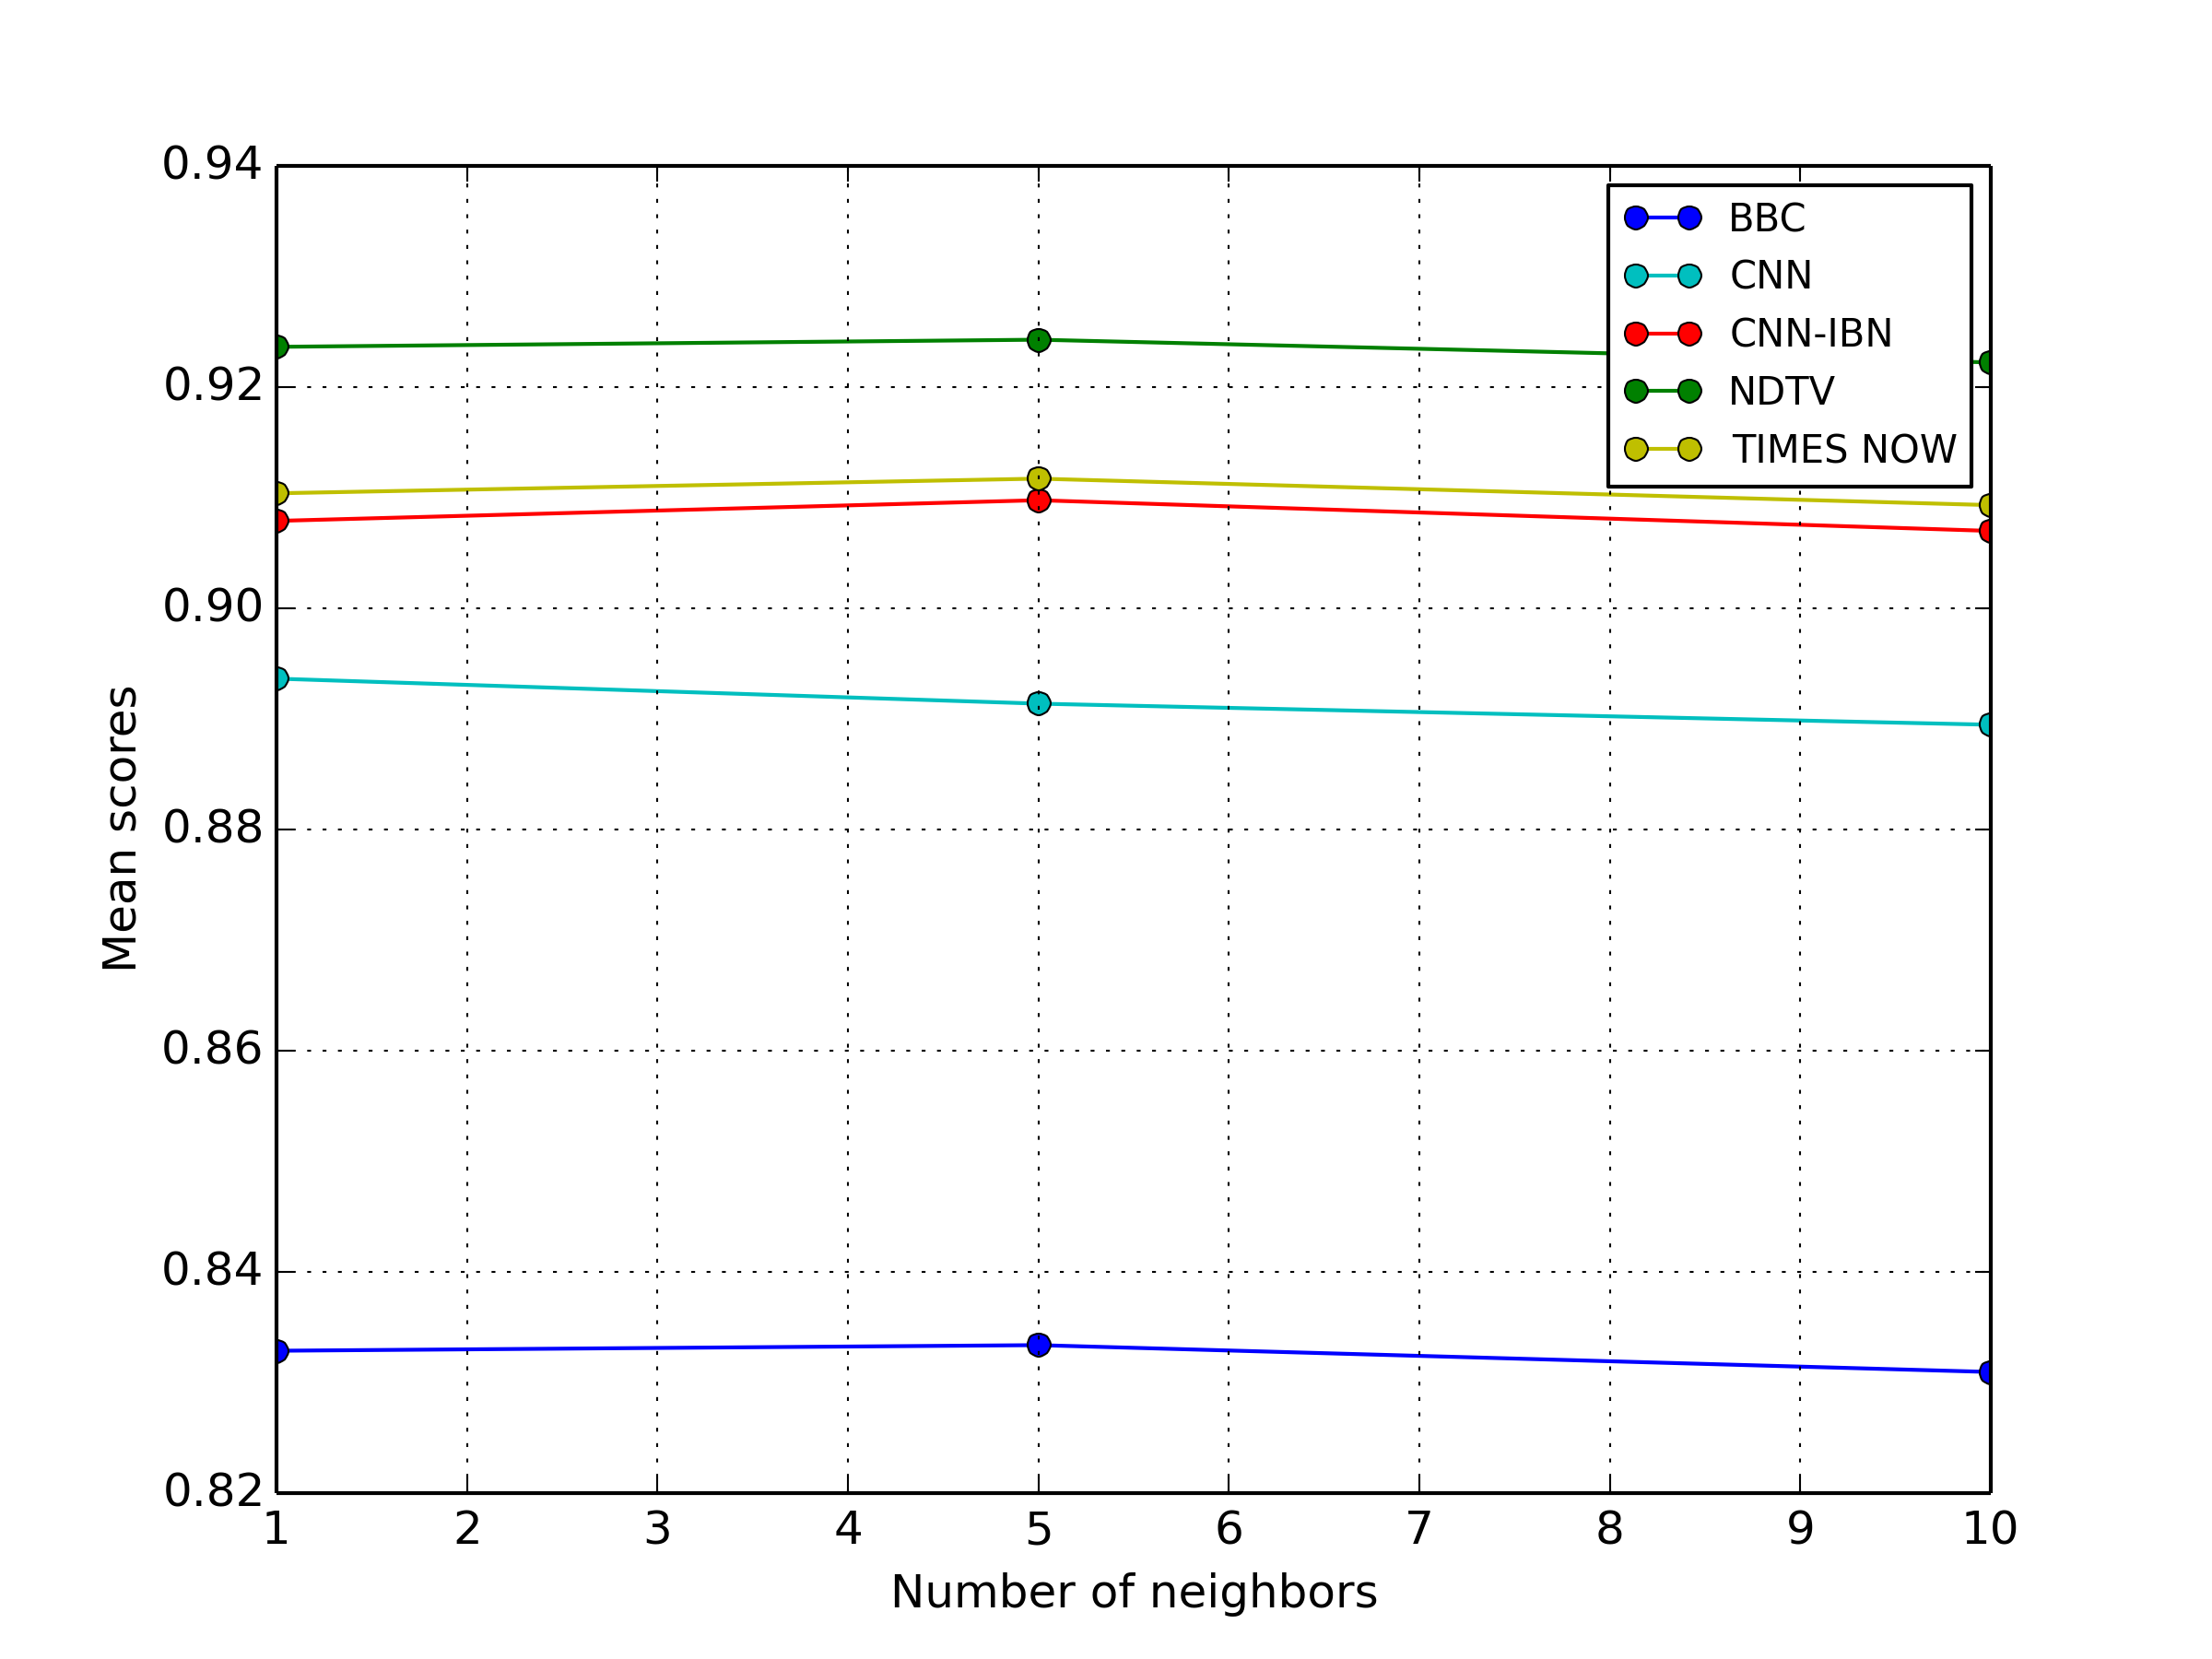
\includegraphics[width=\textwidth]{images/fcnn-LDA.png}
		\caption{Качество классификации.}
	\end{subfigure}
	\begin{subfigure}{0.45\textwidth}
		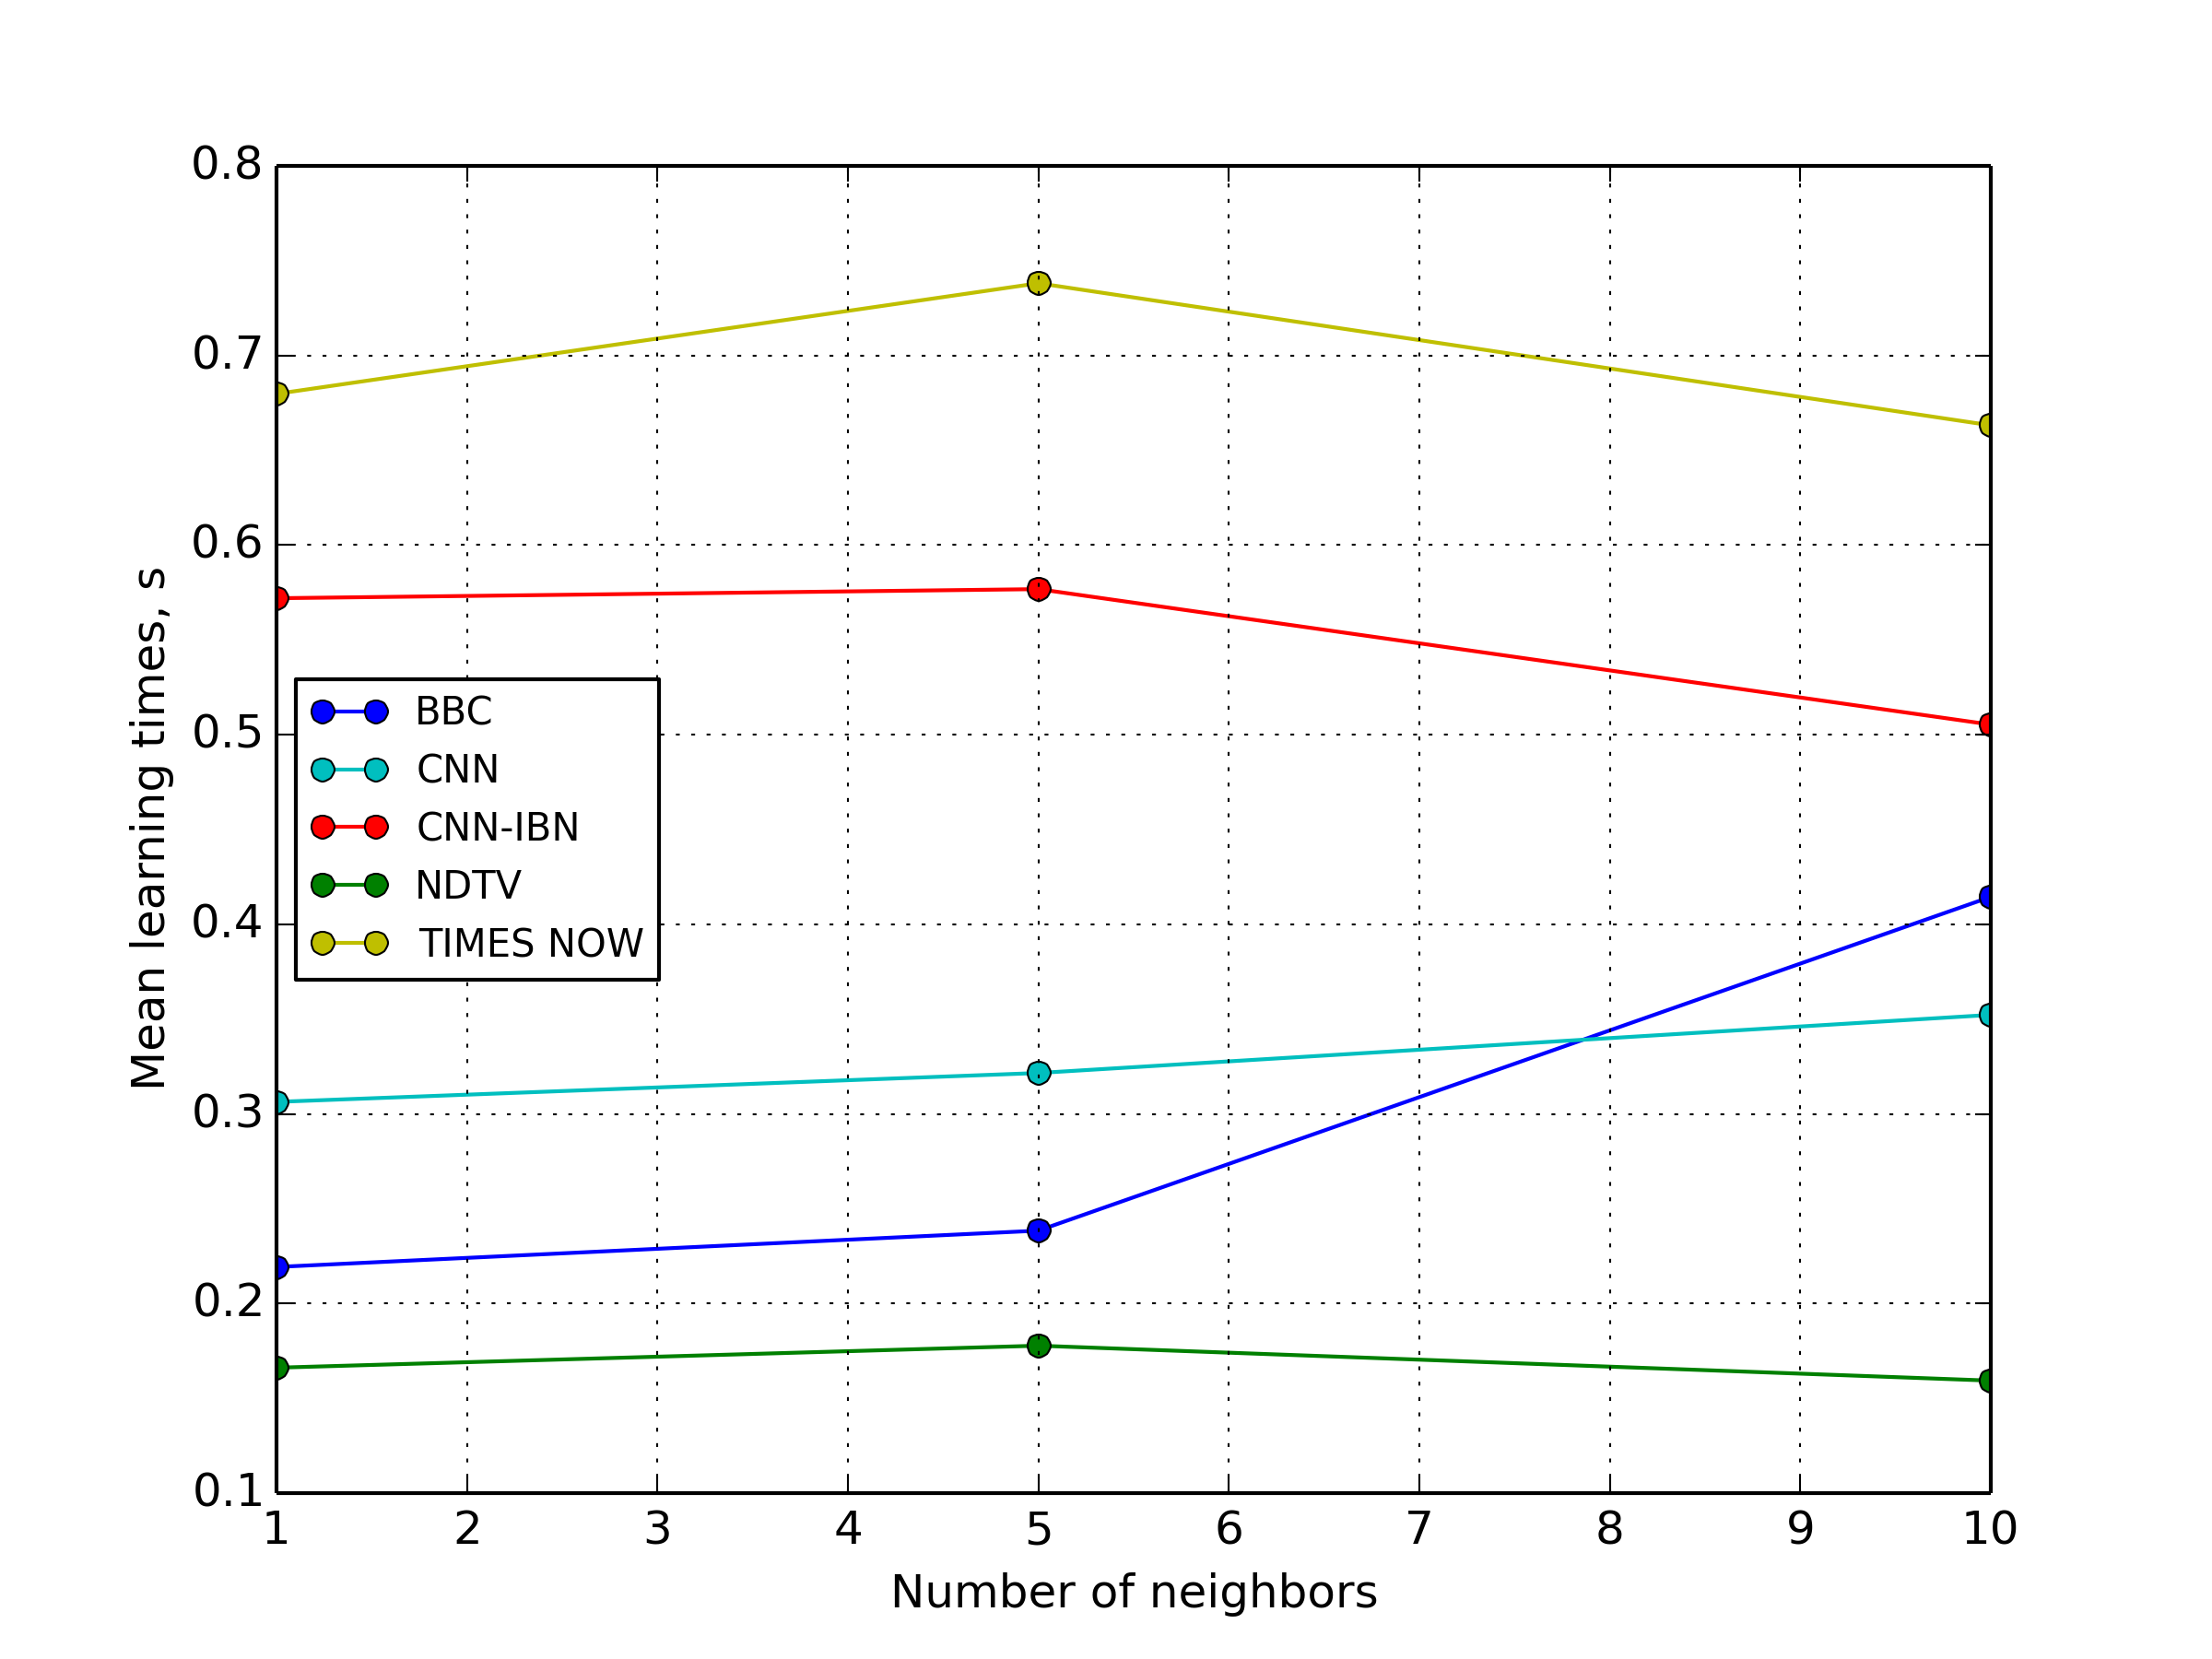
\includegraphics[width=\textwidth]{images/fcnn-LDATime.png}
		\caption{Время обучения.}
	\end{subfigure}
	\caption{Результаты применения FCNN для LDA.}\label{fig:fcnn-lda-results}
\end{figure}

\begin{figure}[h!]
	\centering
	\begin{subfigure}{0.45\textwidth}
		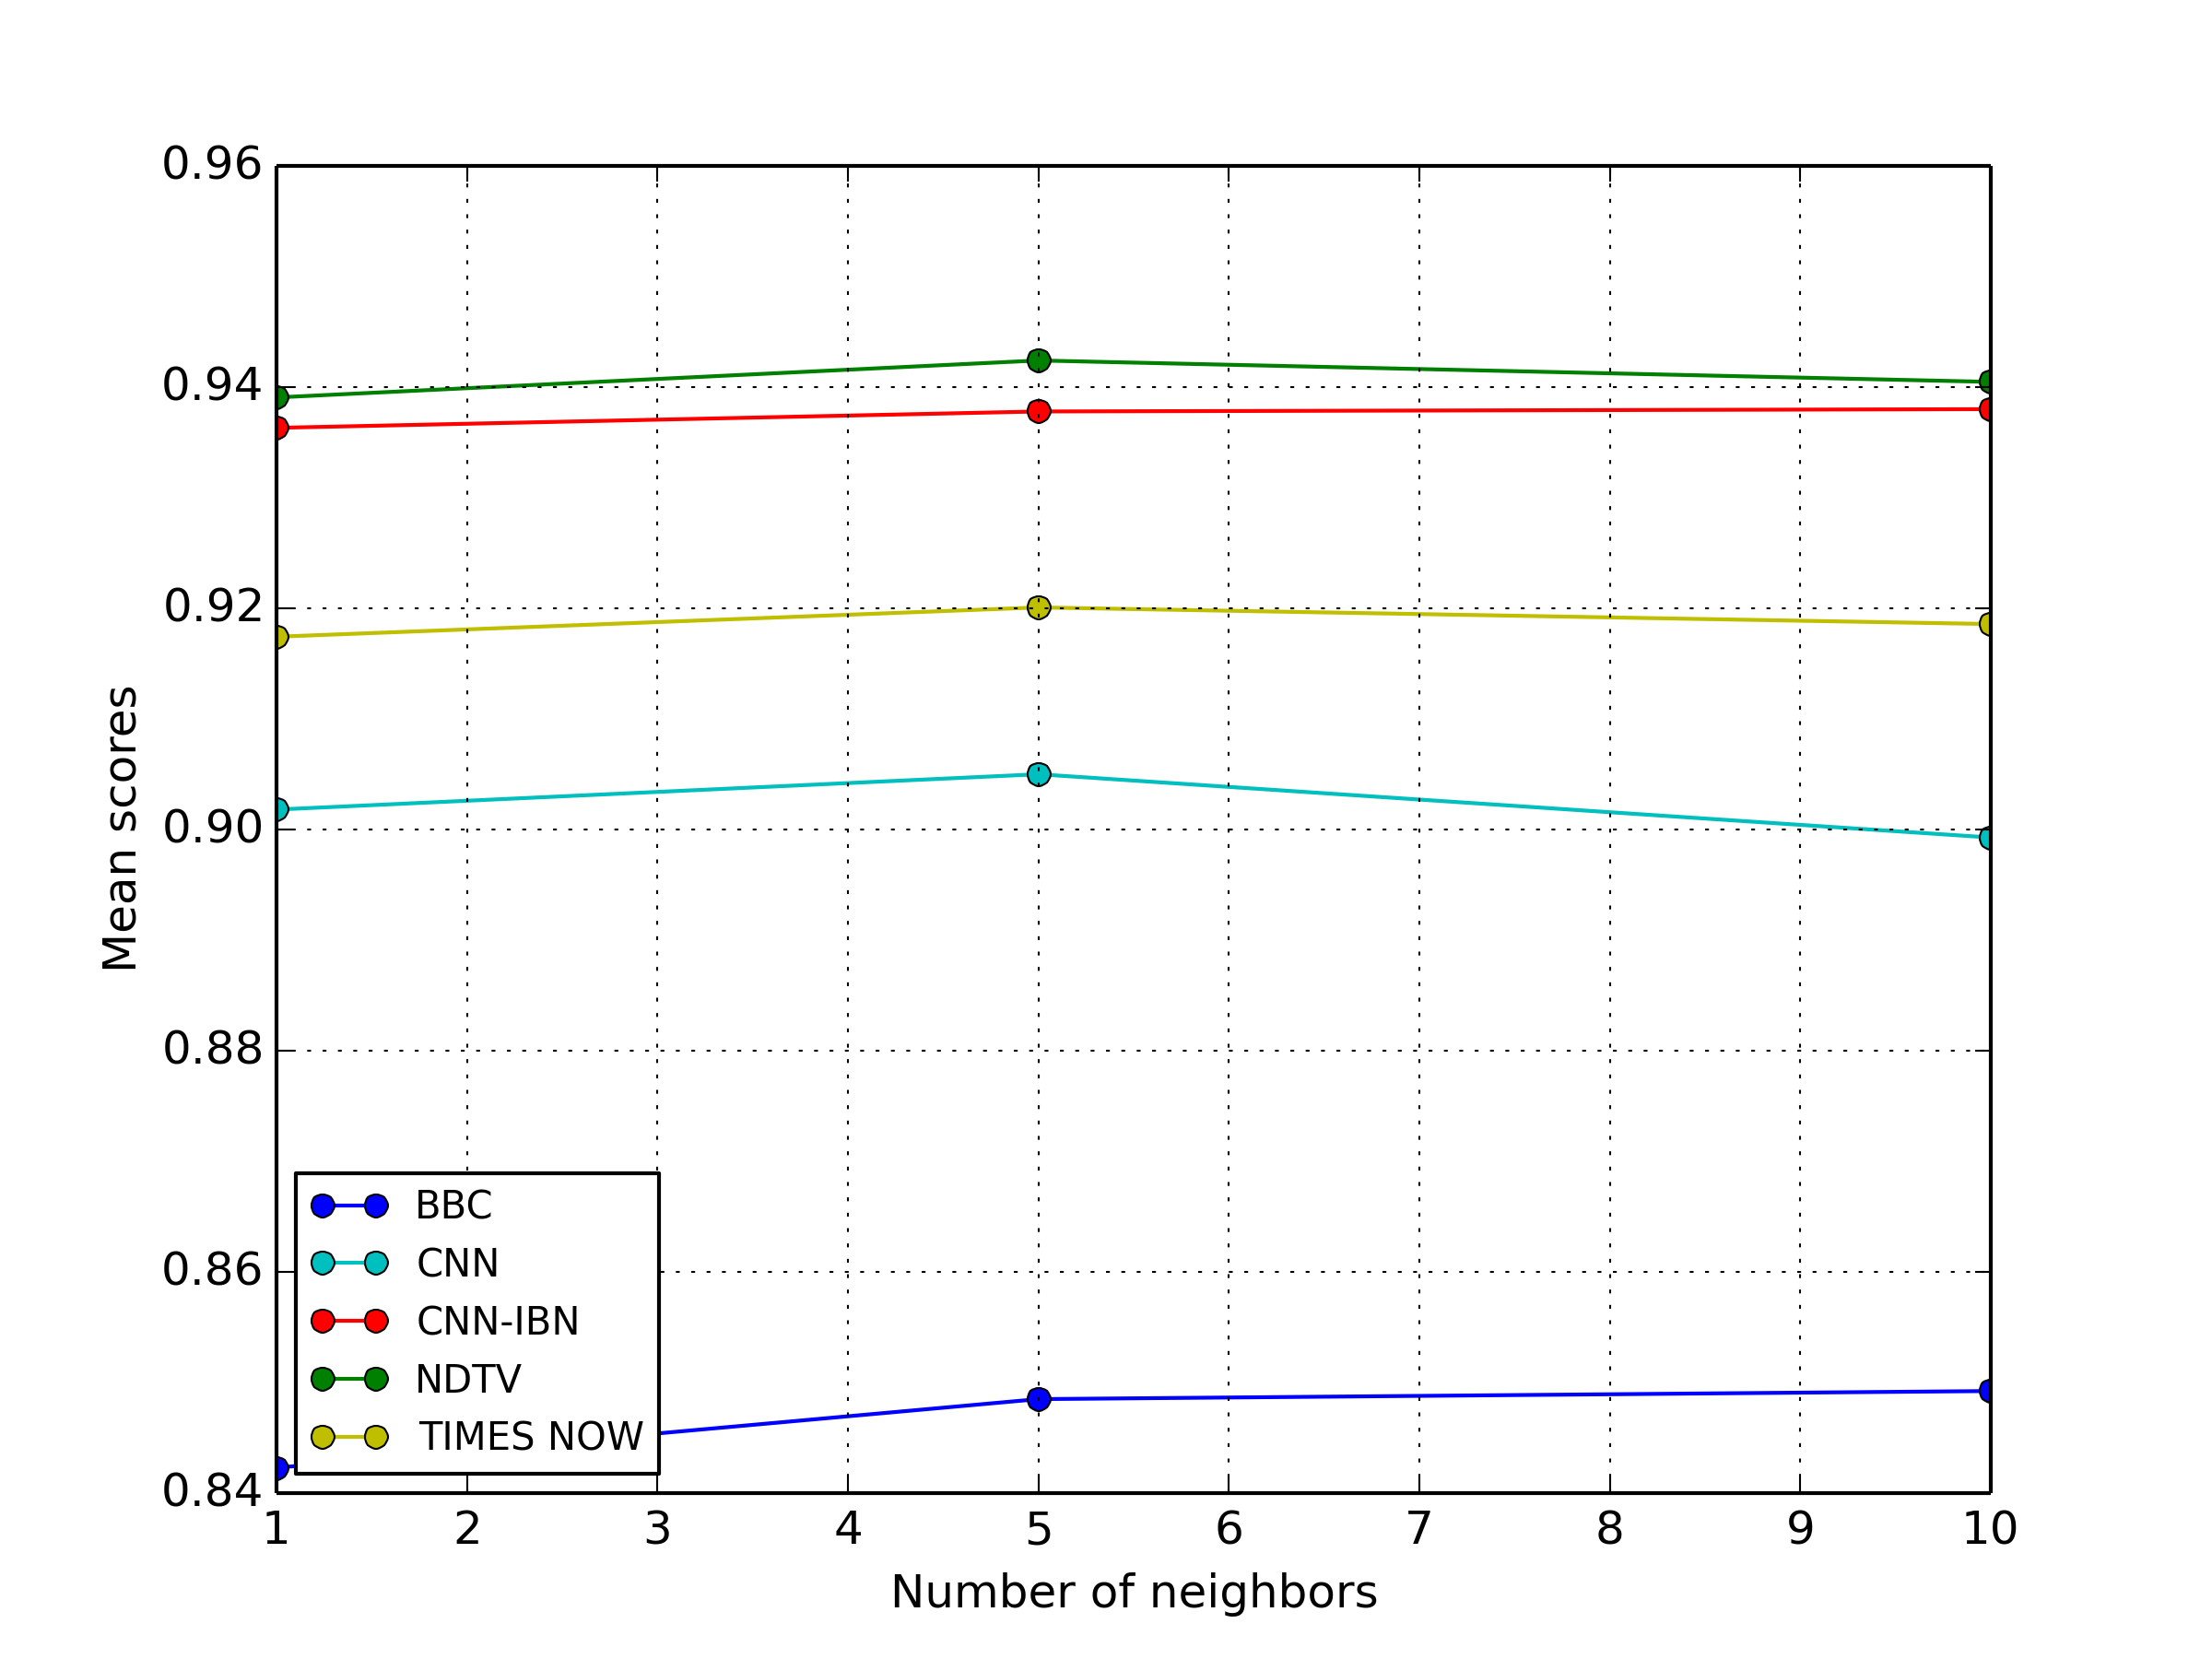
\includegraphics[width=\textwidth]{images/fcnn-SVM.png}
		\caption{Качество классификации.}
	\end{subfigure}
	\begin{subfigure}{0.45\textwidth}
		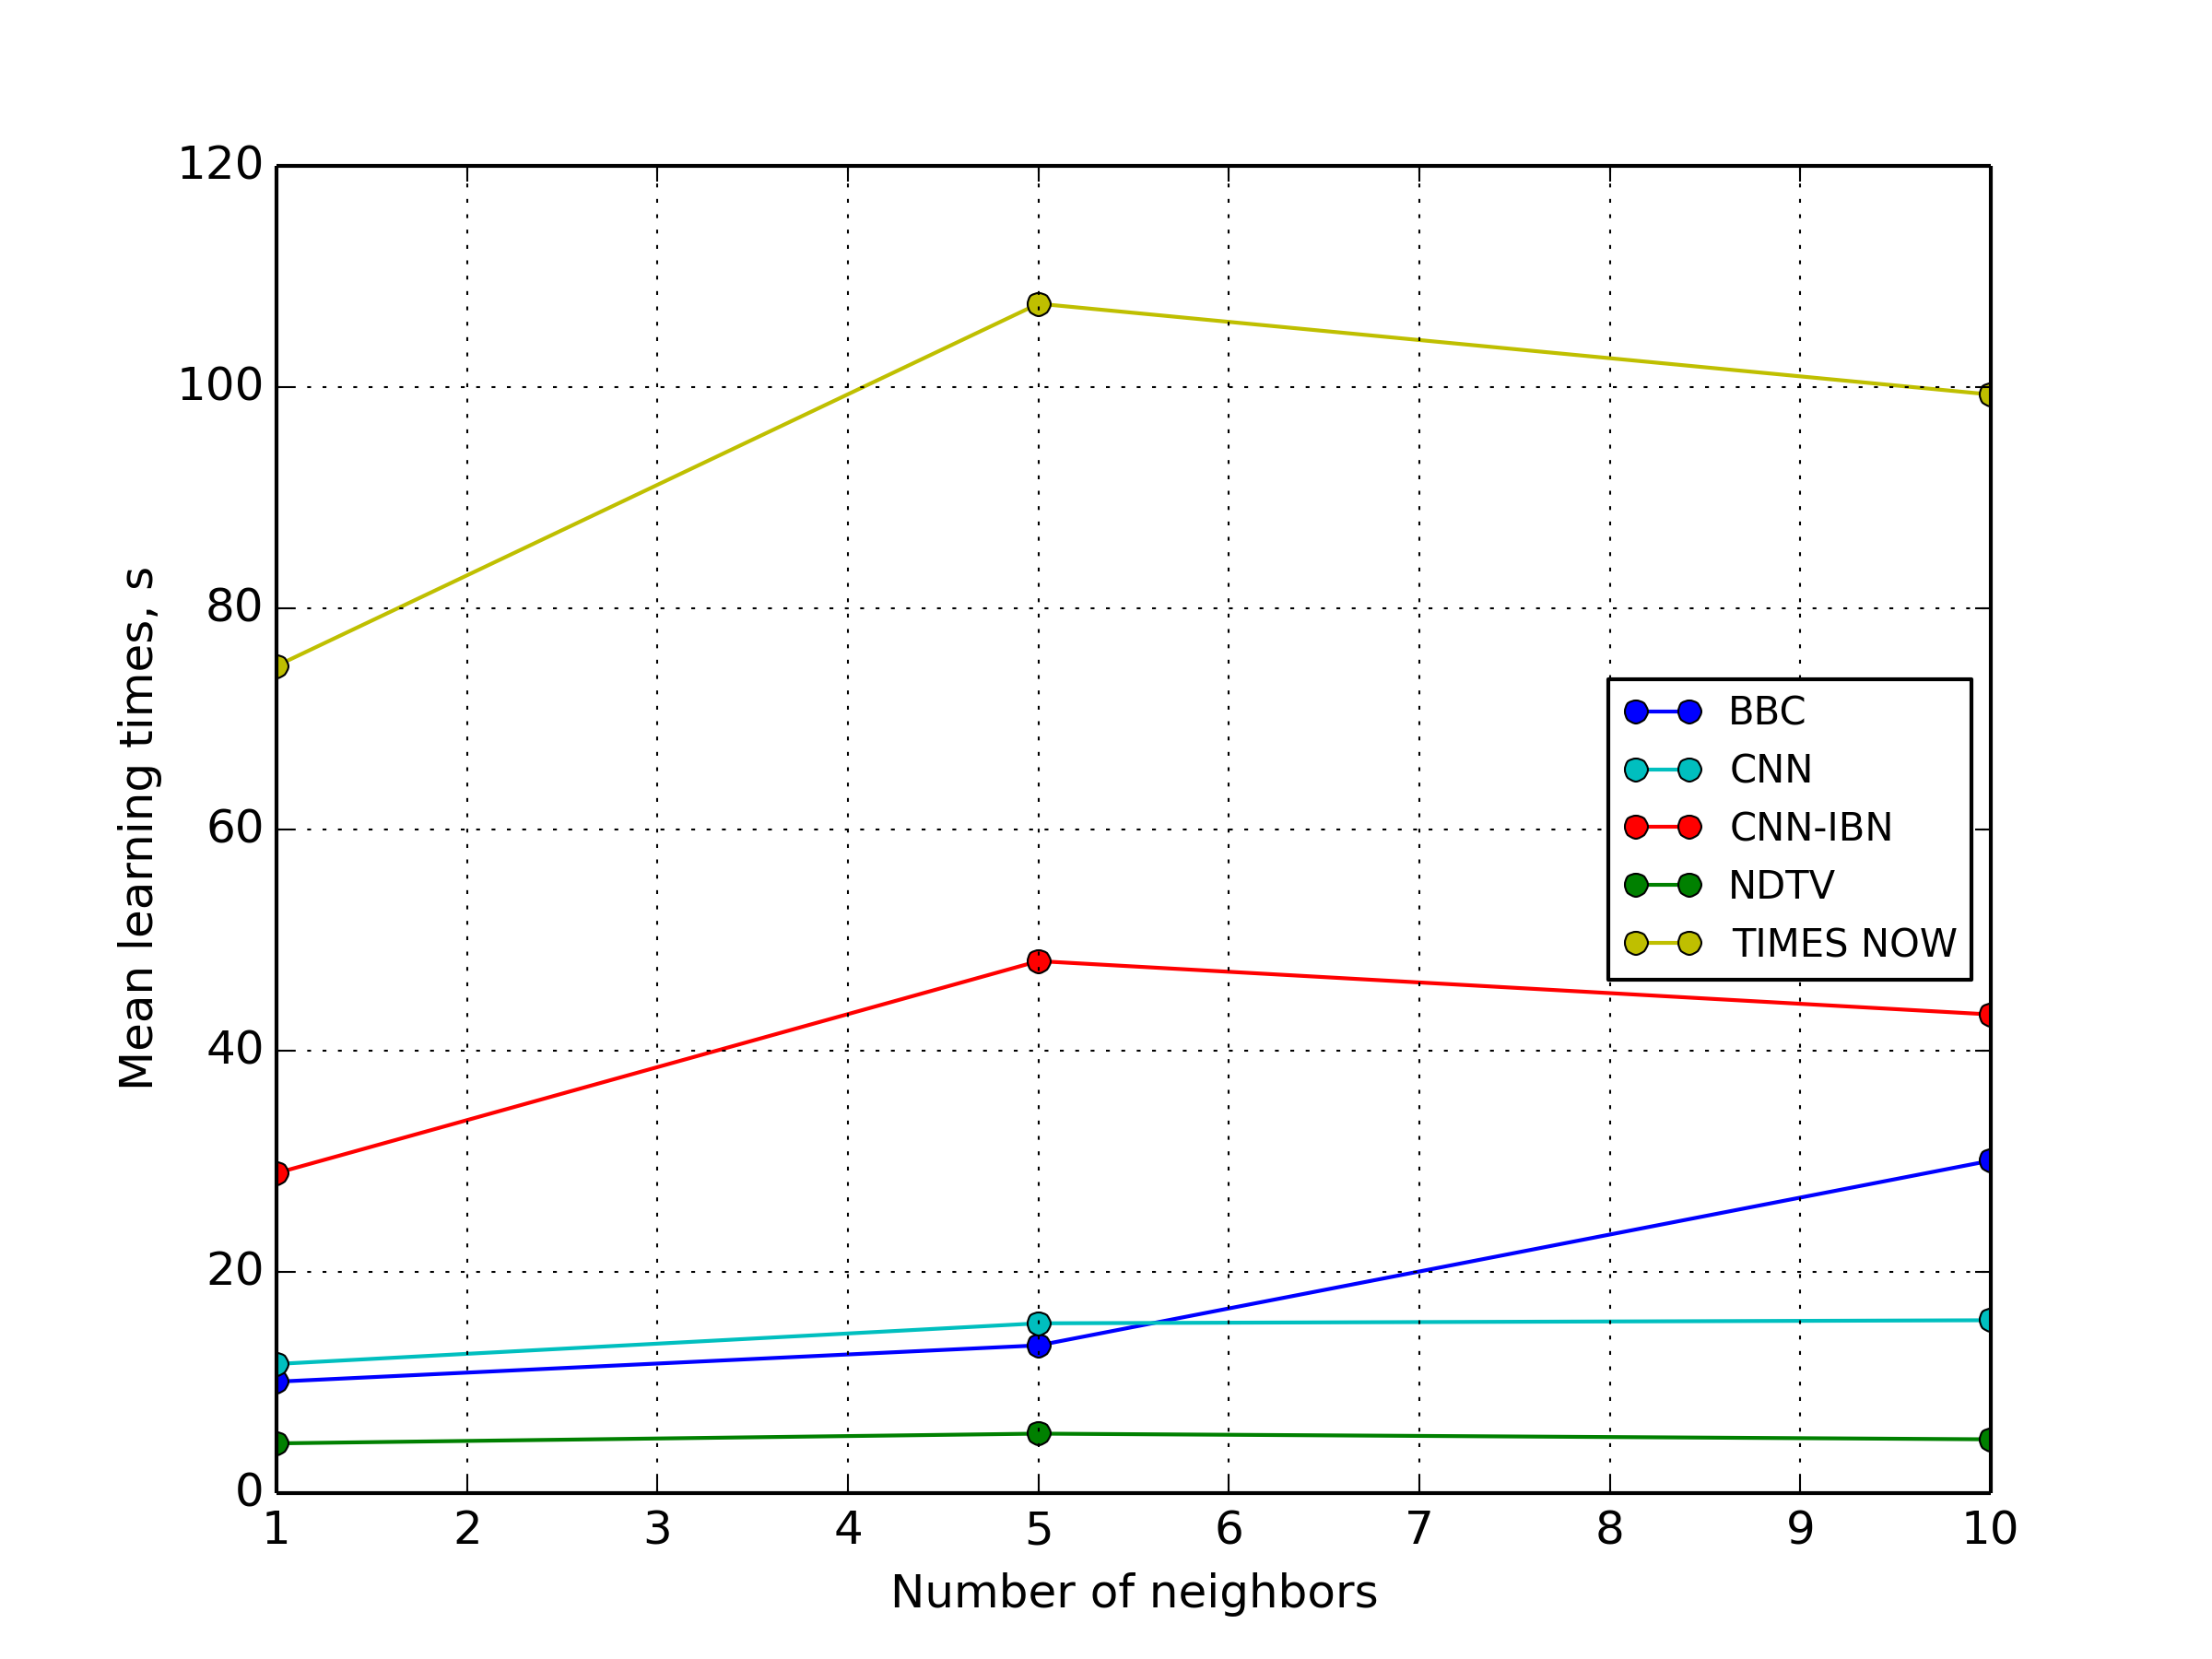
\includegraphics[width=\textwidth]{images/fcnn-SVMTime.png}
		\caption{Время обучения.}
	\end{subfigure}
	\caption{Результаты применения FCNN для SVM.}\label{fig:fcnn-svm-results}
\end{figure}

\begin{figure}[h!]
	\centering
	\begin{subfigure}{0.45\textwidth}
		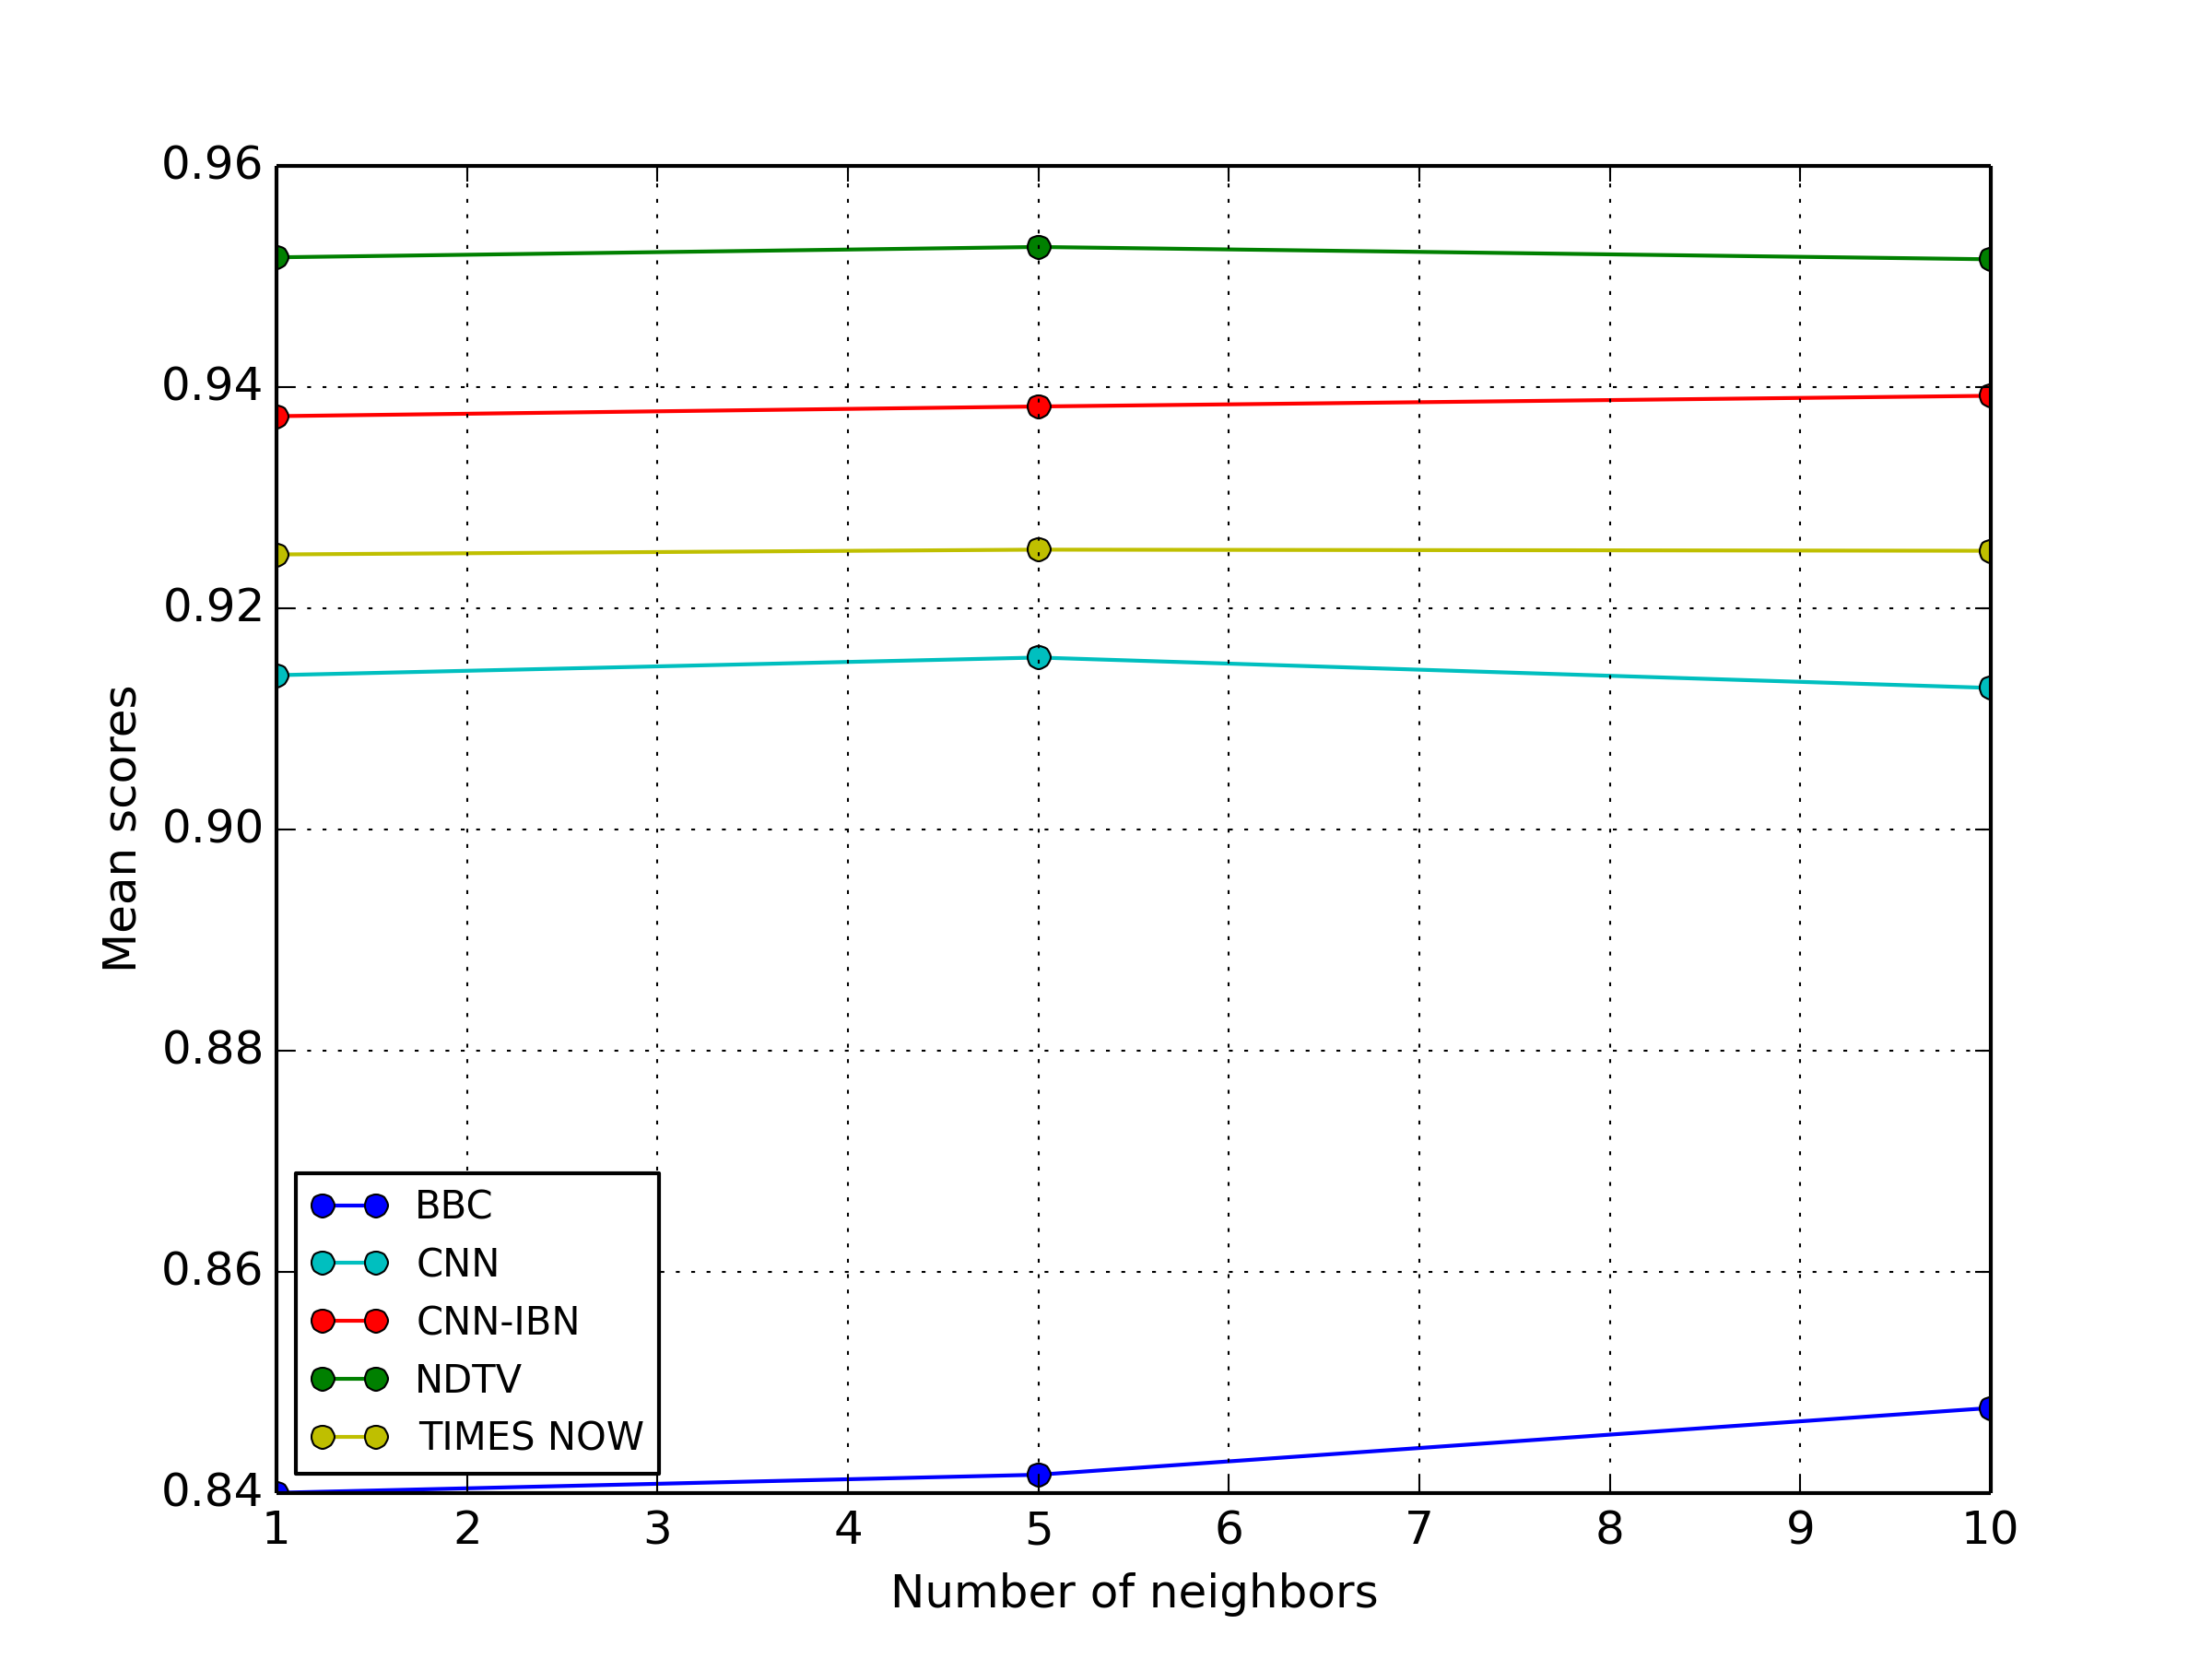
\includegraphics[width=\textwidth]{images/fcnn-randforest.png}
		\caption{Качество классификации.}
	\end{subfigure}
	\begin{subfigure}{0.45\textwidth}
		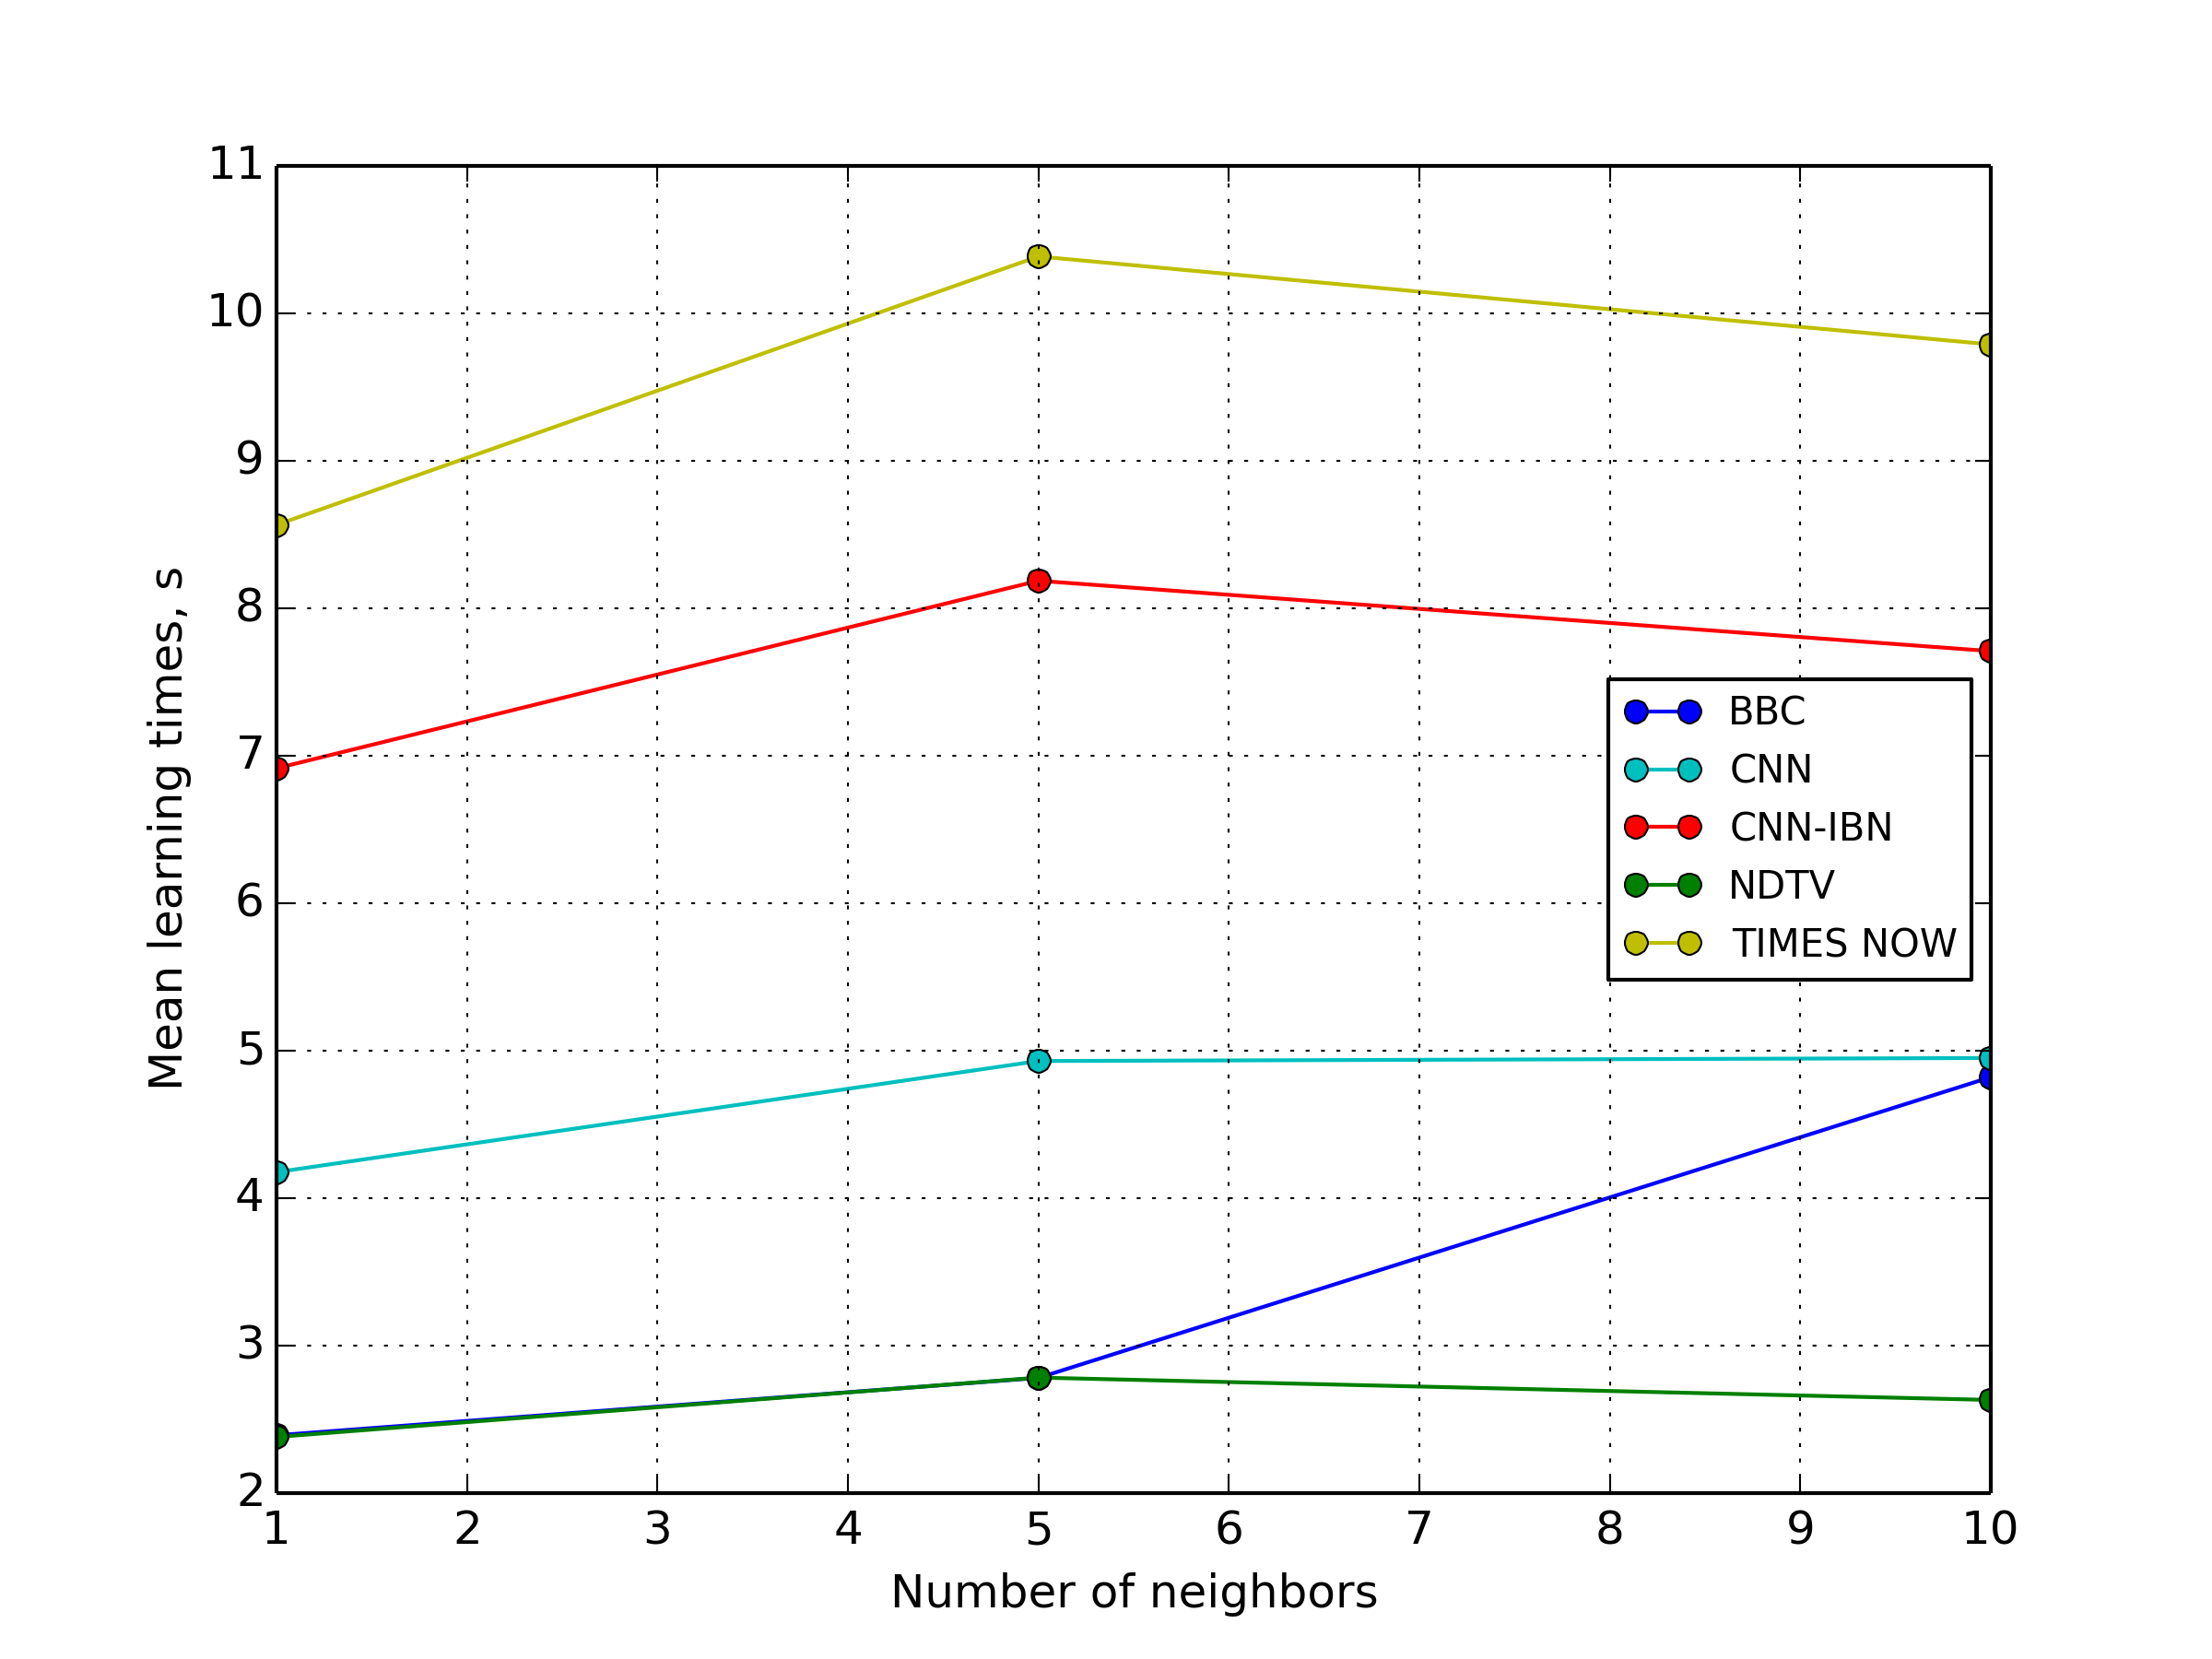
\includegraphics[width=\textwidth]{images/fcnn-randforestTime.png}
		\caption{Время обучения.}
	\end{subfigure}
	\caption{Результаты применения FCNN для Random forest.}\label{fig:fcnn-rf-results}
\end{figure}

\begin{figure}
	\centering
	\begin{subfigure}{0.45\textwidth}
		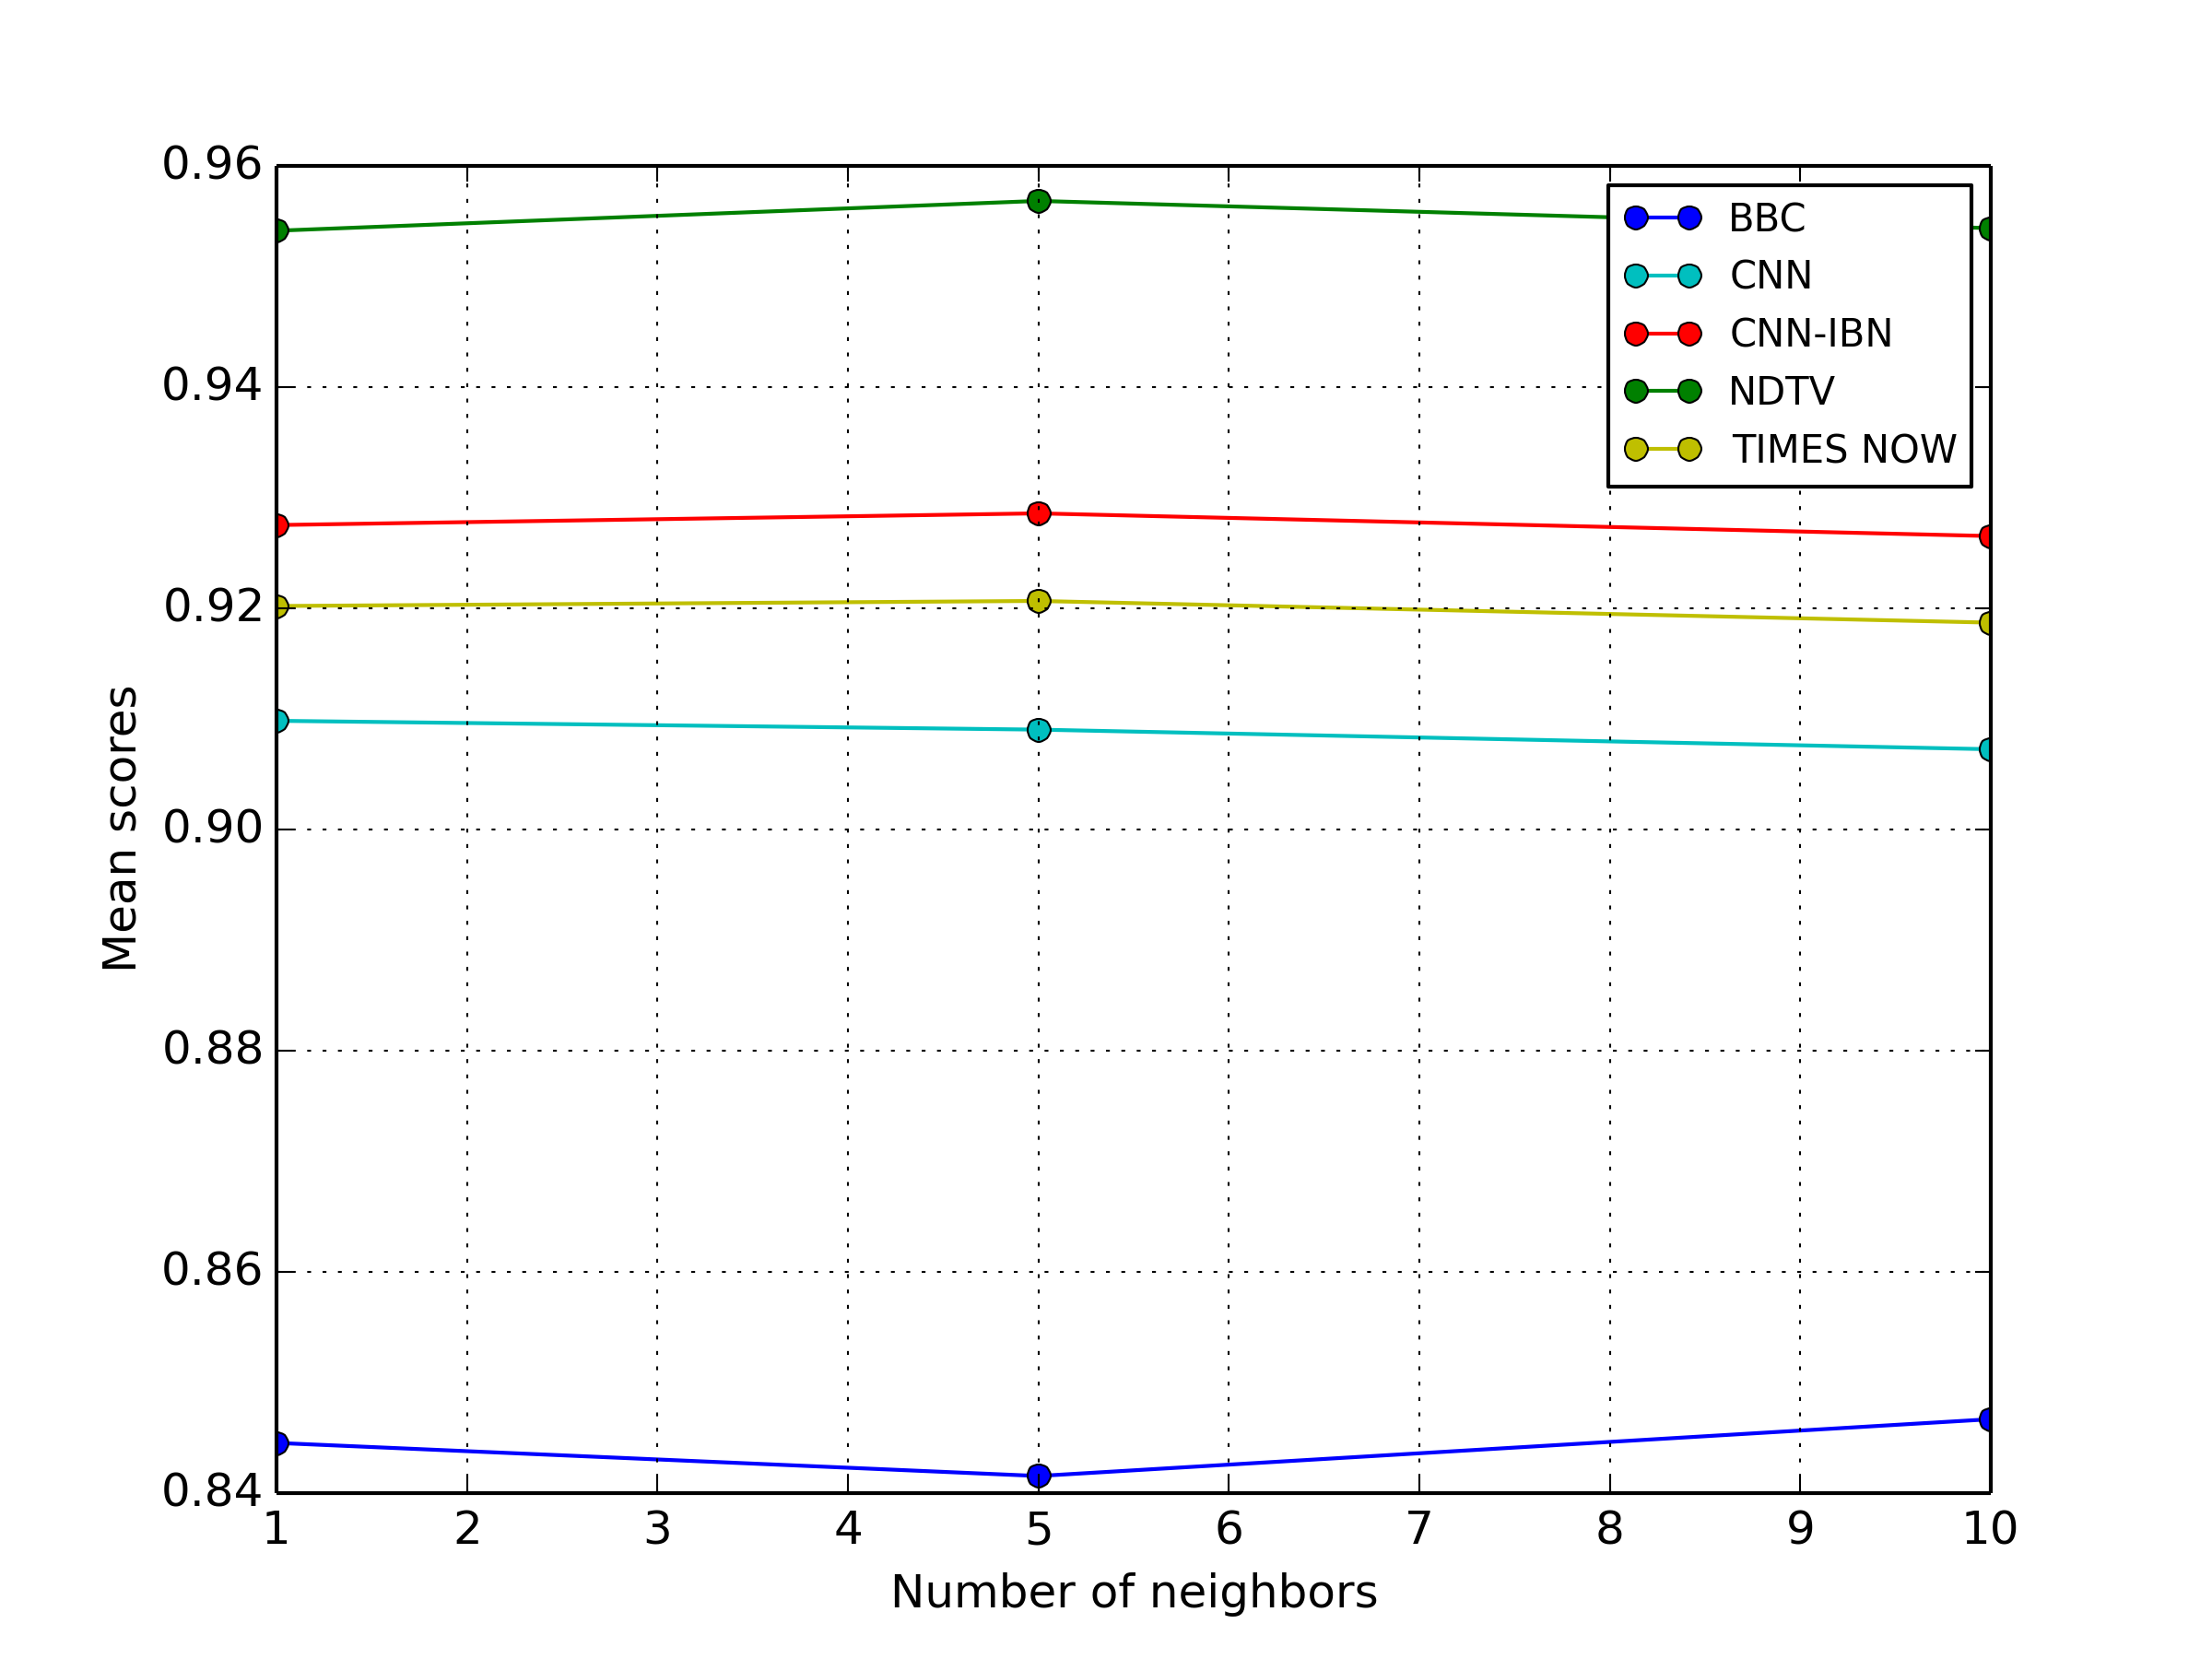
\includegraphics[width=\textwidth]{images/fcnn-gradboosting.png}
		\caption{Качество классификации.}
	\end{subfigure}
	\begin{subfigure}{0.45\textwidth}
		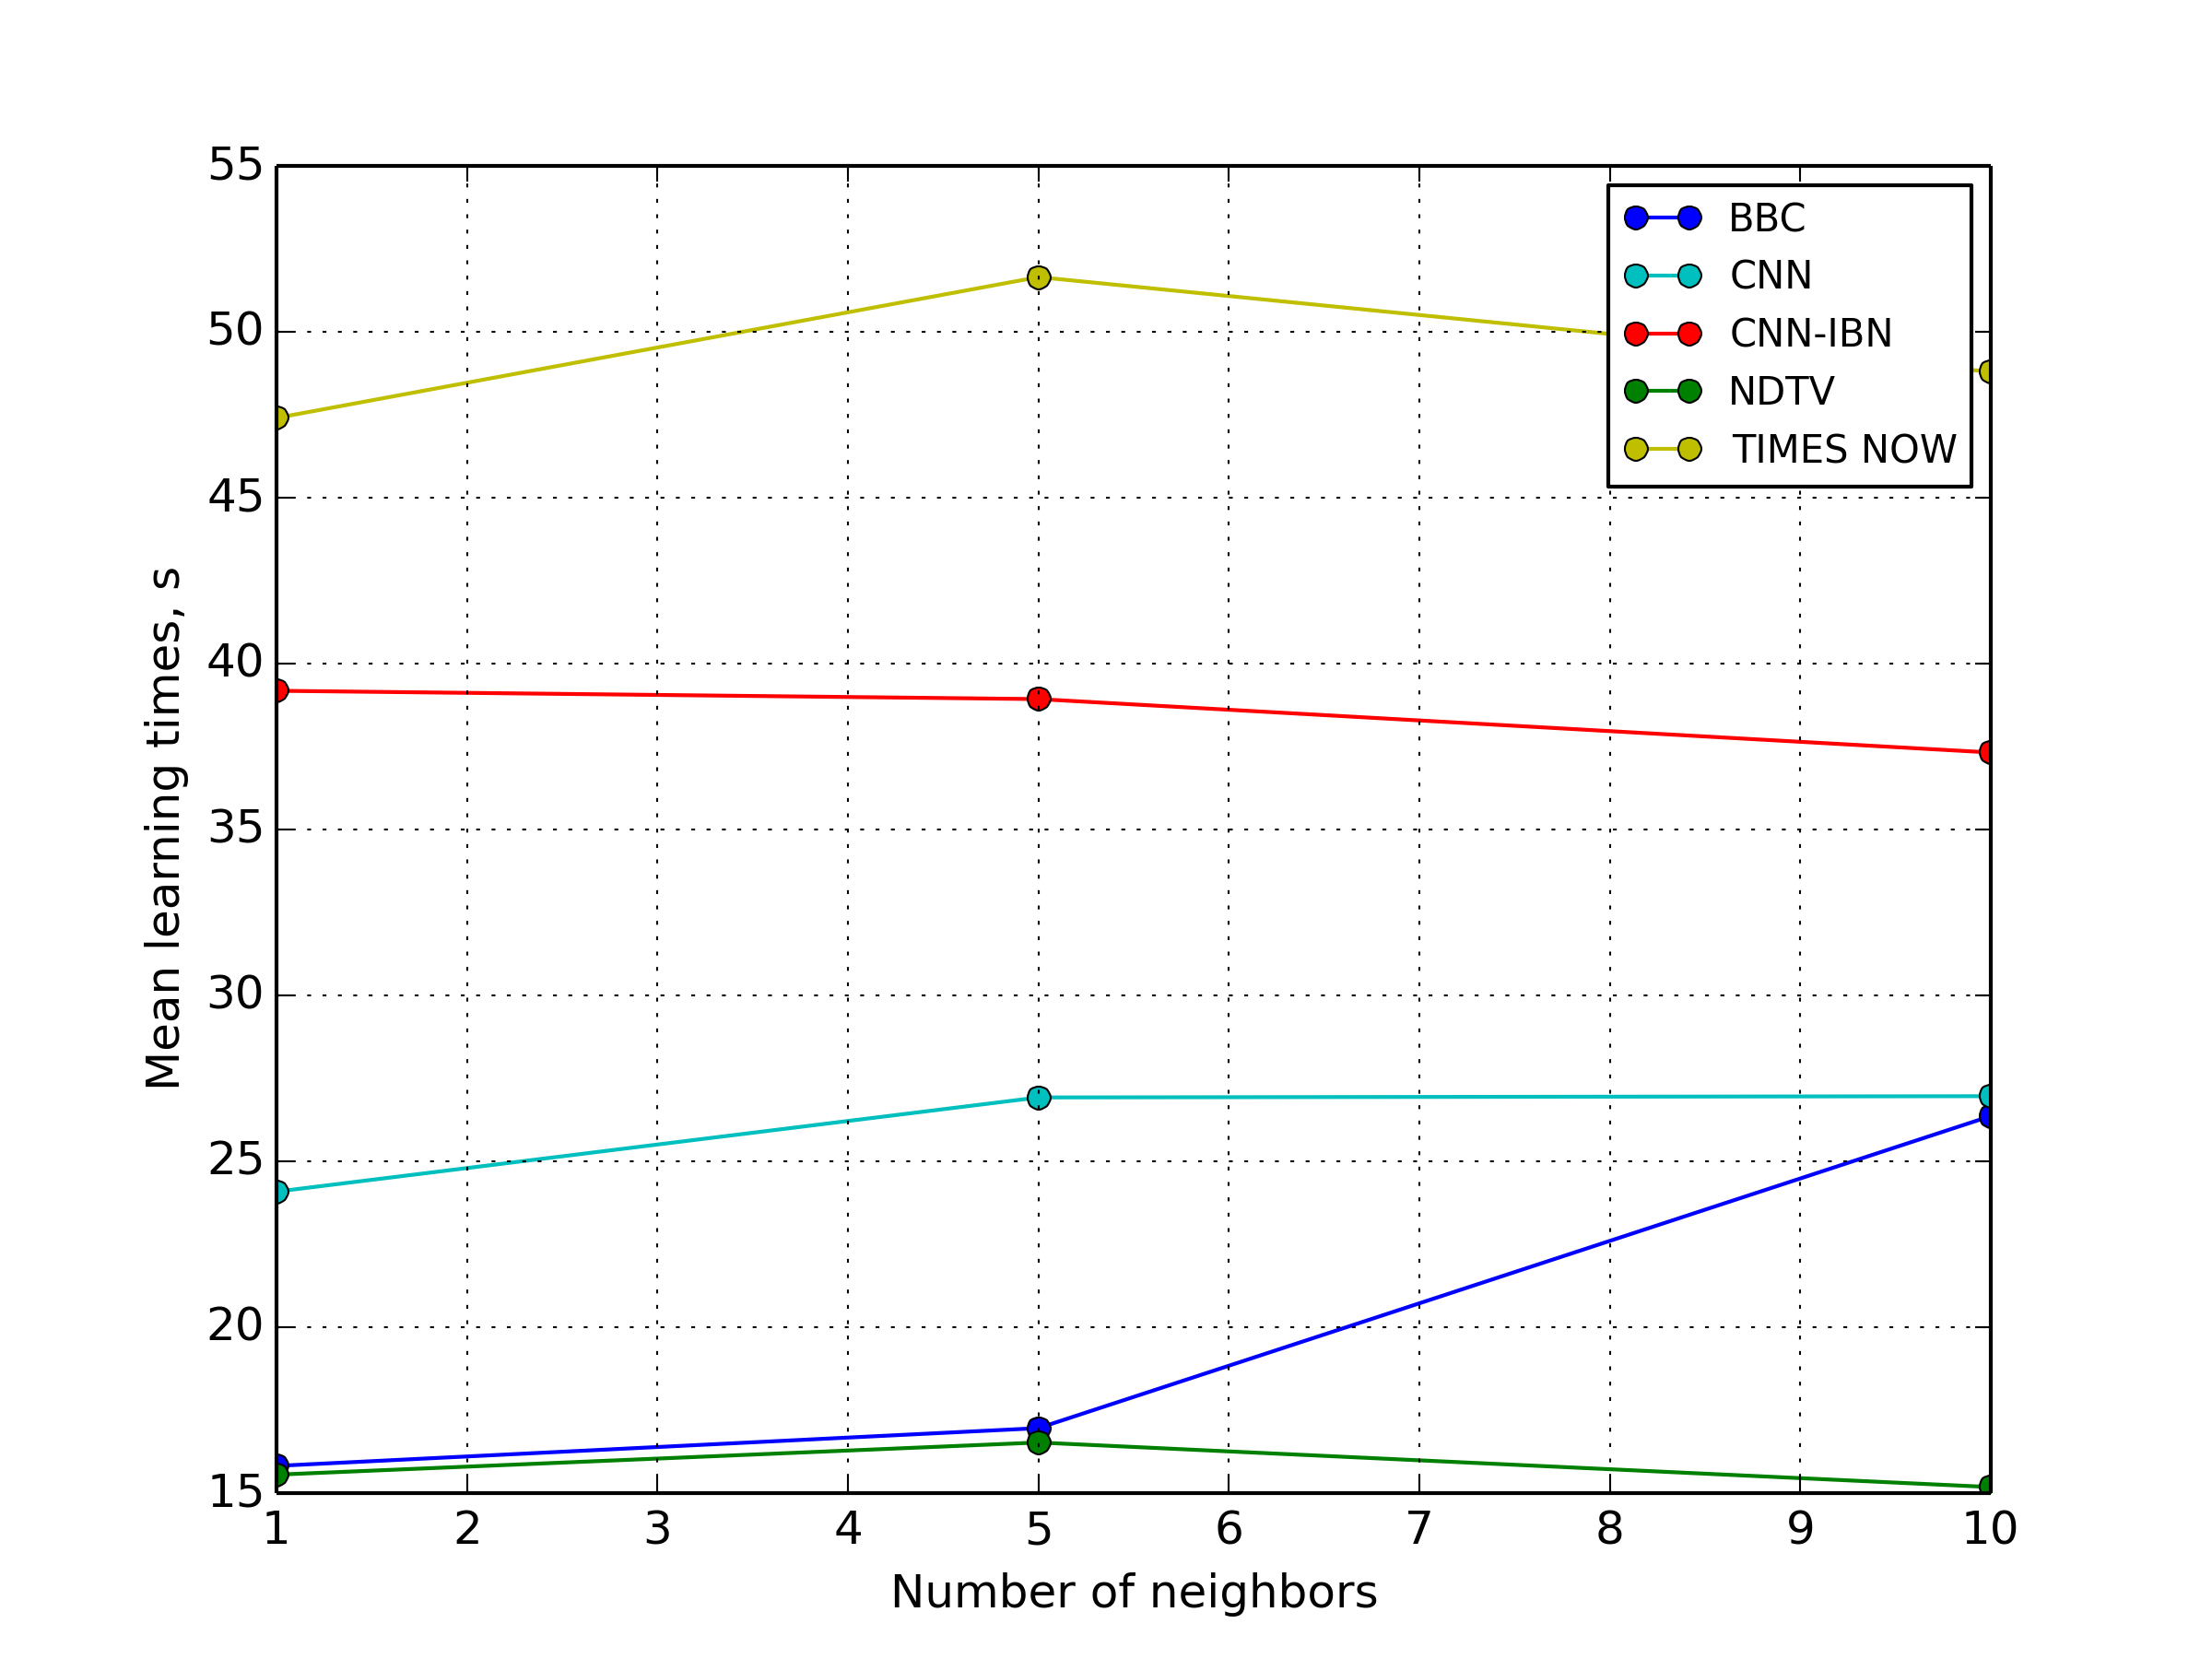
\includegraphics[width=\textwidth]{images/fcnn-gradboostingTime.png}
		\caption{Время обучения.}
	\end{subfigure}
	\caption{Результаты применения FCNN для GTB}\label{fig:fcnn-gtb-results}
\end{figure}

В таблице~\ref{table:fcnn-results} приведены результаты применения метода FCNN с правилом одного ближайшего соседа. Использованы обозначения, аналогичные таблице~\ref{table:cnn-results}.
\begin{table}[h!]
    \centering
    \begin{tabular}{|c||c||c|c|}
    \cline{2-4}
    \multicolumn{1}{c||}{} & Сжатие \(T\) & \(k\)NN & LDA \\
    \hline \hline
	\input{fcnn-table1.txt}
\end{tabular}
\newline \vspace*{0.5cm} \newline
\begin{tabular}{|c||c|c|c|}
    \cline{2-4}
    \multicolumn{1}{c||}{} & SVM & Random forest & GTB \\
    \hline \hline
	\input{fcnn-table2.txt}
    \end{tabular}
    \caption{Сводная таблица результатов метода FCNN и базовых методов после применения FCNN}
    \label{table:fcnn-results}
\end{table}

Во-первых, стоит отметить, что FCNN показал худшие, чем CNN, результаты по редукции обучающей выборки и времени работы (тем не менее, согласно \cite{angiulli}, FCNN имеет лучшую асимптотику по сравнению с CNN и, возможно, соотношение по времени работы было бы иным при редукции сверхбольшого набора данных). Во-вторых, FCNN показал хорошие результаты по сохранению обобщающей способности классификатора: качество классификации упало не более, чем на 1.8\% для всех методов и каналов. По этому параметру FCNN обогнал CNN. В-третьих, FCNN также позволил значительно сократить время работы метода 13 ближайших соседей и случайного леса. LDA, как и в случае с CNN требовал значительно больше (в относительных числах, абсолютное время обучения у LDA оставалось очень малым) времени на обучение модели.

\subsection{Class conditional instance selection}
CCIS \cite{marchiori} отличается от двух предыдущих методов тем, что он принадлежит к категории гибридных методов отбора эталонов. Он состоит из двух этапов: классово-условный выбор эталонов (CC) и прорежение (THIN).

Центральным для данного метода является граф классово-условных ближайших соседей \(G=(V,E)\) --- орграф, вершинам \(v\in V\) которого соответствуют элементы \(T\), а ребро \((a,b)\in E\), если \(b\) есть ближайший сосед \(a\) для некоторого класса. \(G\) разбивается на 2 подграфа: \(G_{wc}=(V,E_{wc})\), в котором есть лишь те рёбра из \(G\), которые инцидентны двум вершинам одного класса и \(G_{bc}=(V,E_{bc})\), в котором есть лишь те рёбра из \(G\), которые инцидентны двум вершинам разных классов. Полустепень захода в первом называется внутриклассовой полустепенью захода (within class in-degree), во втором --- междуклассовой полустепенью захода (between class in-degree).

Классово-условный отбор эталонов составляет подмножество \(S\) обучающей выборки \(T\), добавляя в него элементы по одному пока Leave-one-out-ошибка, полученная методом ближайшего соседа на \(S\), убывает и больше LOO-ошибки, полученной на \(T\). Порядок, в котором элементы \(T\) выбираются для добавления в \(S\), обусловлен теоретико-информационным критерием, зависящим от полустепеней захода элемента в \(G_{wc}\) и \(G_{bc}\), и характеризующим то, насколько глубоко объект находится внутри своего класса. В частности, из \(T\) удалятся все объекты, для которых междуклассовая полустепень захода больше внутриклассовой (такие элементы, скорее всего, лежат близко к границе классов.

Прорежение призвано отфильтровать \(S\), оставив объекты, наиболее важные для определения границы классов. Для этого из \(S\) выбирается подмножество \(S_f\), состоящее из объектов с положительной междуклассовой полустепенью захода в графе \(G^S\) для выборки \(S\) (эти объекты считаются важными для определения границы между классами). Затем \(S_f\) дополняется объектами из \(S\setminus S_f\) пока LOO-ошибка на \(T\) при использовании \(S\) в качестве обучающей выборки уменьшается.


\section{Заключение}
В работе был дан обзор базовых методов машинного обучения и исследована их эффективность применительно к модельной задаче по распознаванию рекламы. На первом этапе произведен подбор основных параметров методов с целью получения оптимального качества классификации на исходных данных. Как и ожидалось, простые методы (
\(k\)NN, LDA) показали не лучшее классификации, но зато они быстро работают. Более продвинутые методы работают медленнее и для них имеет смысл использовать селекцию признаков или эталонов (см. таблицу \ref{table:base-all}). 
\par

\printbibliography
\end{document}

